\section{Reduction  to band bidiagonal form}
\label{sec:band}
The idea of using a tile algorithm to factorize a full matrix into
a band bidiagonal one is not new.
The approach was first introduced in 2010 by
Dongarra~et~al\@.~\cite{ltaief2010parallel},
and improved in 2013~\cite{haidar2013improved}
by the same authors.
This section aims at evaluating different options for
designing such an algorithm
before moving to the second stage of the factorization.

We identified two main design options:
(1) a ``late update'' strategy, and
(2) an ``early update'' strategy.
Each of these strategies are introduced
and assessed in the subsections below.

\subsection{Late update strategy}
To reduce a full $mt \times nt$ tile matrix $A$ to a band bidiagonal
form, the late update strategy begins by applying a QR
factorization to the first panel $A(1:mt,1)$ (using MATLAB indexing)
(see Figure~\ref{fig:qr_1}), then updating the trailing
submatrix $A(1:mt,2:nt)$ (Figure~\ref{fig:qr_update_1}), followed
by an LQ factorization of the first tile-row,
ignoring the first column (Figure~\ref{fig:lq_1}),
and the update of the corresponding trailing matrix
(Figure~\ref{fig:lq_update_1}).
This procedure is repeated until the whole matrix is reduced to
band bidiagonal form, as illustrated in Figure~\ref{fig:panel}.
It is important to notice that we describe this strategy
at tile-column (panel) and tile-row granularity but
tile algorithms are used underneath to process each panel
and the update of the trailing matrix.
We can think of this as a direct translation of the LAPACK
column-oriented procedure into a
more modern tile-based algorithm.

\begin{figure}[h!]
  %%%% 1
  \captionsetup[subfigure]{justification=justified,singlelinecheck=false}

  \begin{subfigure}[t]{0.2 \textwidth}
    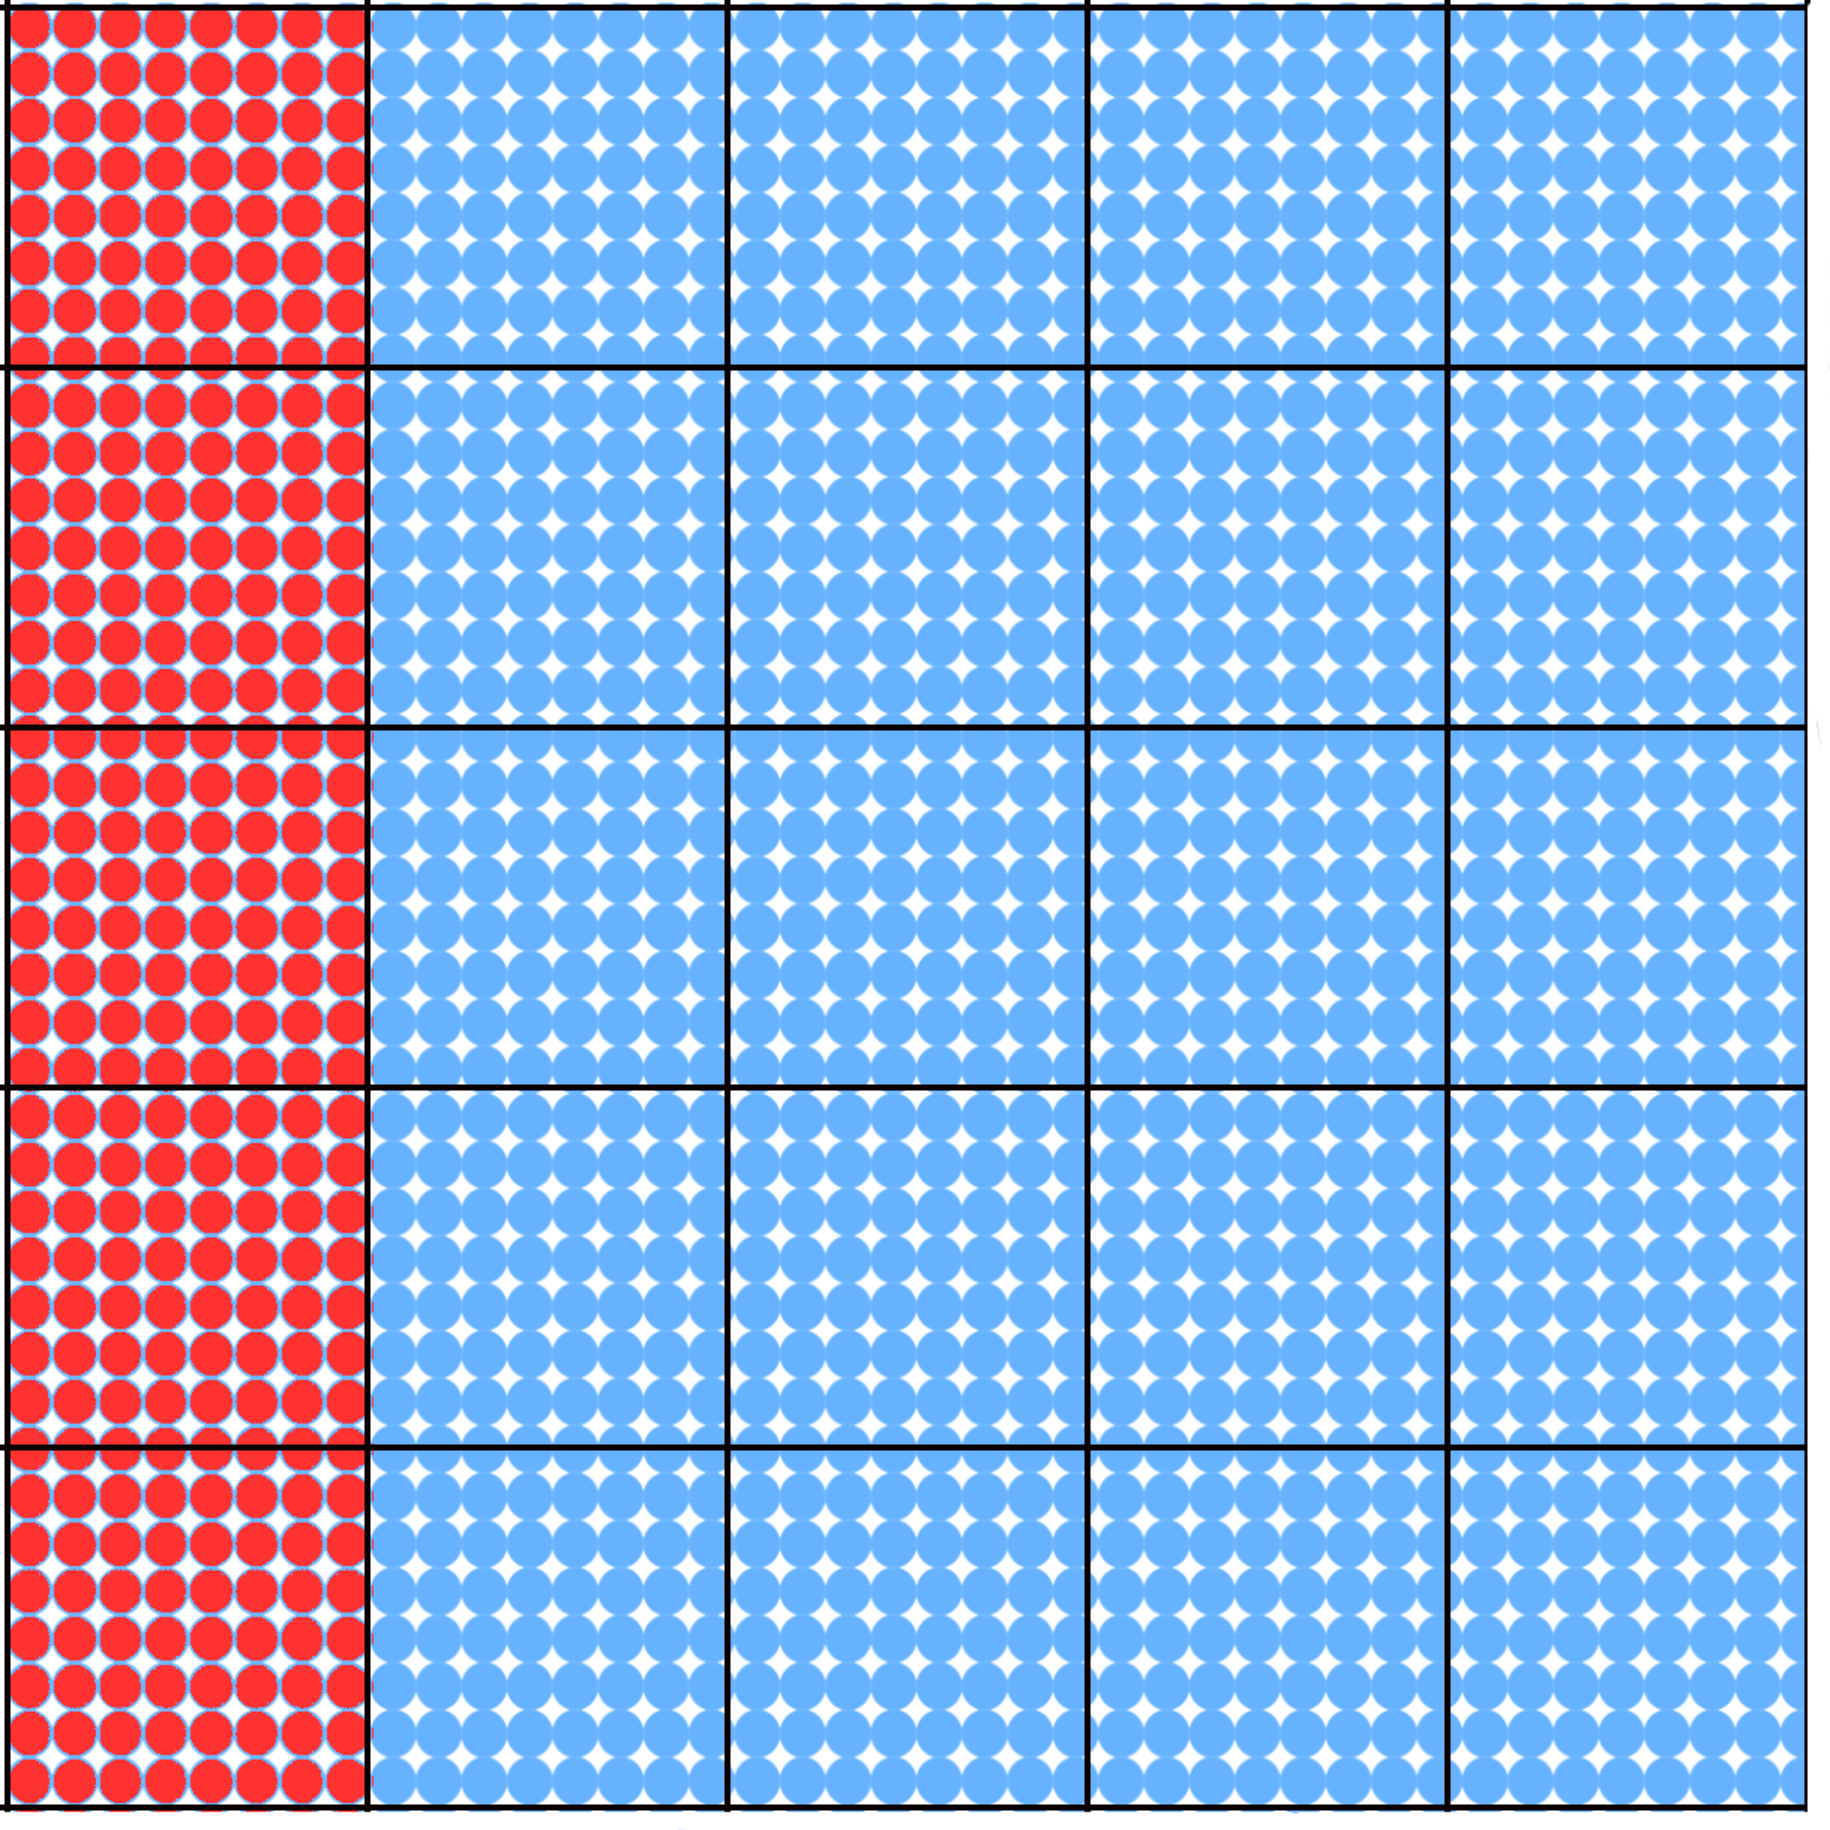
\includegraphics[width=\textwidth]{fig/SVD_panel_1_grid}
    \caption{\label{fig:qr_1}\small{Panel QR}}
  \end{subfigure}
  \hfill
  %%%% 2
  \begin{subfigure}[t]{0.2 \textwidth}
    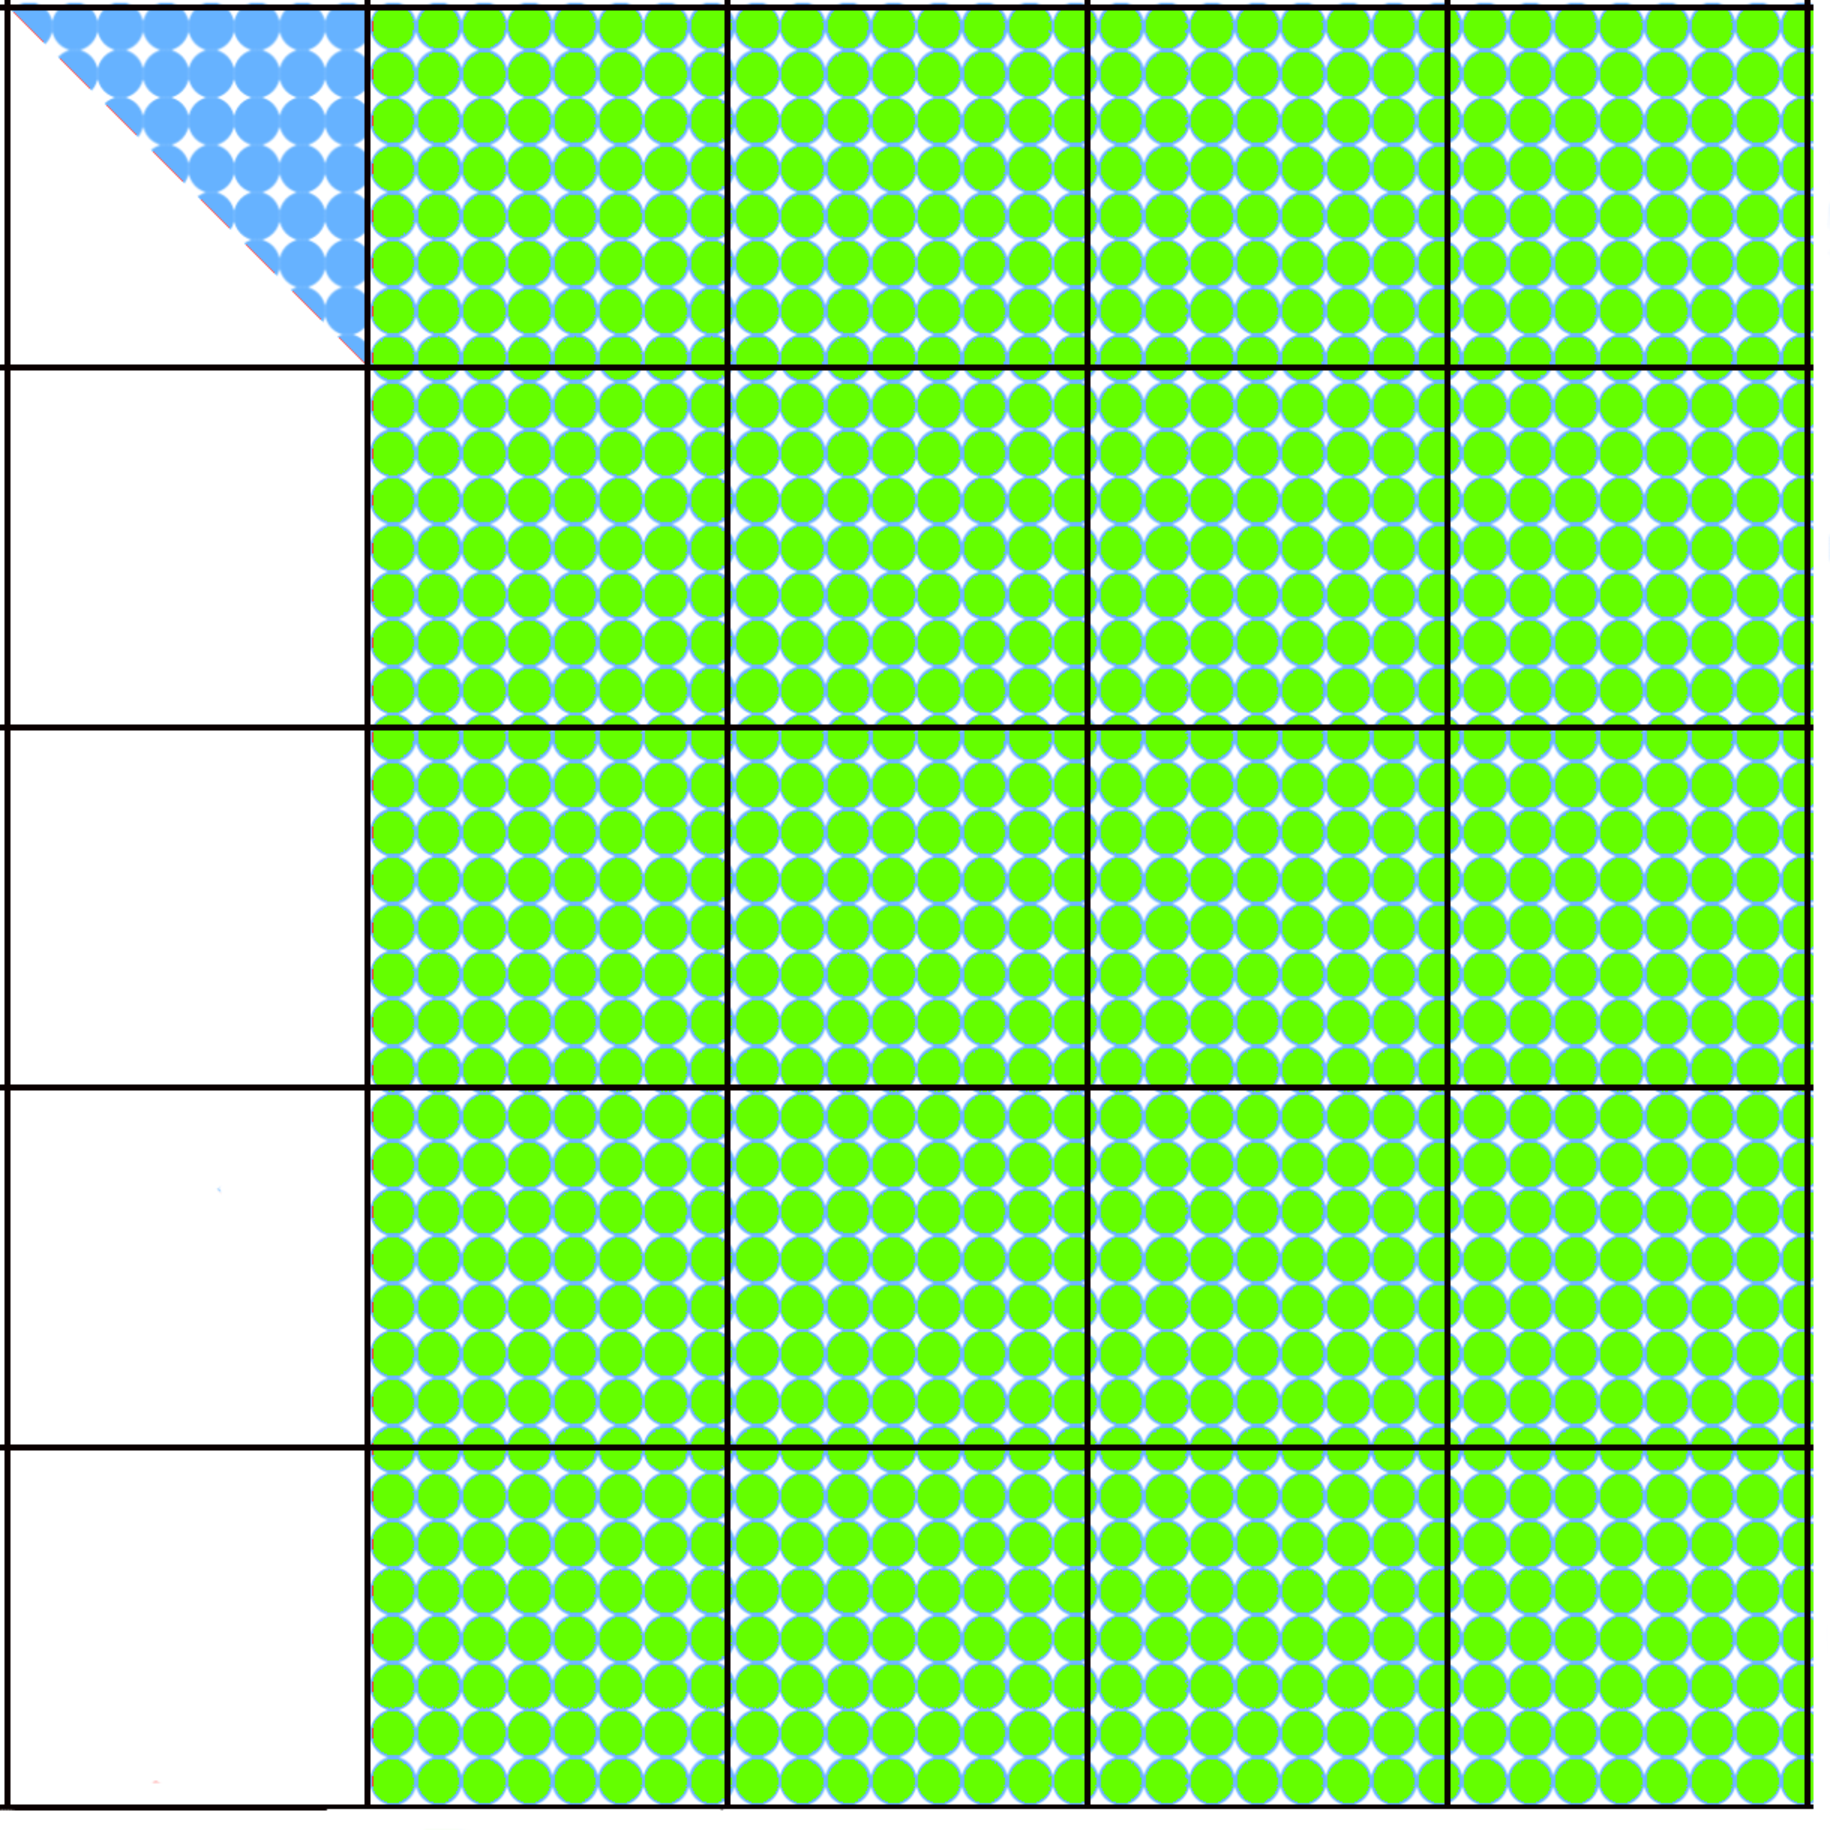
\includegraphics[width=\textwidth]{fig/SVD_panel_2_grid}
    \caption{\label{fig:qr_update_1}Update}
  \end{subfigure}
  \hfill
  %%%% 3
    \begin{subfigure}[t]{0.2 \textwidth}
    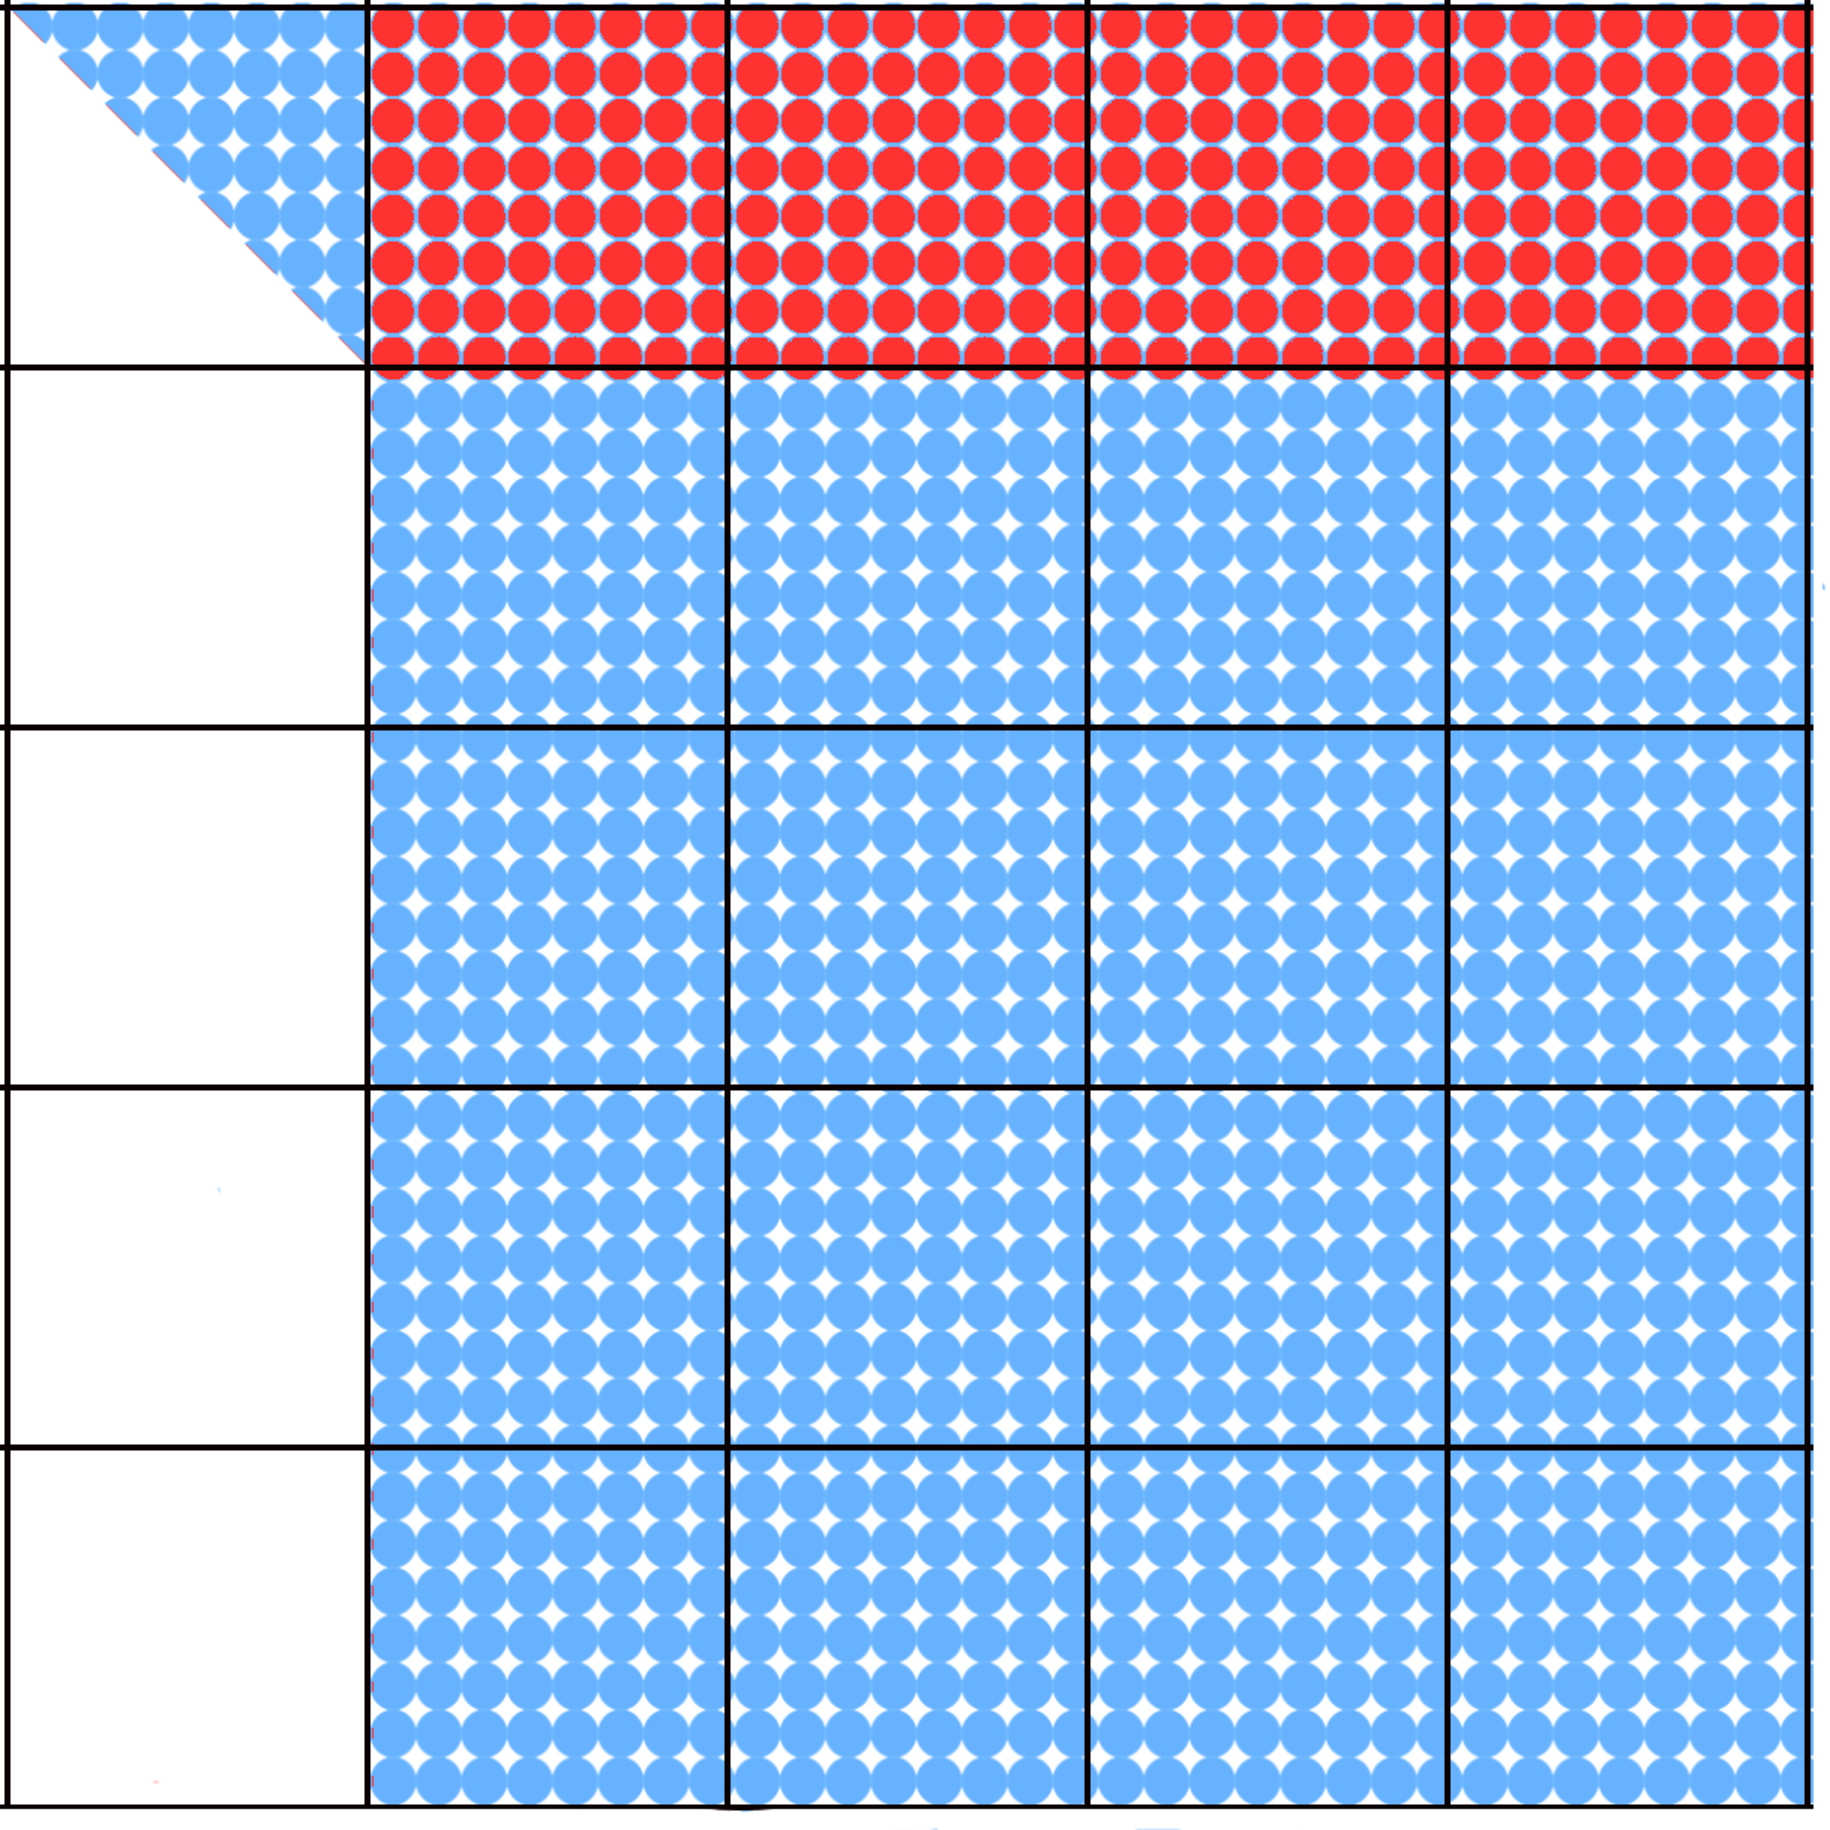
\includegraphics[width=\textwidth]{fig/SVD_panel_3_grid}
    \caption{\label{fig:lq_1}\small{Tile-row LQ}}
    \end{subfigure}
    \hfill
    %%%% 4
    \begin{subfigure}[t]{0.2 \textwidth}
      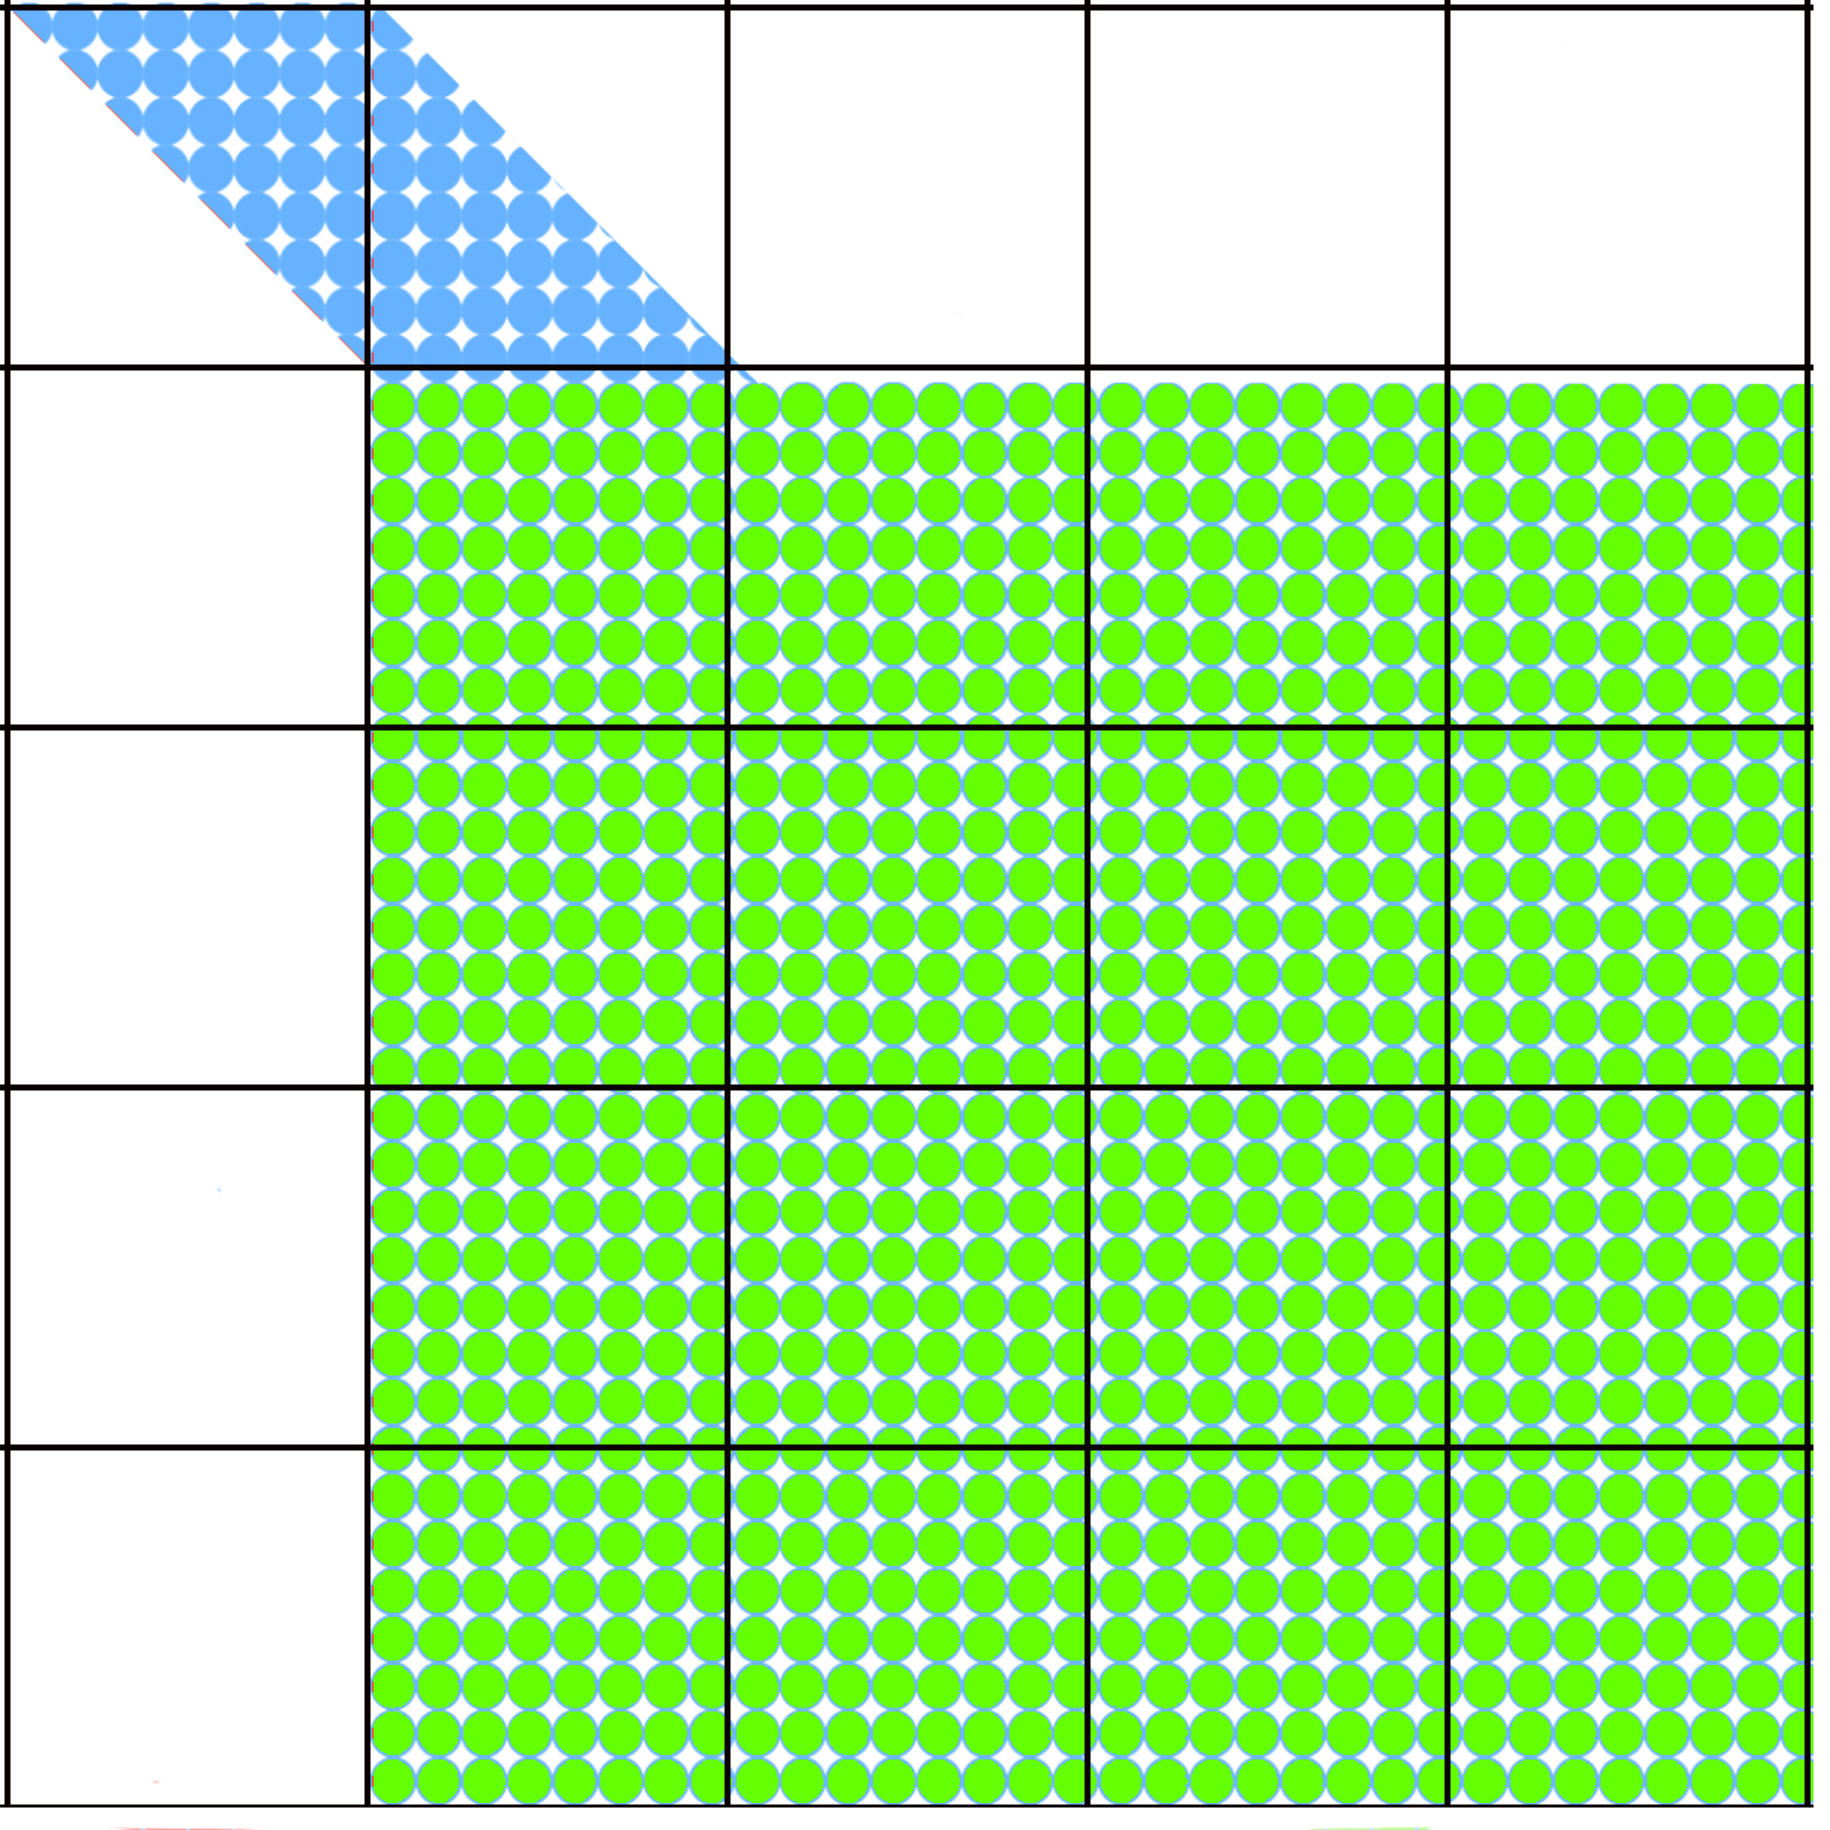
\includegraphics[width=\textwidth]{fig/SVD_panel_4_grid}
      \caption{\label{fig:lq_update_1}Update}
    \end{subfigure}
    \hfill
    %%%% 5
    \begin{subfigure}[t]{0.2 \textwidth}
      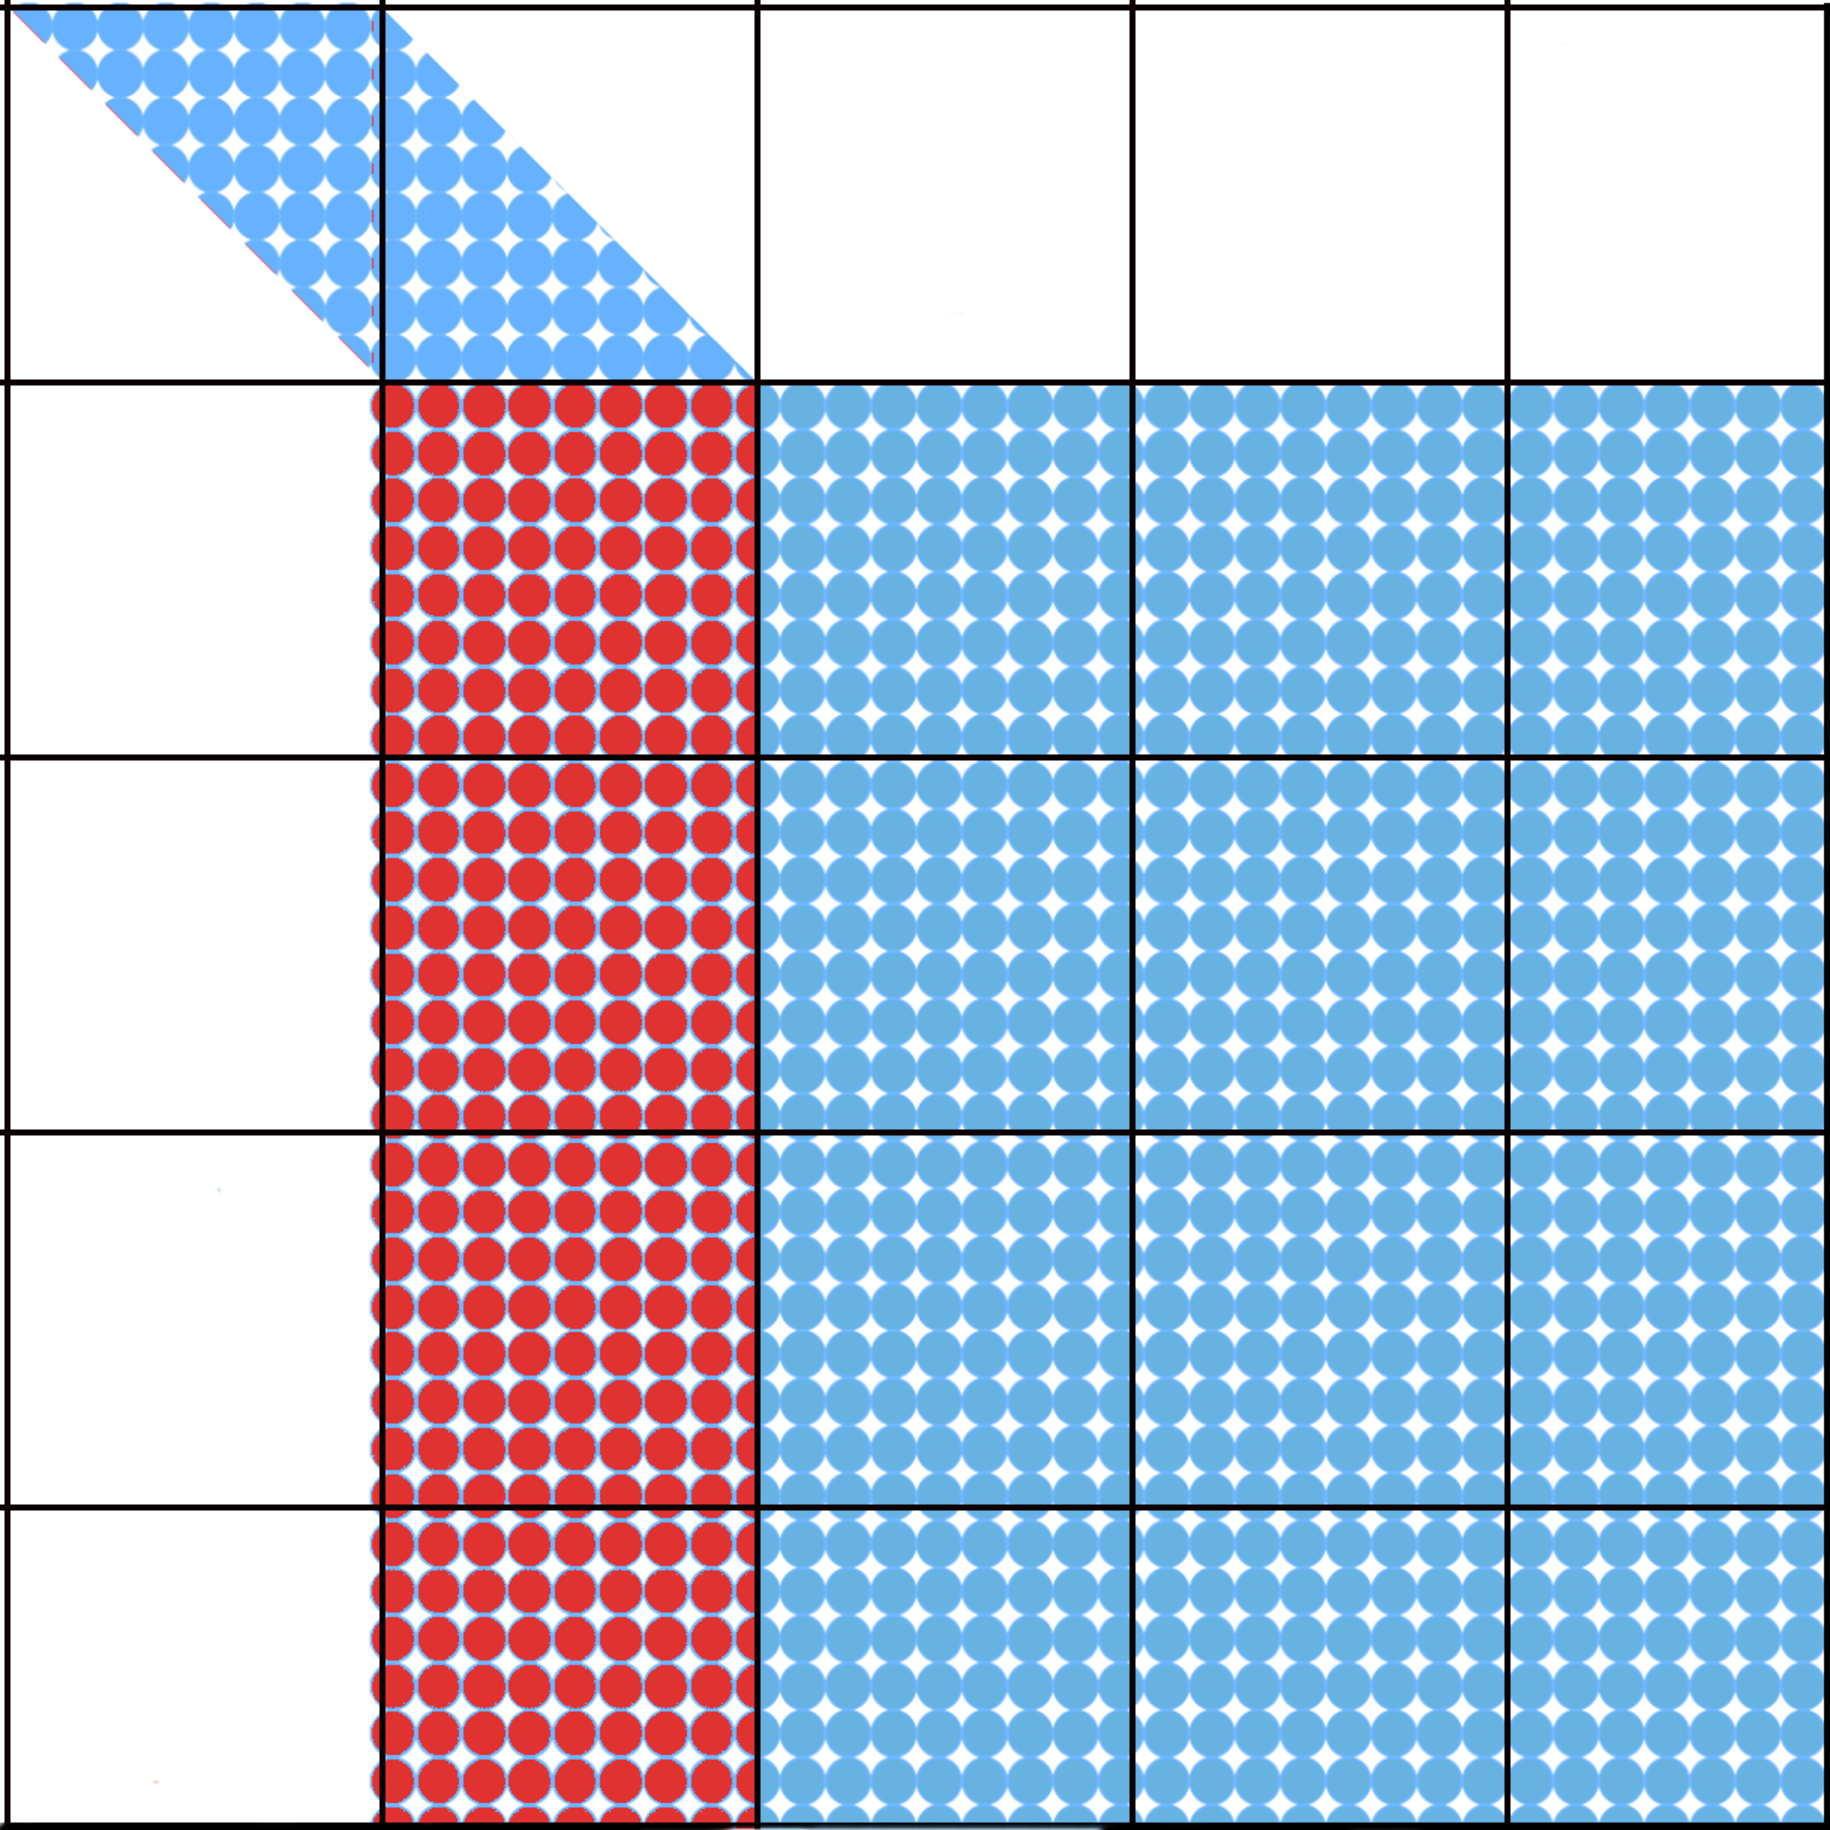
\includegraphics[width=\textwidth]{fig/SVD_panel_5_grid}
      \caption{\label{fig:qr_2}Panel QR}
    \end{subfigure}
    \hfill
    %%%% 6
    \begin{subfigure}[t]{0.2 \textwidth}
      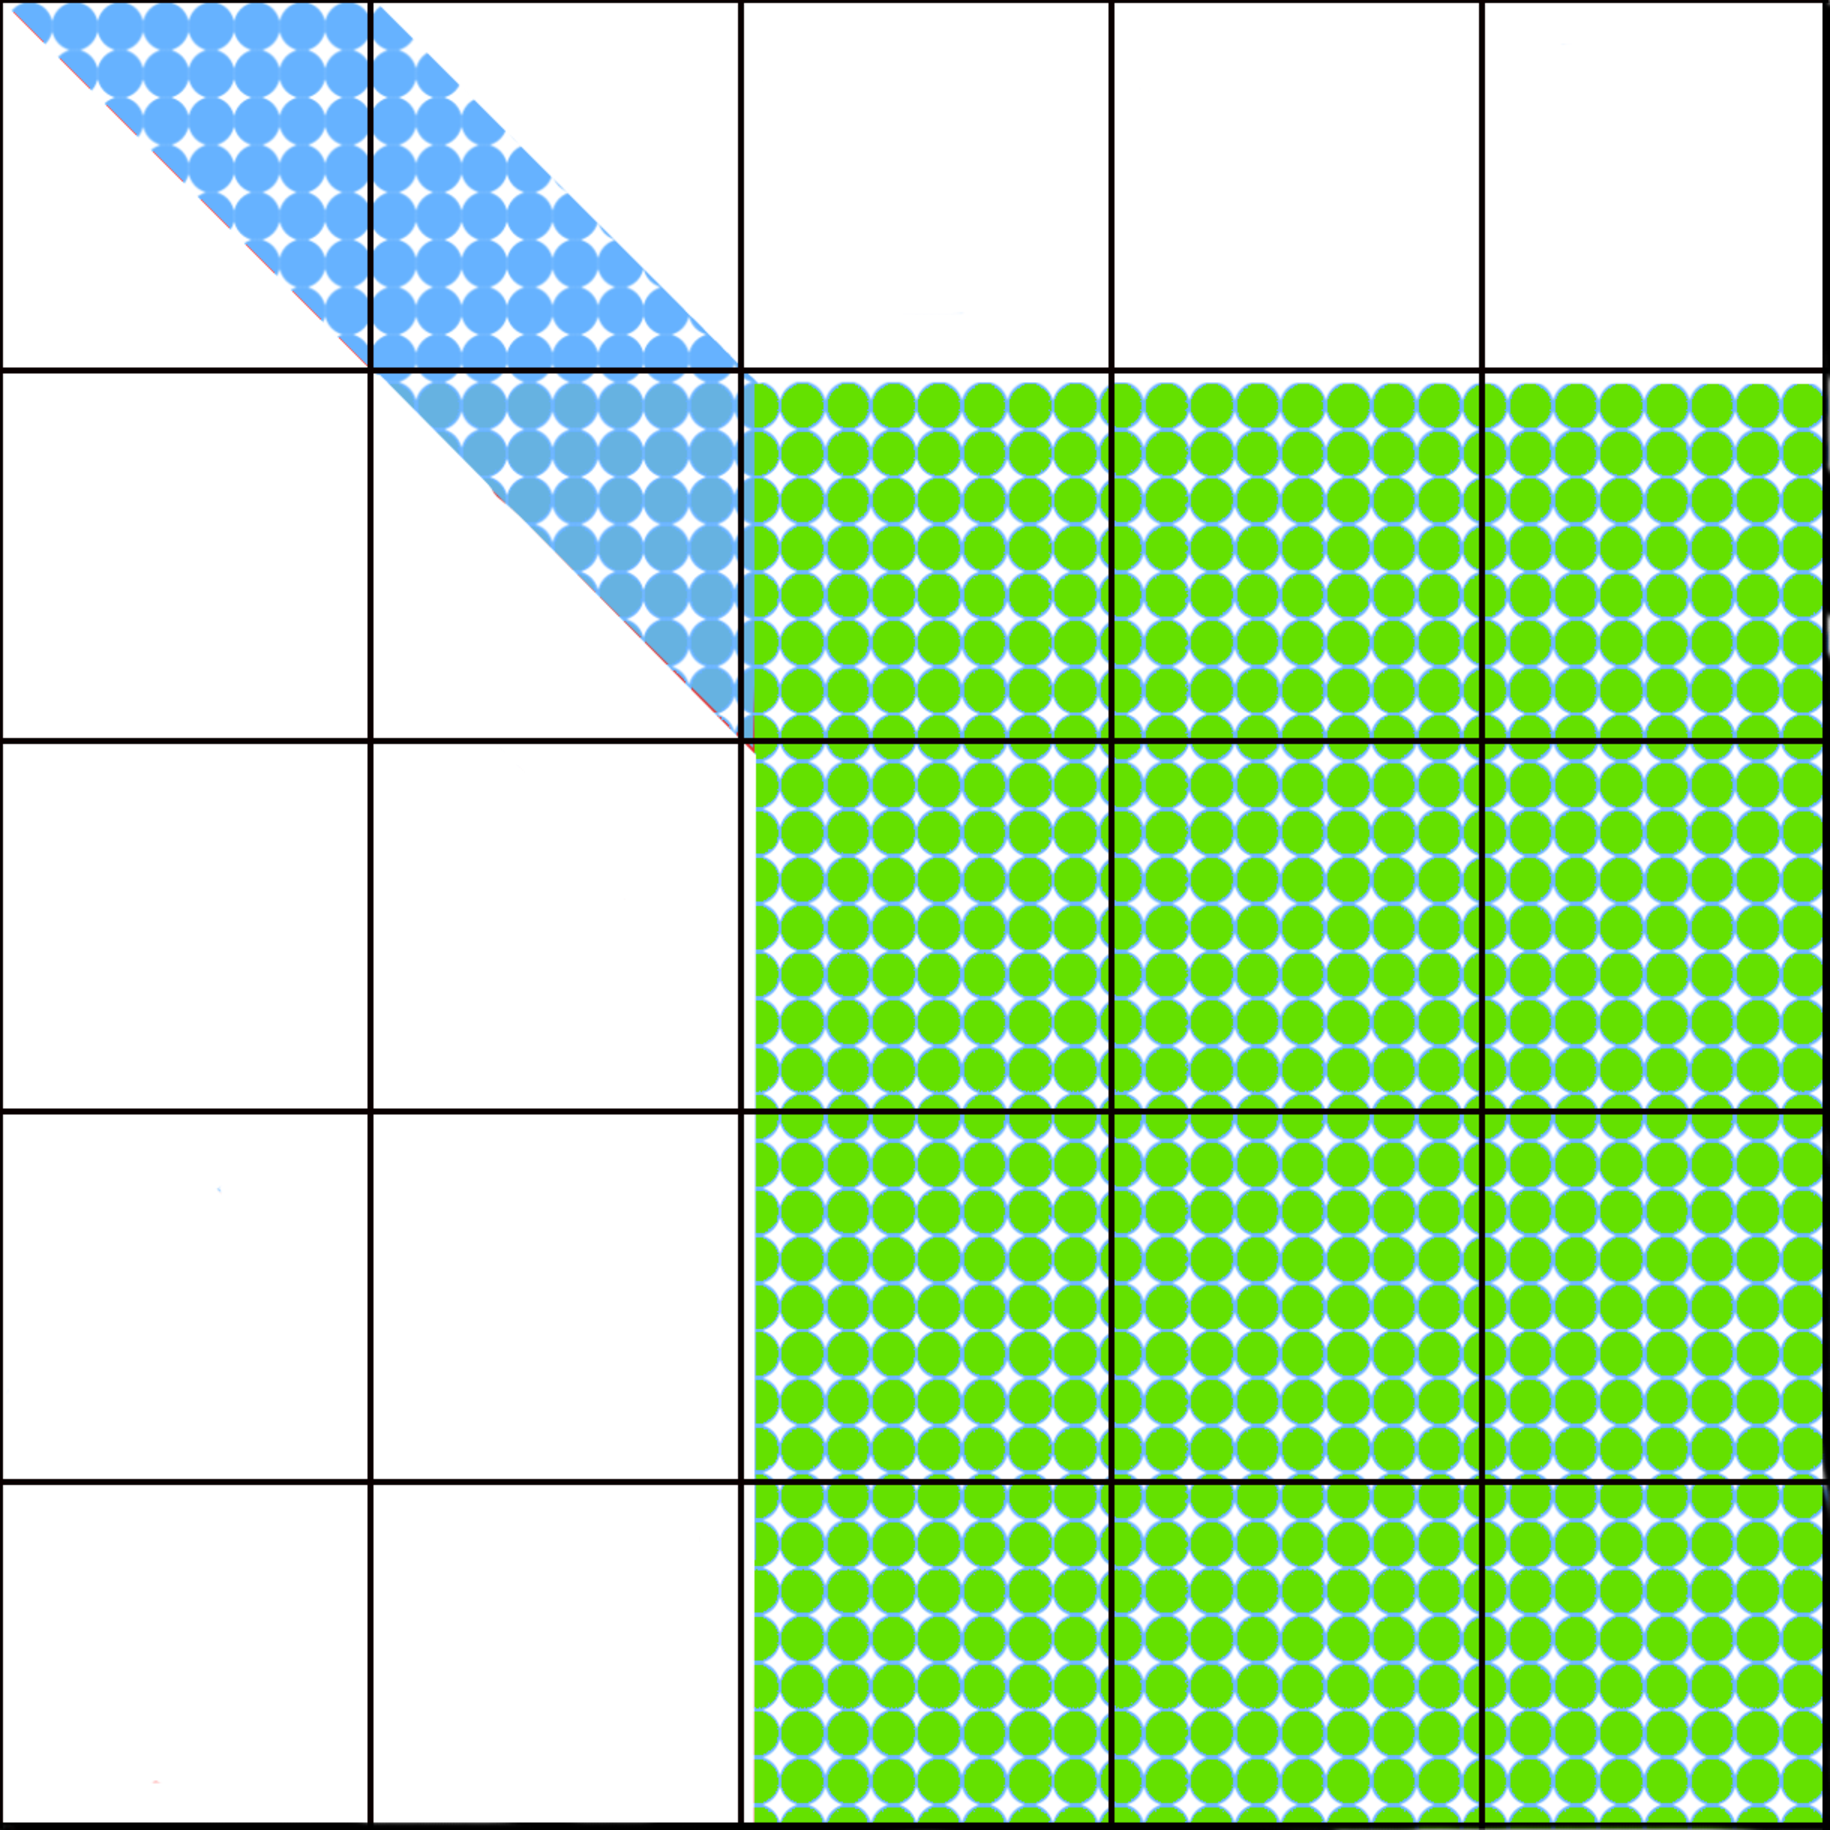
\includegraphics[width=\textwidth]{fig/SVD_panel_6_grid}
      \caption{\label{fig:qr_update_2}Update}
    \end{subfigure}
    \hfill
    %%%% 7
    \begin{subfigure}[t]{0.2 \textwidth}
      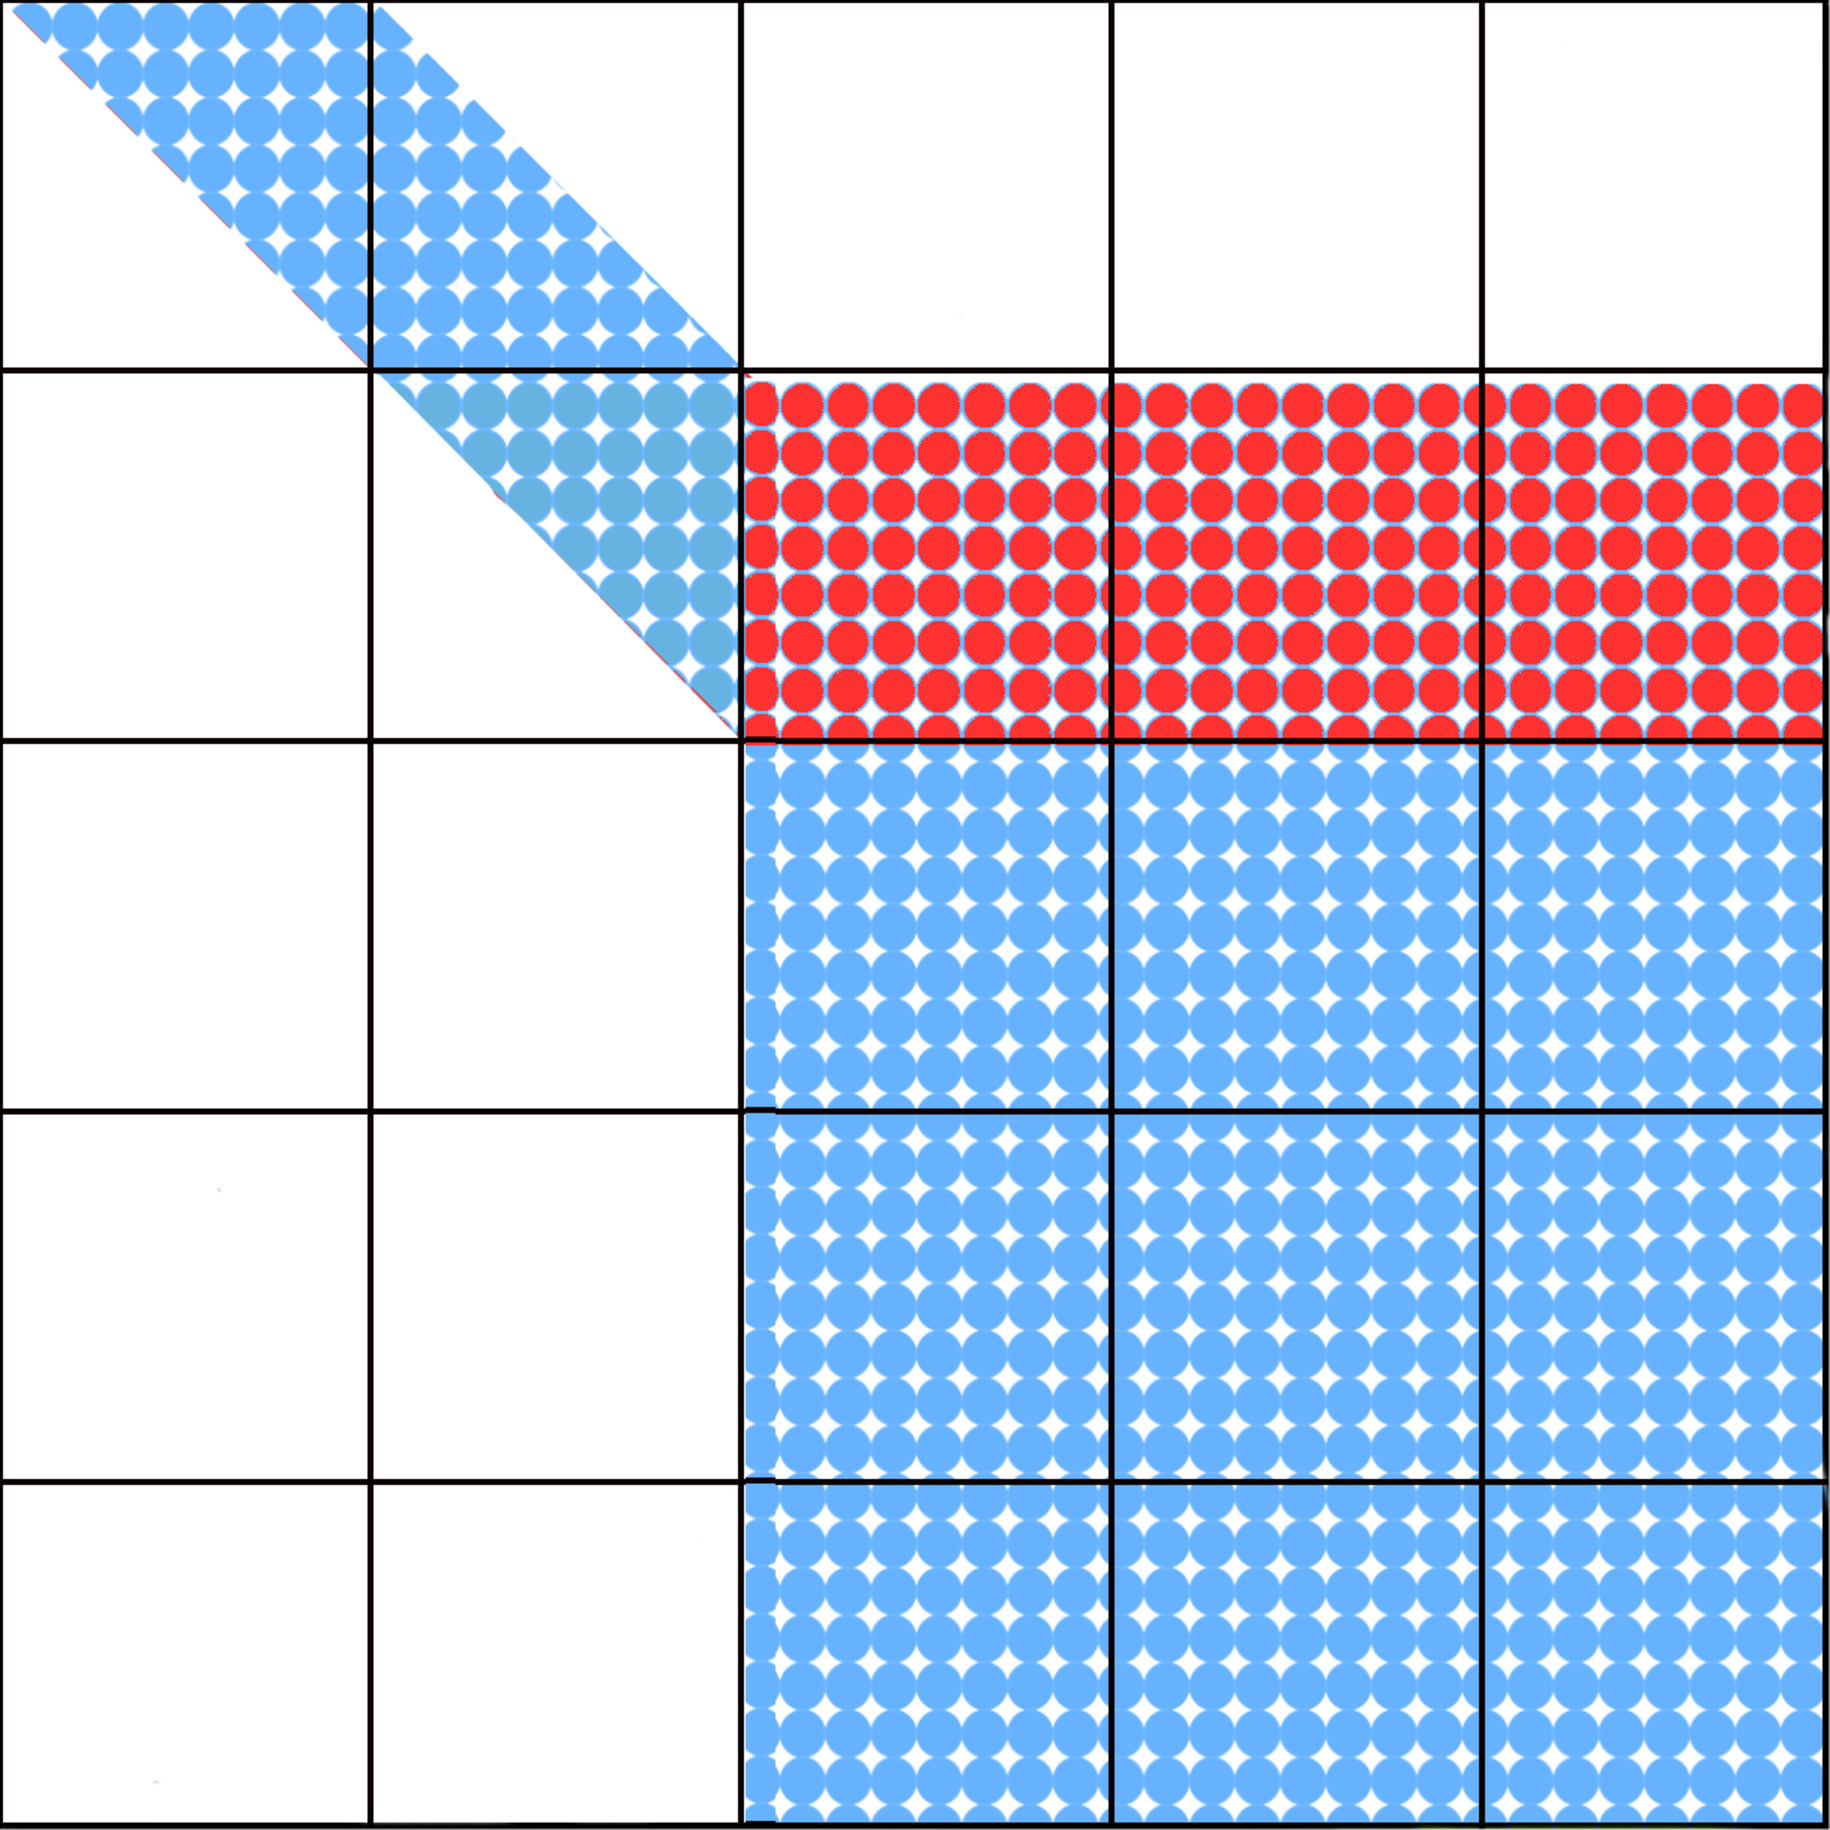
\includegraphics[width=\textwidth]{fig/SVD_panel_7_grid}
      \caption{\label{fig:lq_2}Row-tile LQ}
    \end{subfigure}
    \hfill
    %%%% 8
    \begin{subfigure}[t]{0.2 \textwidth}
      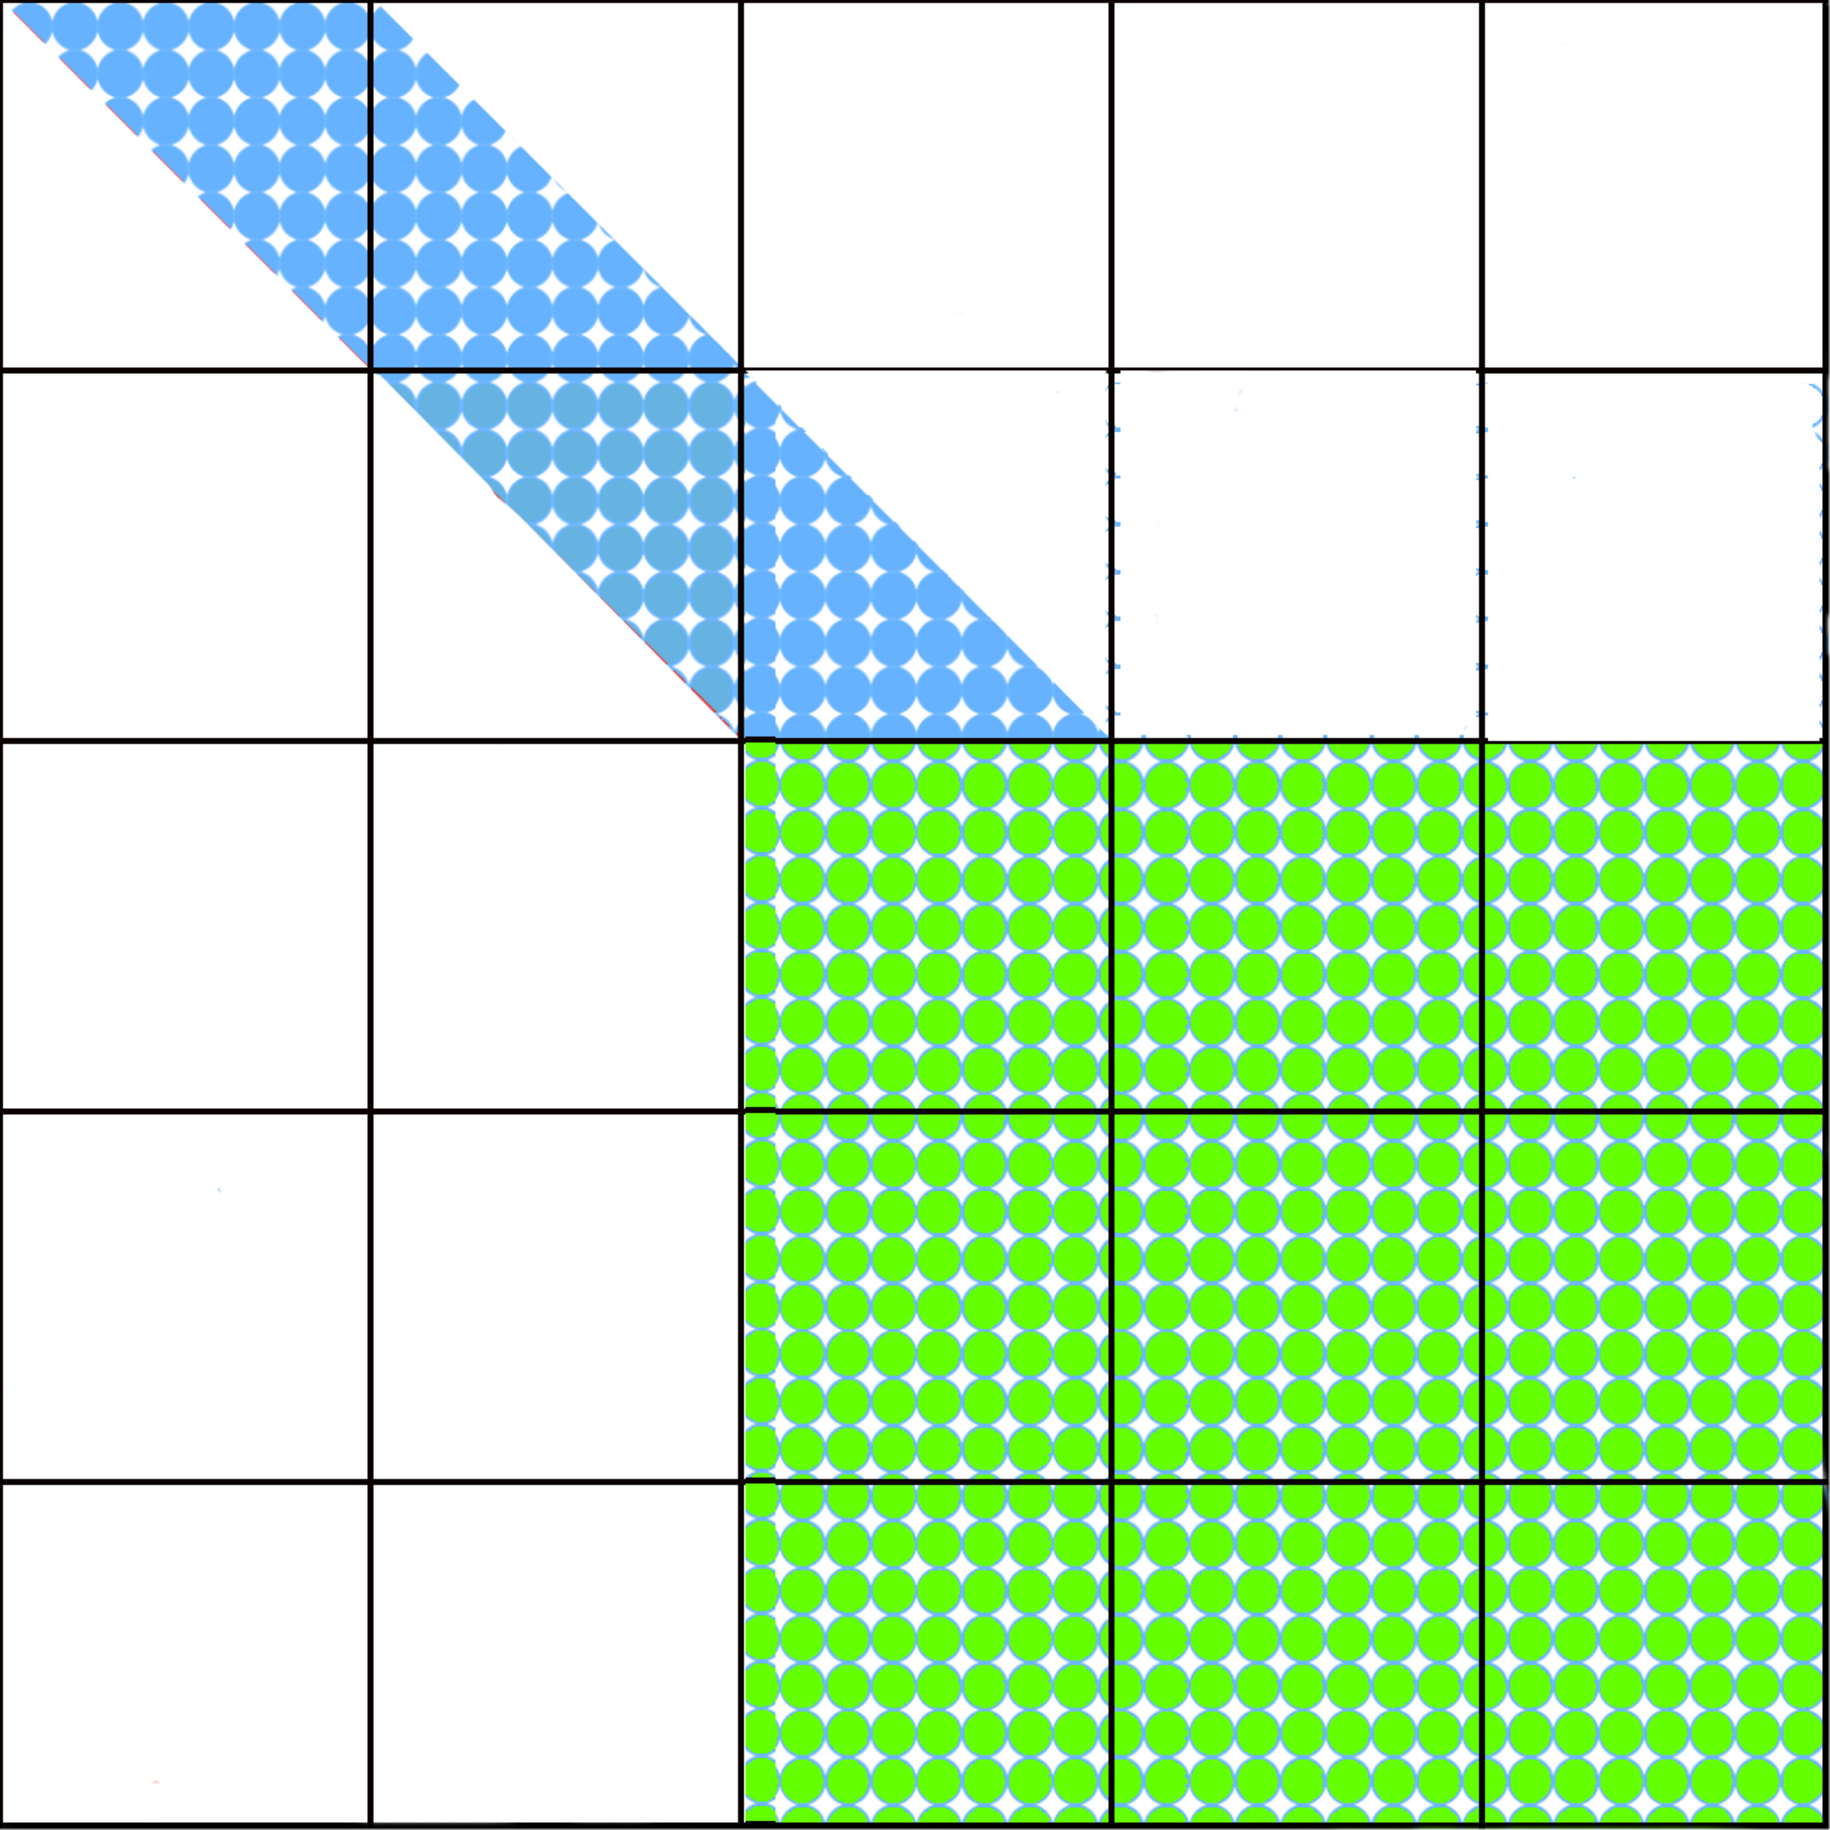
\includegraphics[width=\textwidth]{fig/SVD_panel_8_grid}
      \caption{\label{fig:lq_update_2}Update}
    \end{subfigure}
    \caption{Reduction from general matrix to band bidiagonal form
      using the late update strategy.
    \label{fig:panel}}
\end{figure}

The main advantage of this strategy is its simplicity,
the algorithm is very close to the LAPACK version. However the
individual steps of the QR factorization illustrated in
Figure~\ref{fig:rect_panel},
shows that a full factorization of a panel
starts with the $QR$ factorization of the first tile
(Figure~\ref{fig:geqrt_1}), which means only one CPU core is busy
while the others remain idle. Once the first tile is factorized, the
rest of work (to annihilate the tiles below using the TSQRT
kernel) can commence.
Since the elimination procedure modifies the entries of the
top triangular tile, only one square tile can be eliminated at a time
to guarantee a correct result.
Put differently,
the panel factorization introduces synchronization points
in the algorithm that
may lead to performance penalties.
The sequential nature of the panel factorization can be
clearly observed in Figure~\ref{fig:dag_panel},
which shows the DAG of the corresponding operations.

\begin{figure}
  \begin{center}
    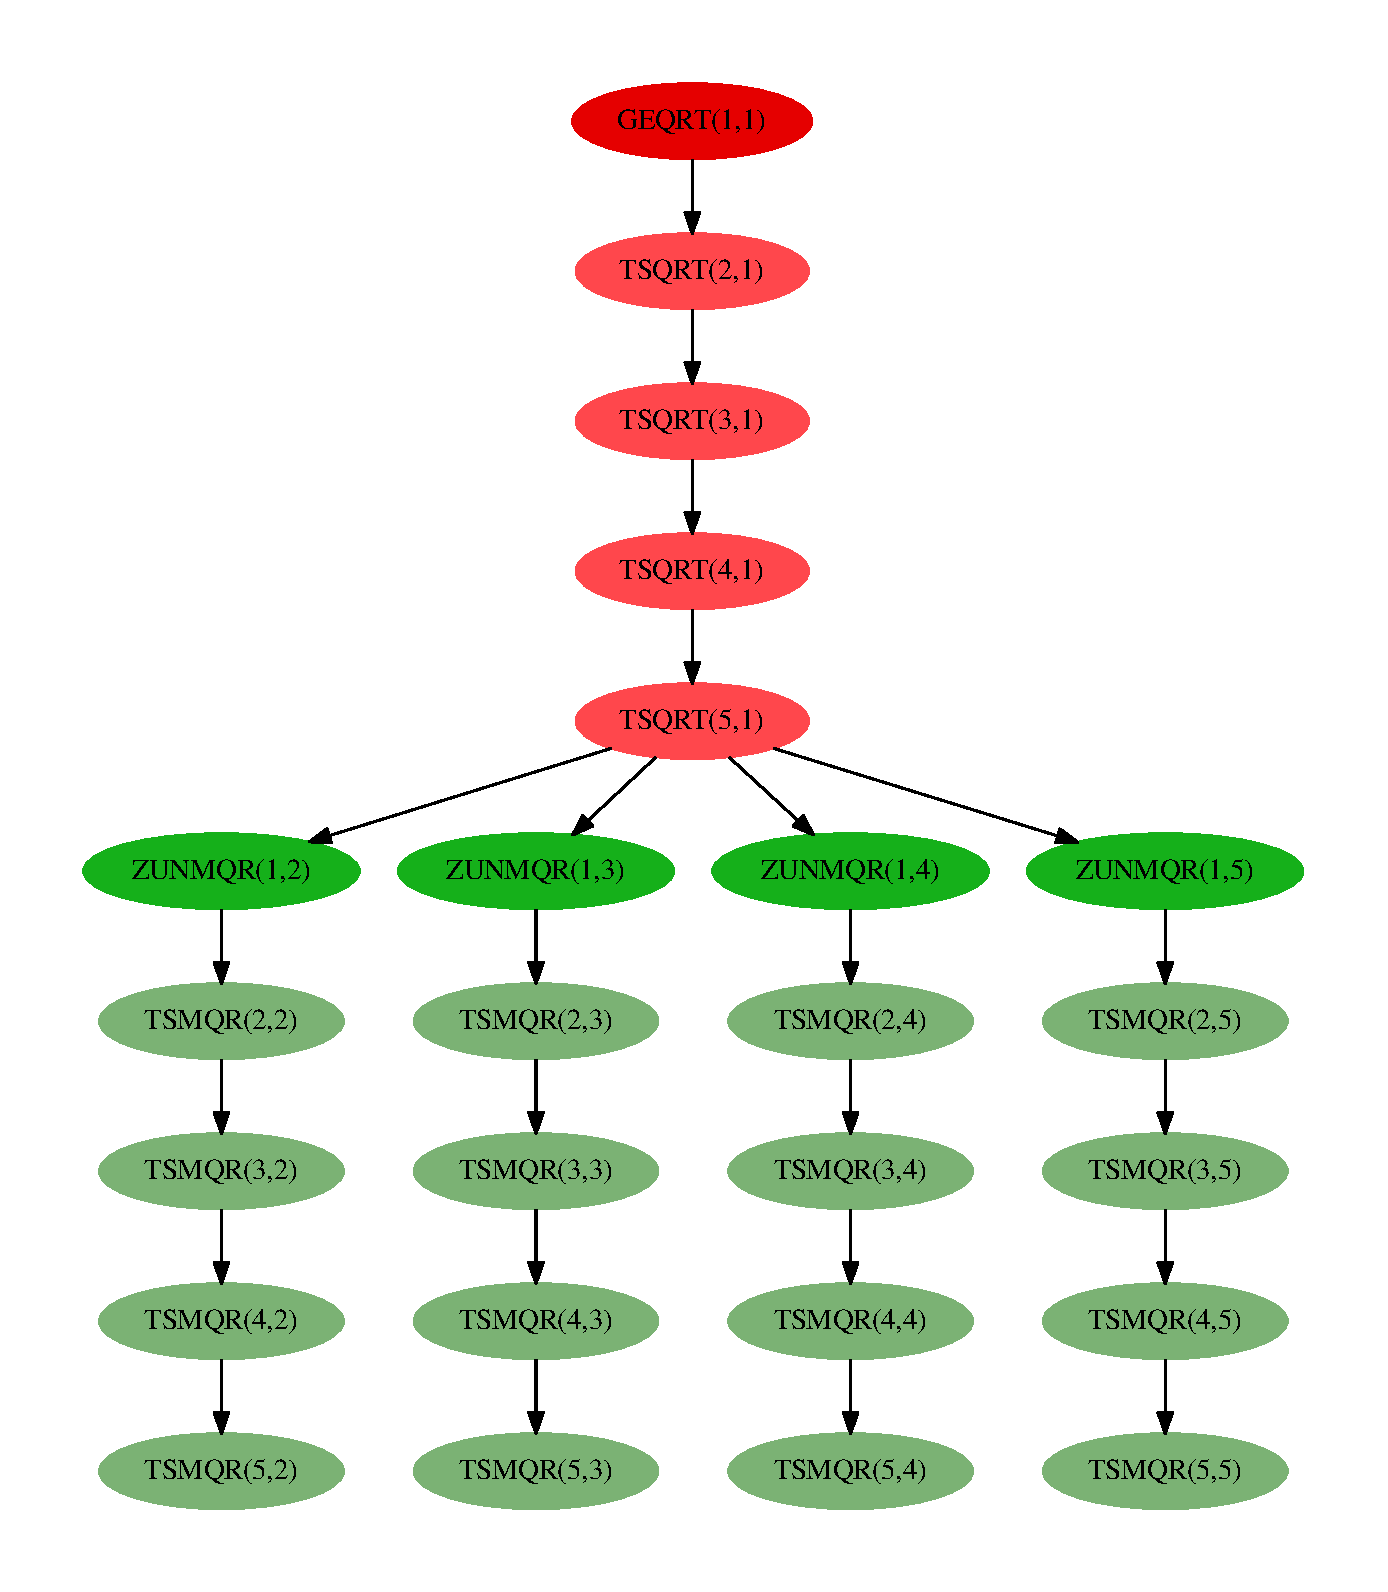
\includegraphics[width=0.5\textwidth]{fig/dag}
  \end{center}
  \caption{DAG of the late update strategy for band reduction:
    this partial view is limited to the factorization of the first panel and
    the update of the corresponding trailing matrix.}
  \label{fig:dag_panel}
\end{figure}

One can overcome this synchronization issue by overlapping the panel
factorization and the update steps.
As long as we respect the data dependencies, the algorithm can then progress onto the next step even
though the previous step is not completed.
In addition, when working on a panel we can
take advantage of ``tall and skinny'' QR factorization
strategies:
providing elegant methods to introduce parallelism
during a panel factorization.
This leads us to the early update strategy.

\subsection{Early update strategy}
To reduce a full tile matrix to a band bidiagonal form,
the early update strategy also completes the QR factorization
of the first panel and the update before starting the LQ process,
but the operations are launched in a completely different order.
Instead of completing the full factorization of a panel
before applying the updates as before,
the early update strategy looks down the panel,
factorizes each tile, and then launches
its corresponding updates immediately.

As depicted in Figure~\ref{fig:tile}, the algorithm starts with the
factorization of the tile $A(1,1)$ (Figure~\ref{fig:tile_qr_1}),
before applying the corresponding transformations to the rest of the
tile-row (Figure~\ref{fig:tile_qr_update_1}).
Once the first tile is factorized,
the remaining tiles in the panel are successively eliminated
and, in the same way, the trailing submatrices are updated immediately
(as illustrated in Figures~\ref{fig:tile_qr_2}
and~\ref{fig:tile_qr_update_2}
as well as in Figures~\ref{fig:tile_qr_3}
and~\ref{fig:tile_qr_update_3}).
In addition,
the updates in Figure~\ref{fig:tile_qr_update_2} can be computed in parallel
with the next tile elimination in Figure~\ref{fig:tile_qr_3}.
The same approach is used during the LQ factorization step.

\begin{figure}[h!]
  %%%% 1
  \begin{subfigure}{0.2 \textwidth}
    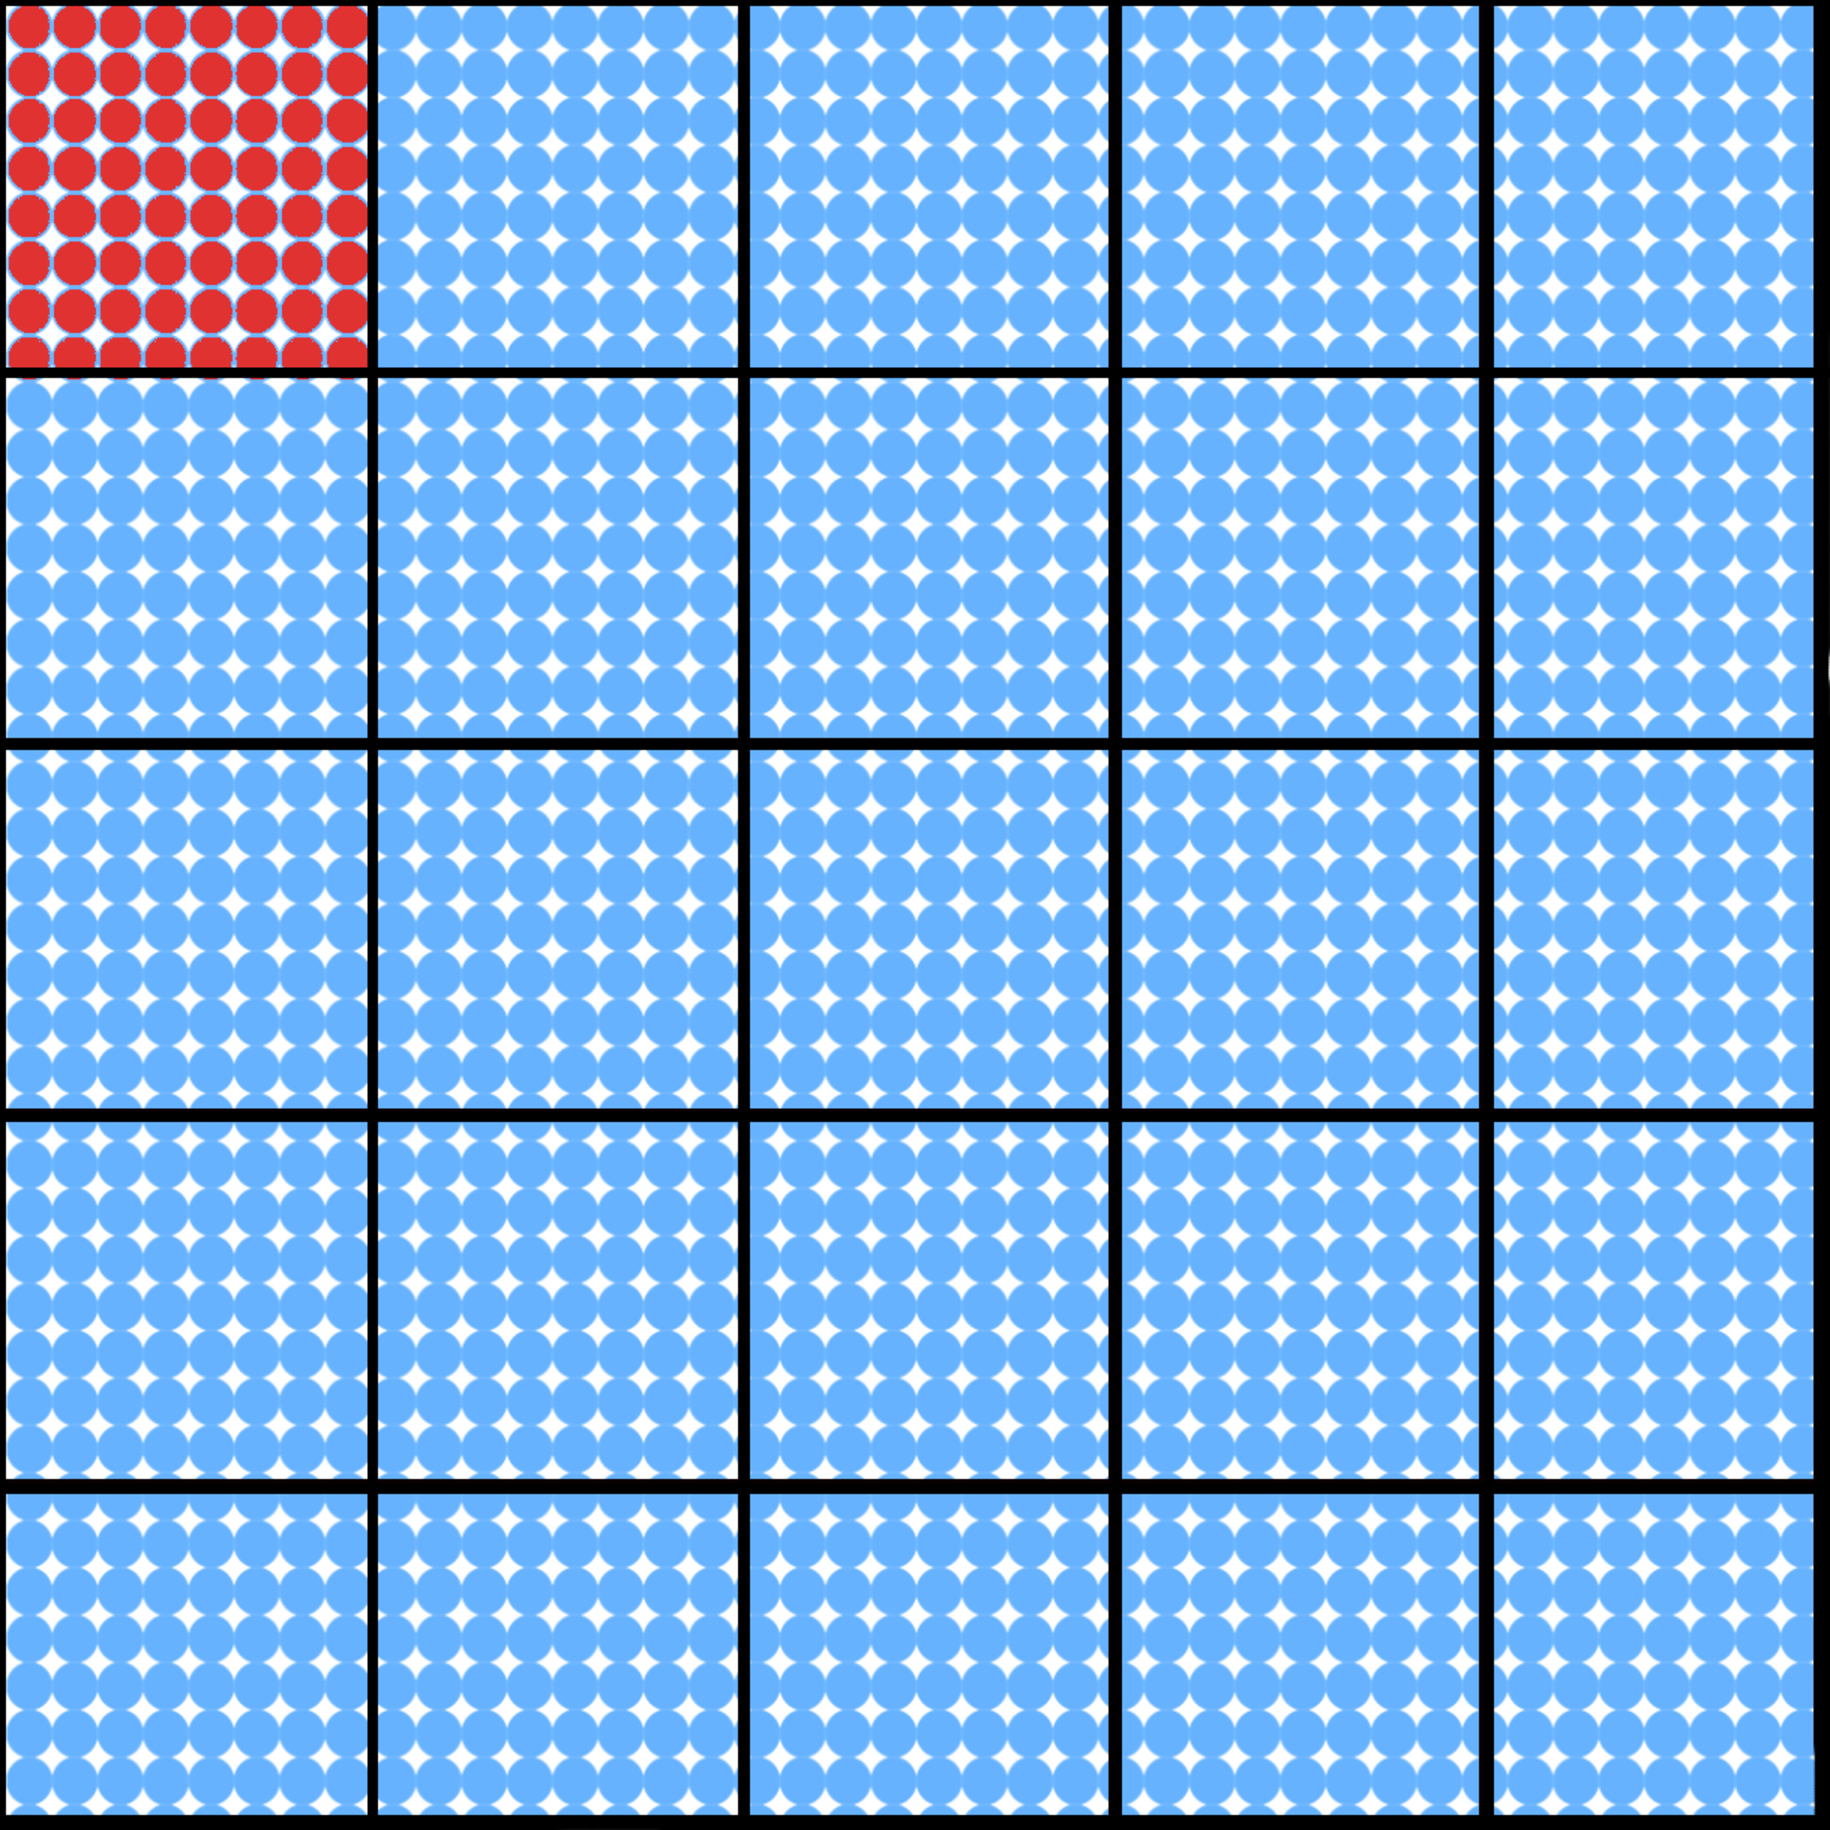
\includegraphics[width=\textwidth]{fig/SVD_tile_1_grid}
    \caption{\label{fig:tile_qr_1} Top corner QR}
  \end{subfigure}
  \hfill
  %%%% 2
  \begin{subfigure}{0.2 \textwidth}
    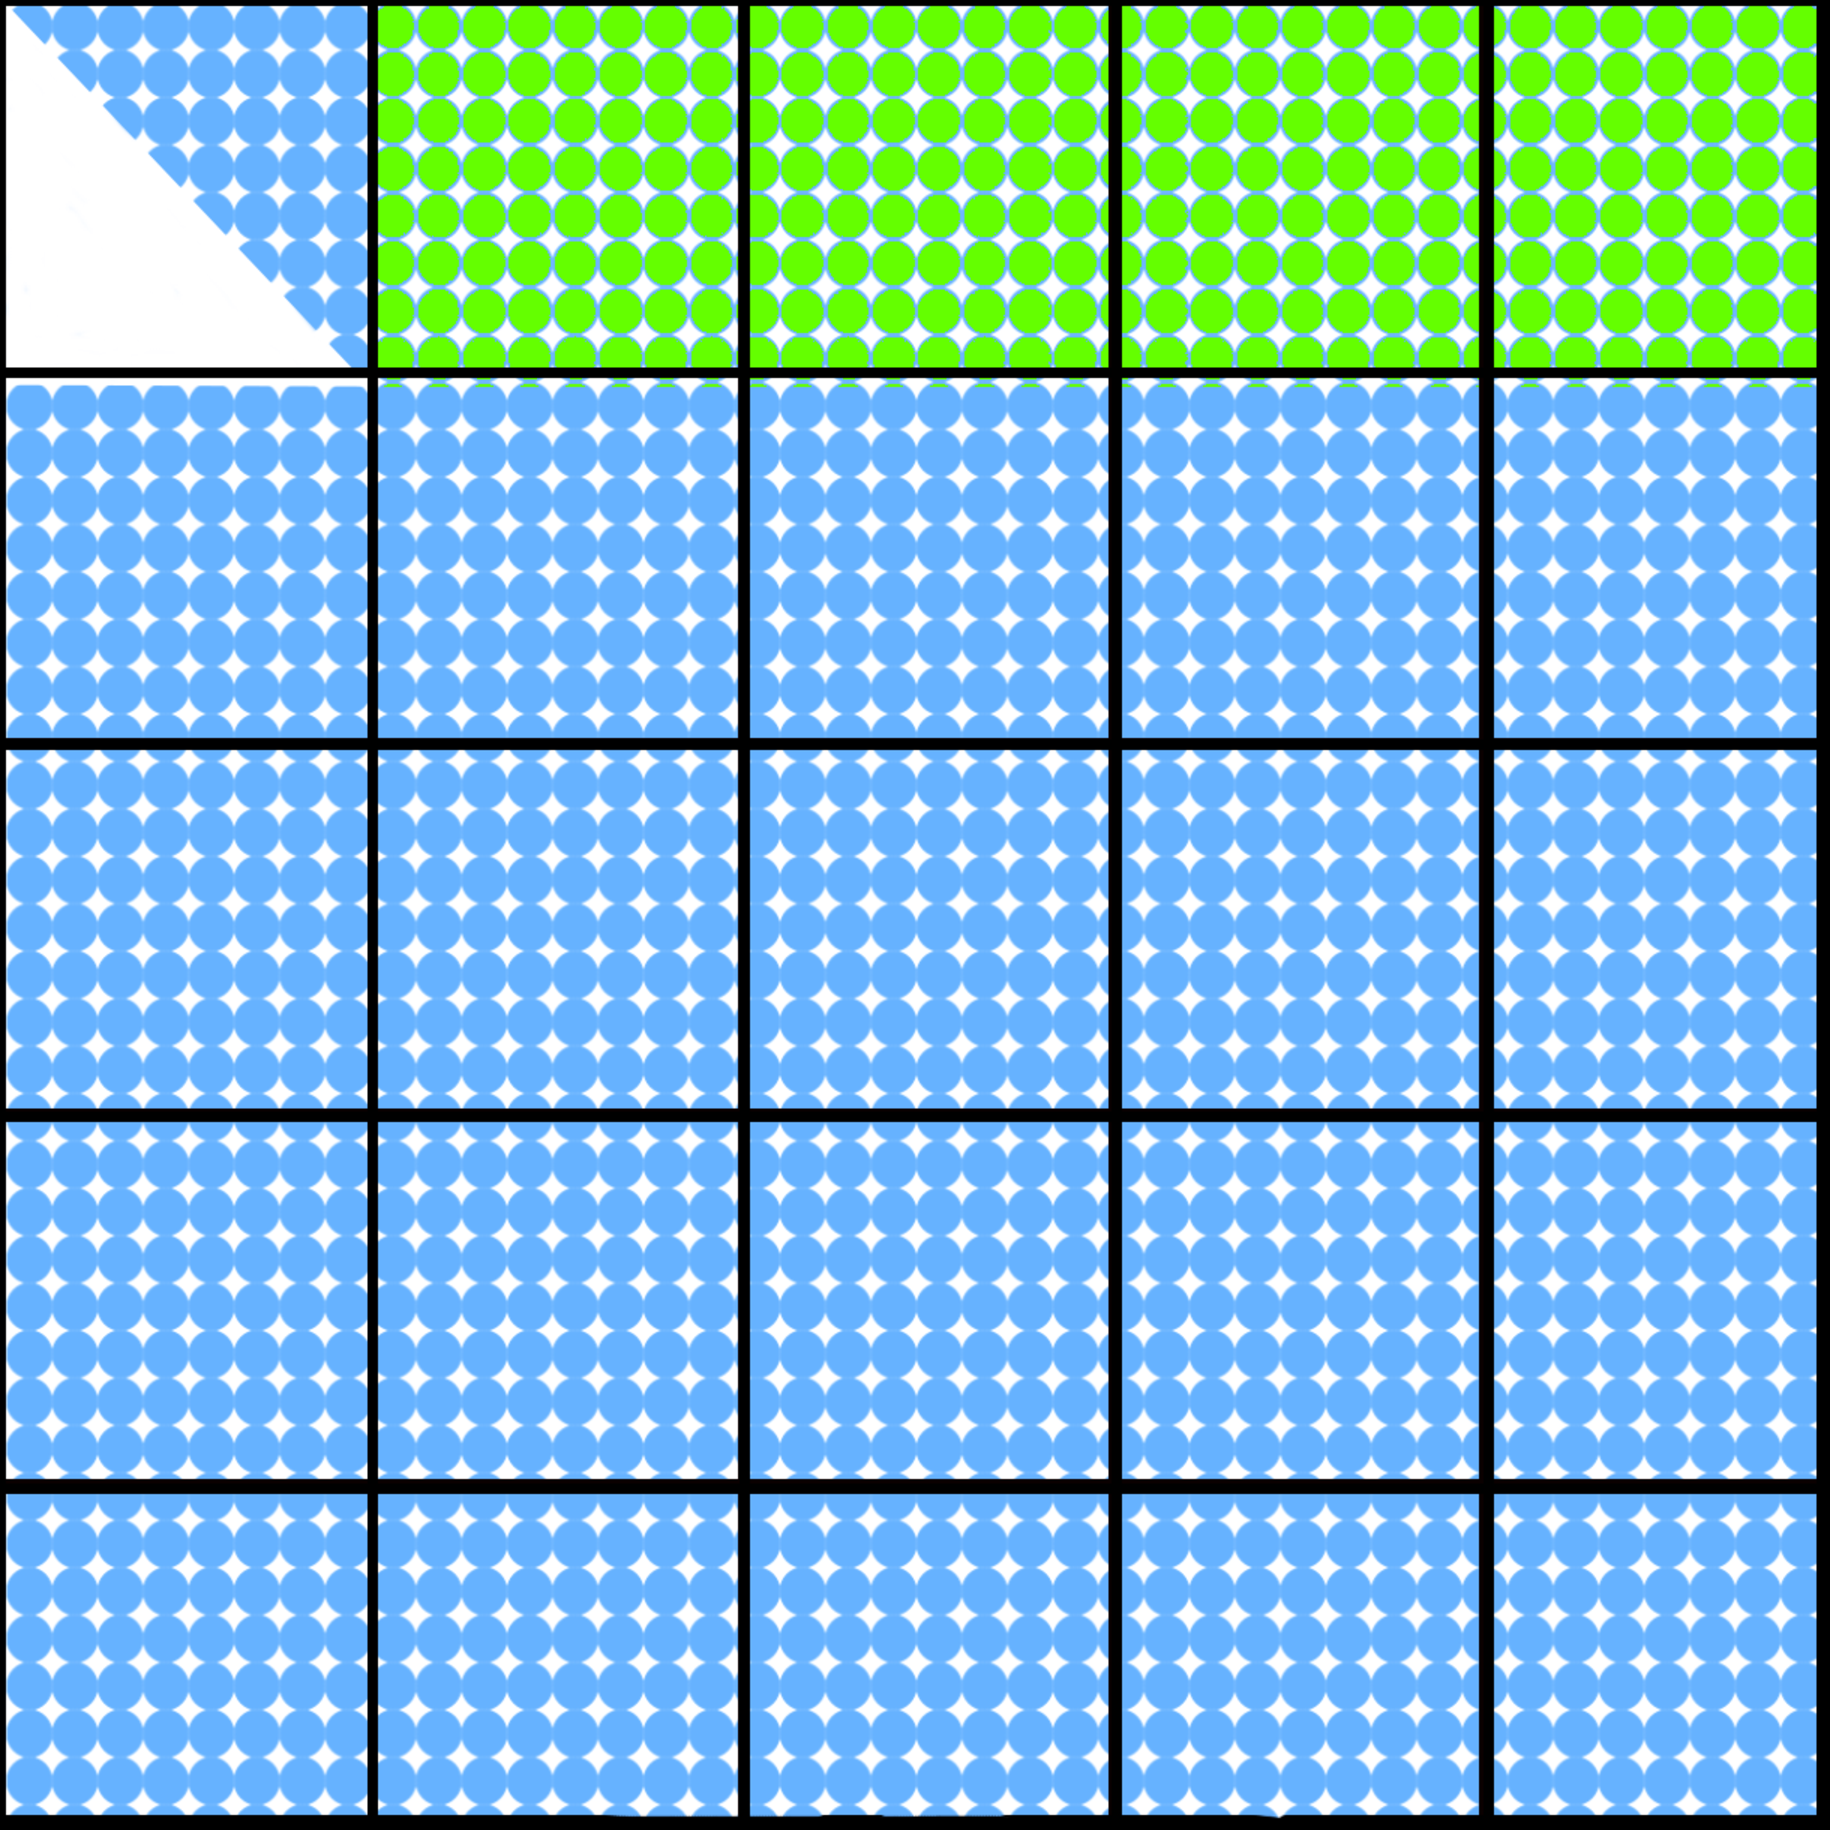
\includegraphics[width=\textwidth]{fig/SVD_tile_2_grid}
    \caption{\label{fig:tile_qr_update_1}Tile-row update}
  \end{subfigure}
  \hfill
  %%%% 3
  \begin{subfigure}{0.2 \textwidth}
    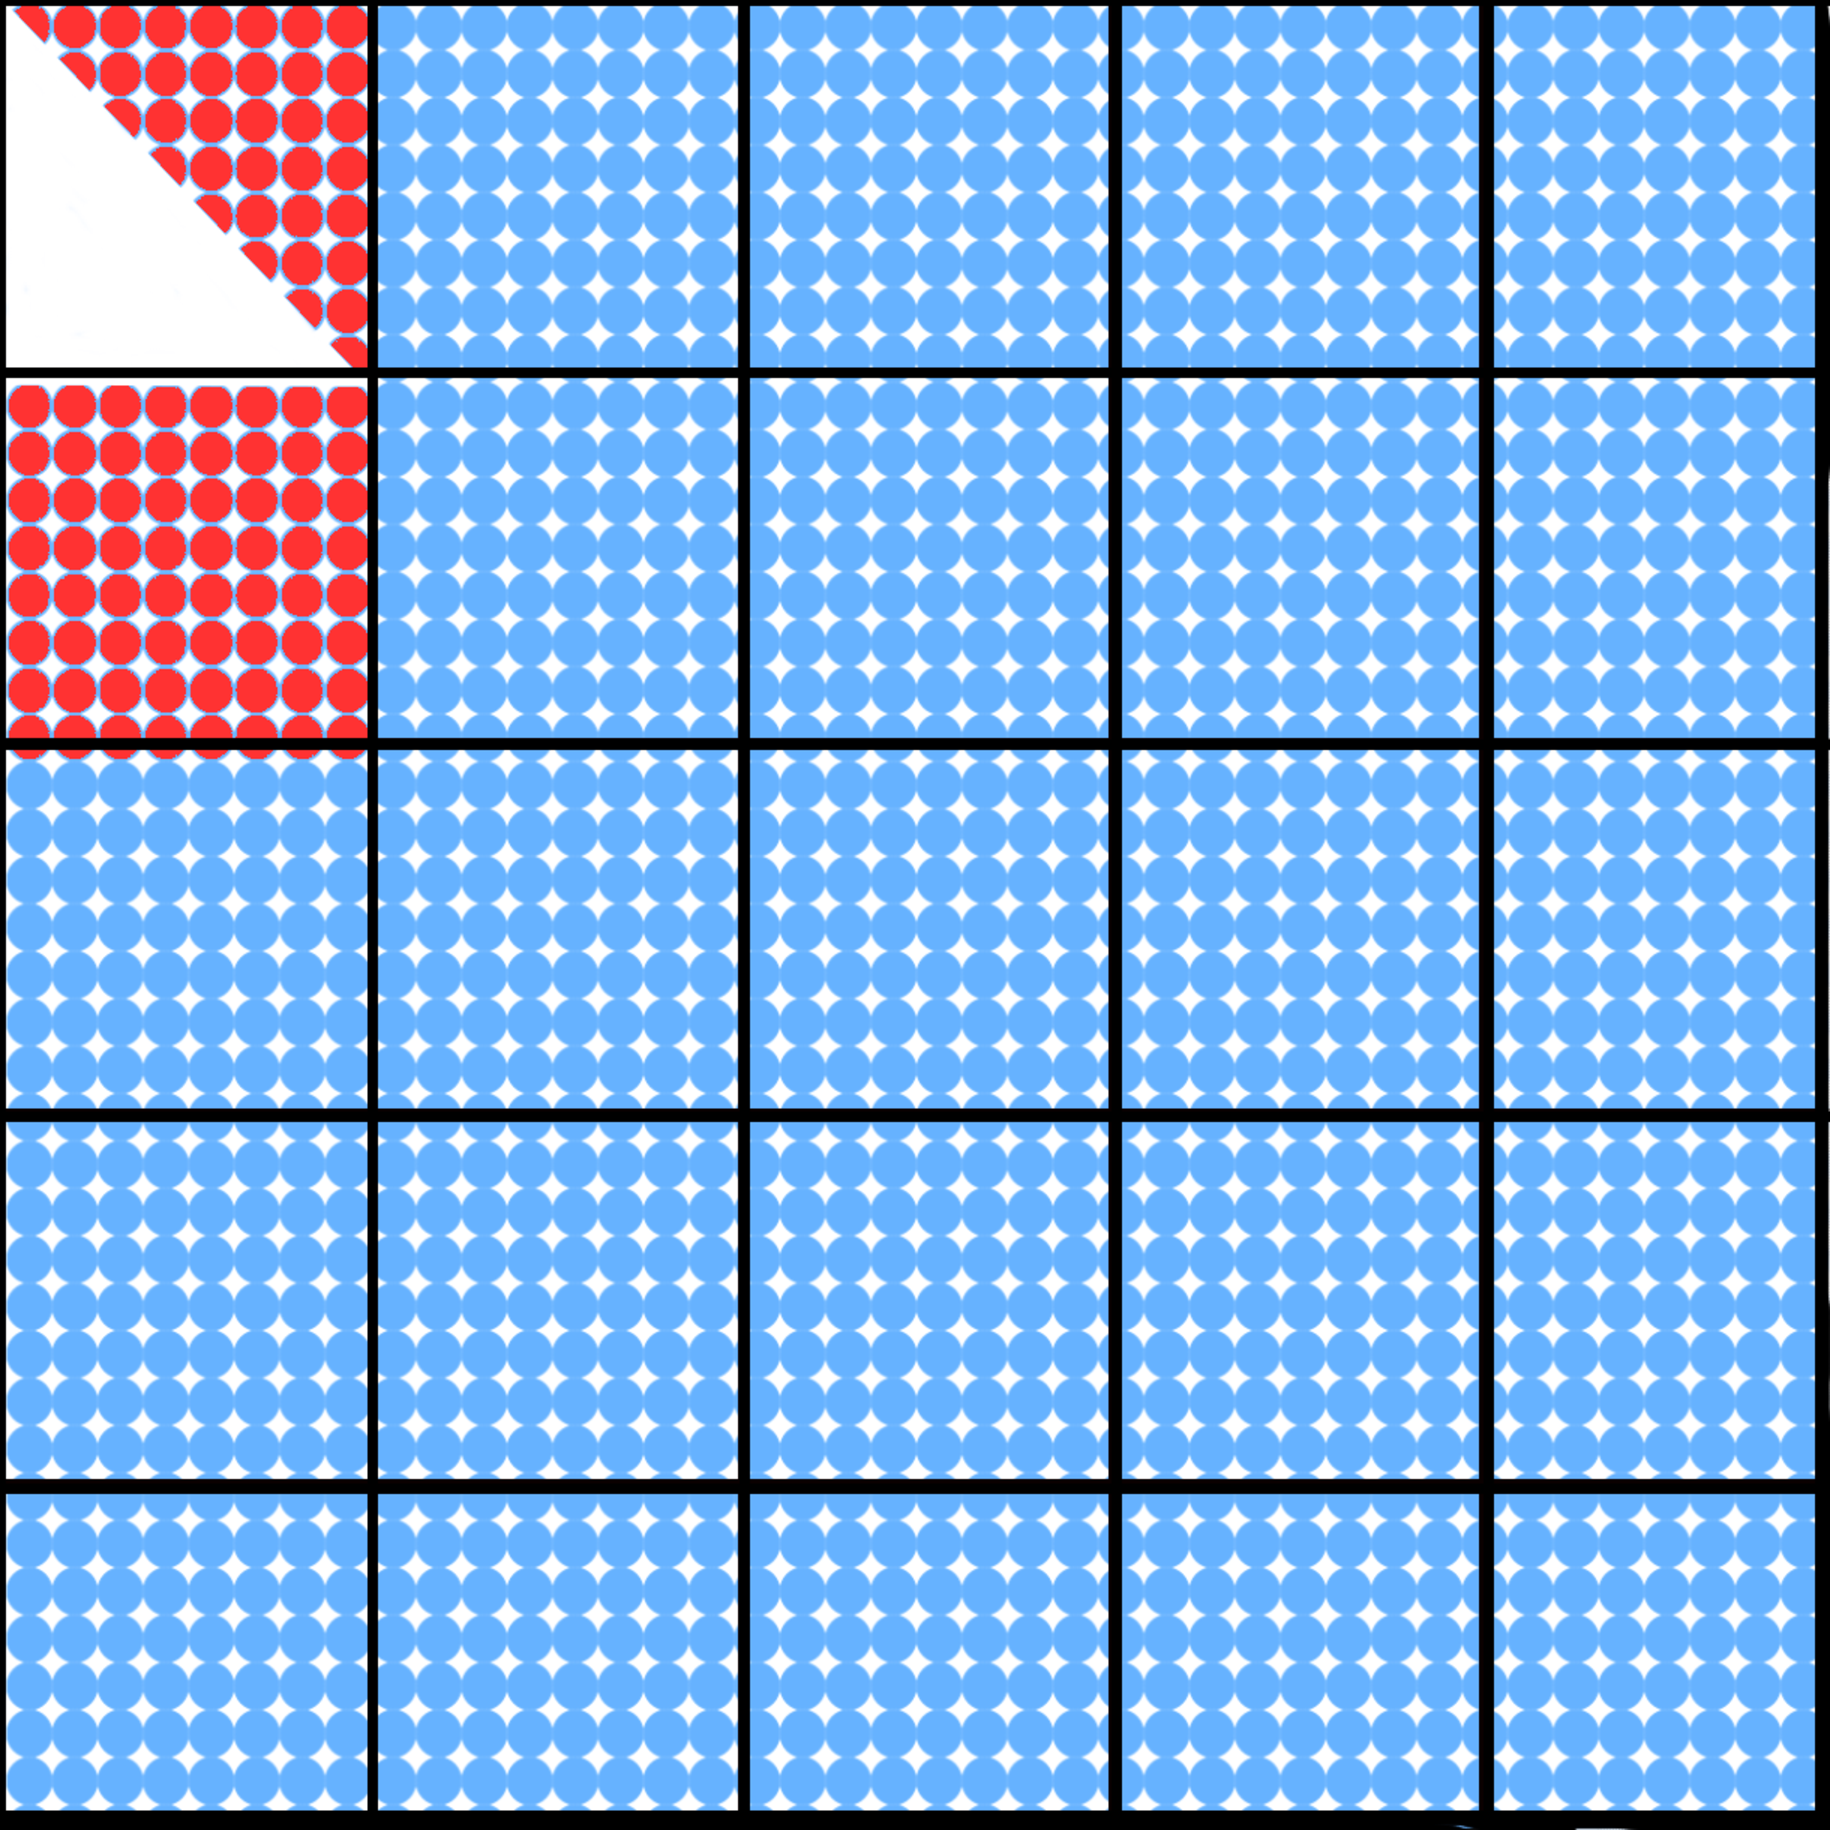
\includegraphics[width=\textwidth]{fig/SVD_tile_3_grid}
    \caption{\label{fig:tile_qr_2}TSQRT}
  \end{subfigure}
  \hfill
  %%%% 4
  \begin{subfigure}{0.2 \textwidth}
    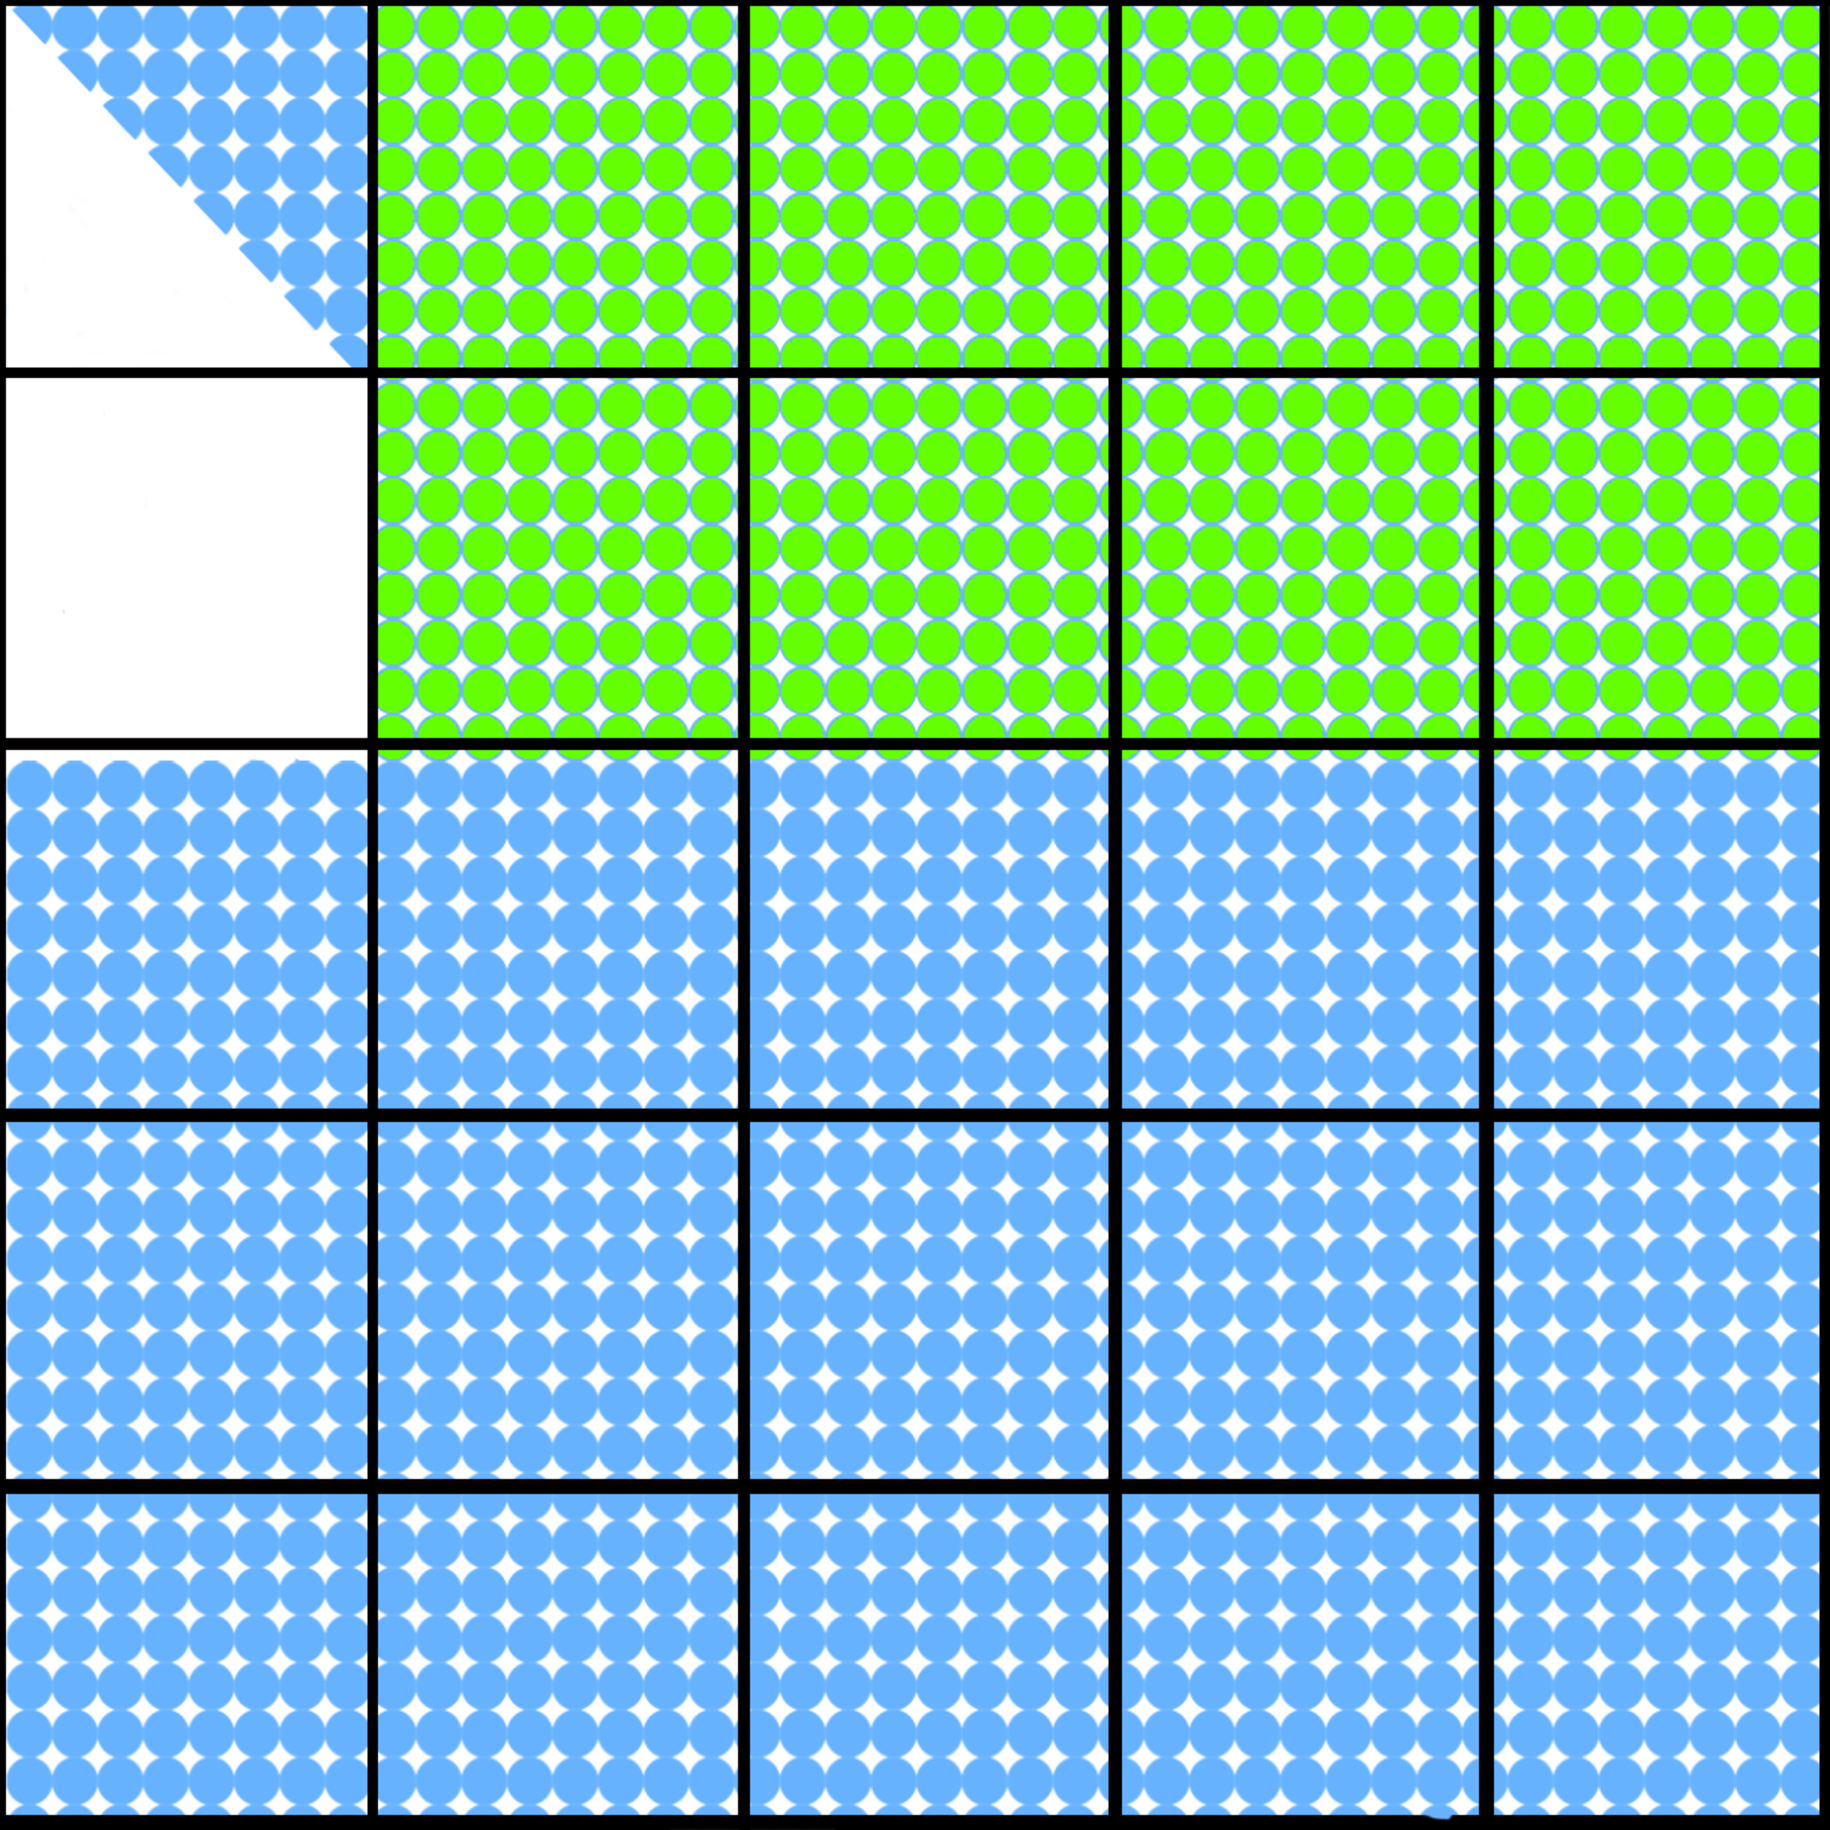
\includegraphics[width=\textwidth]{fig/SVD_tile_4_grid}
    \caption{\label{fig:tile_qr_update_2}Tile-rows update}
  \end{subfigure}
  \hfill
  %%%% 5
  \begin{subfigure}{0.2 \textwidth}
    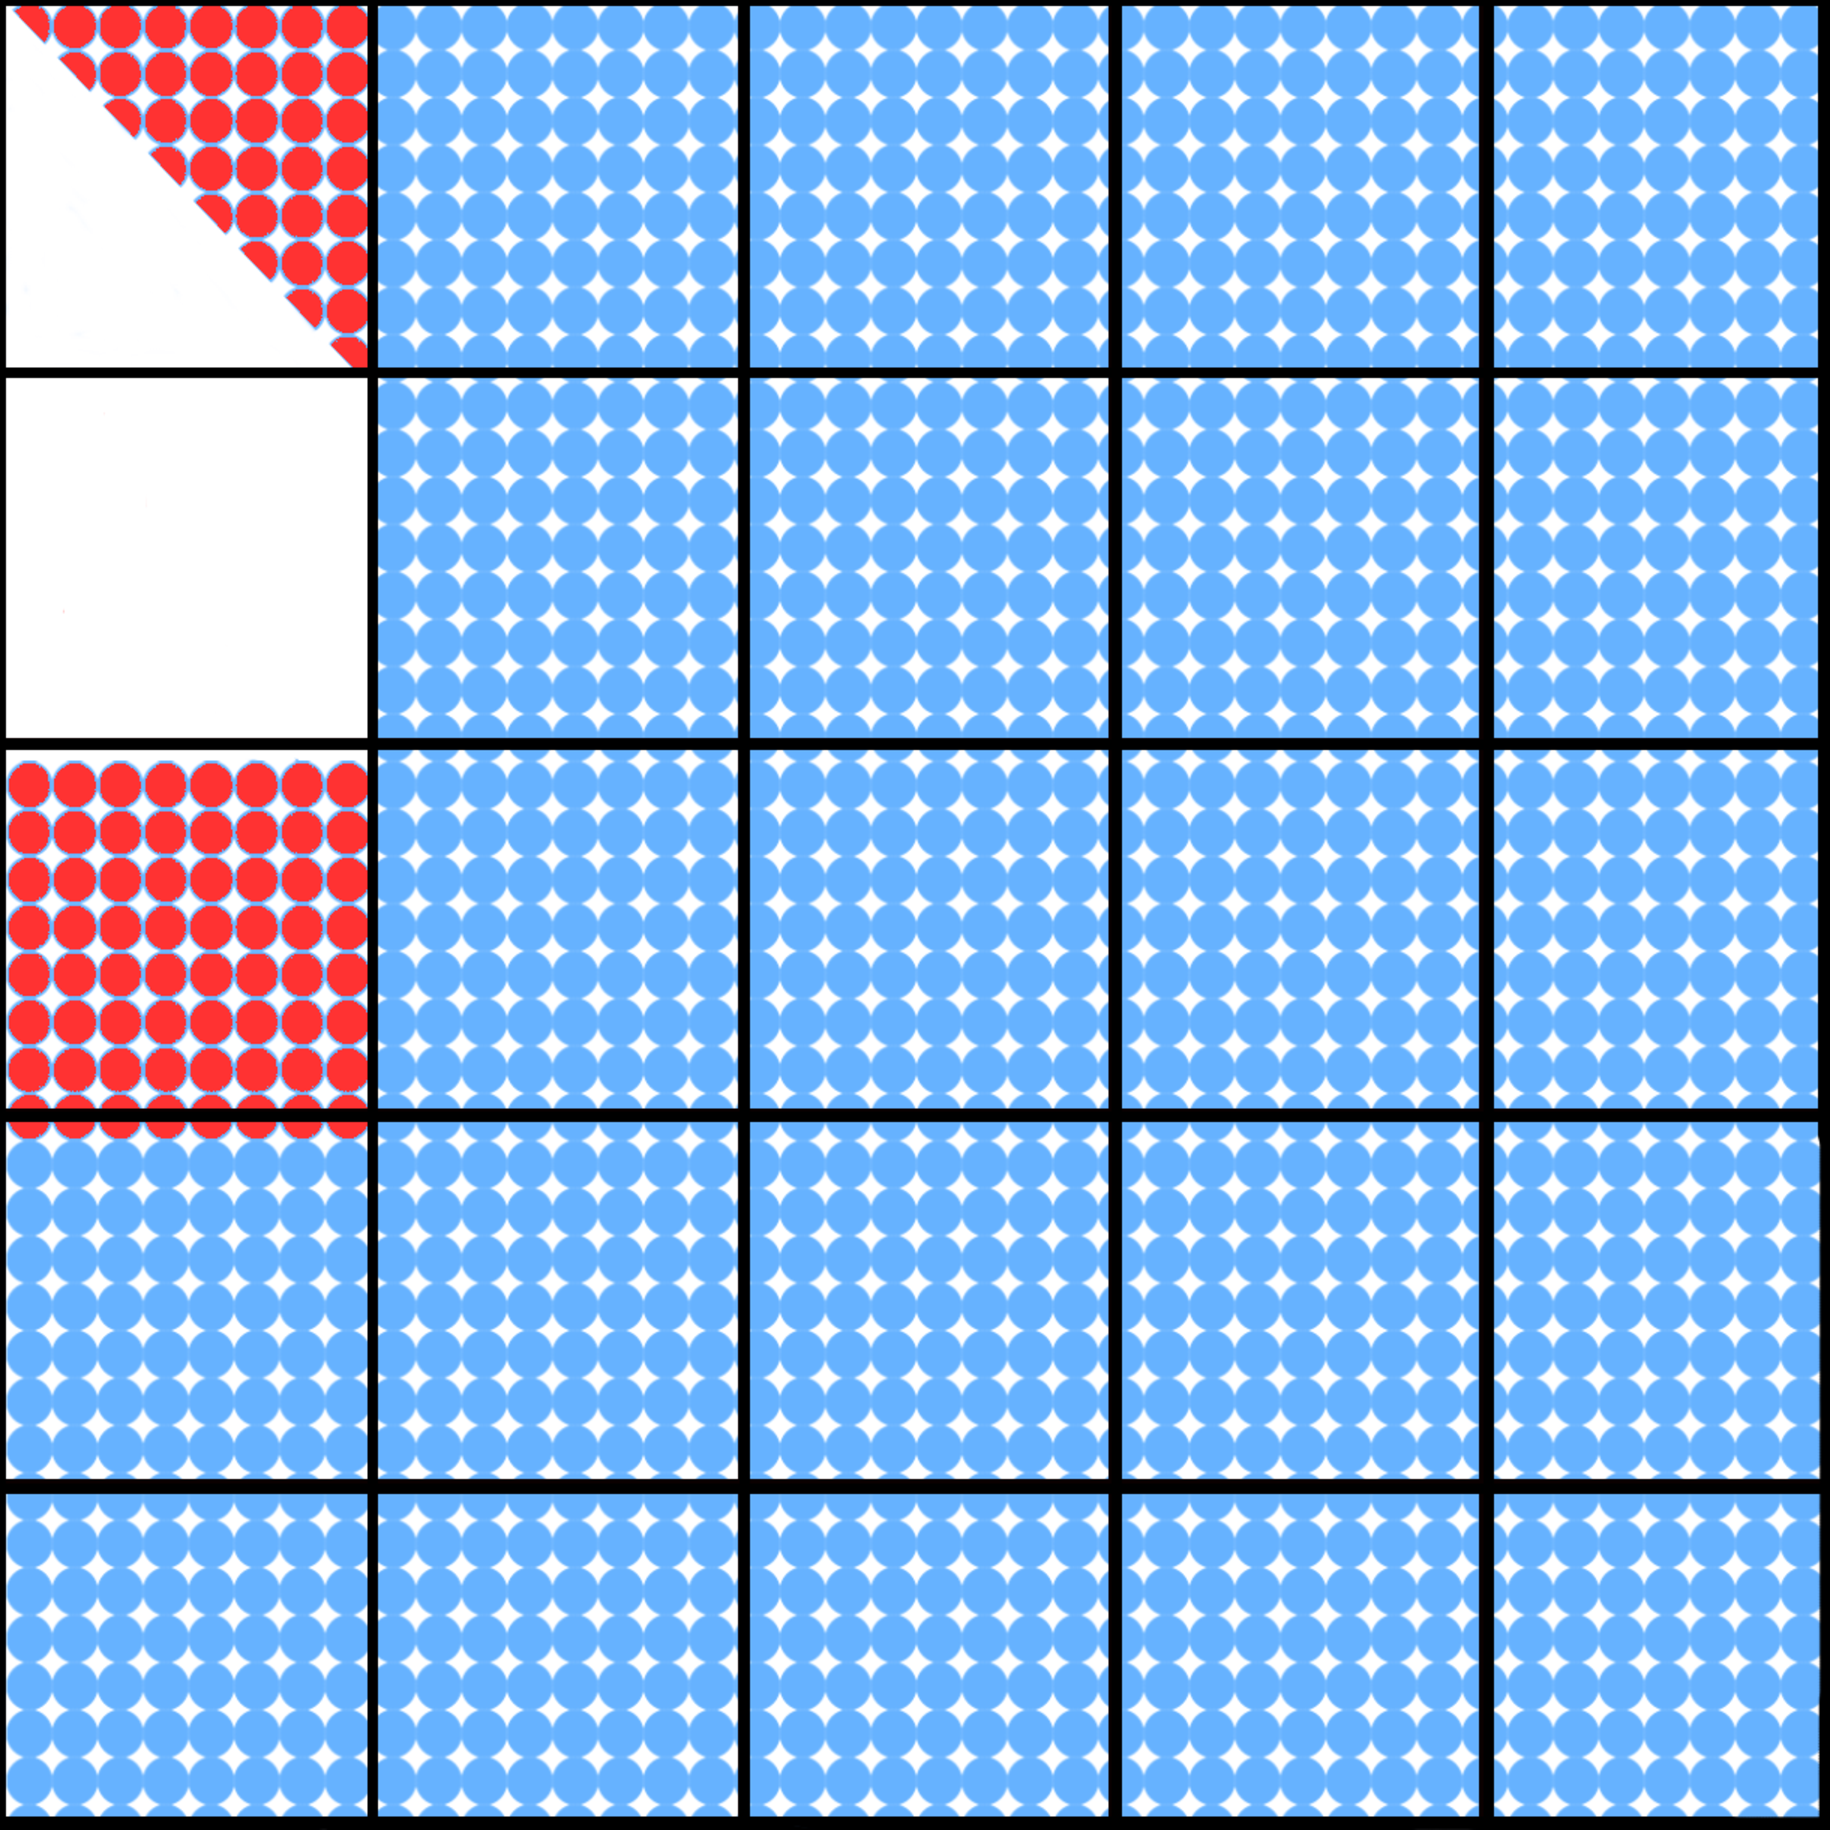
\includegraphics[width=\textwidth]{fig/SVD_tile_5_grid}
    \caption{\label{fig:tile_qr_3}TSQRT}
  \end{subfigure}
  \hfill
  %%%% 6
  \begin{subfigure}{0.2 \textwidth}
    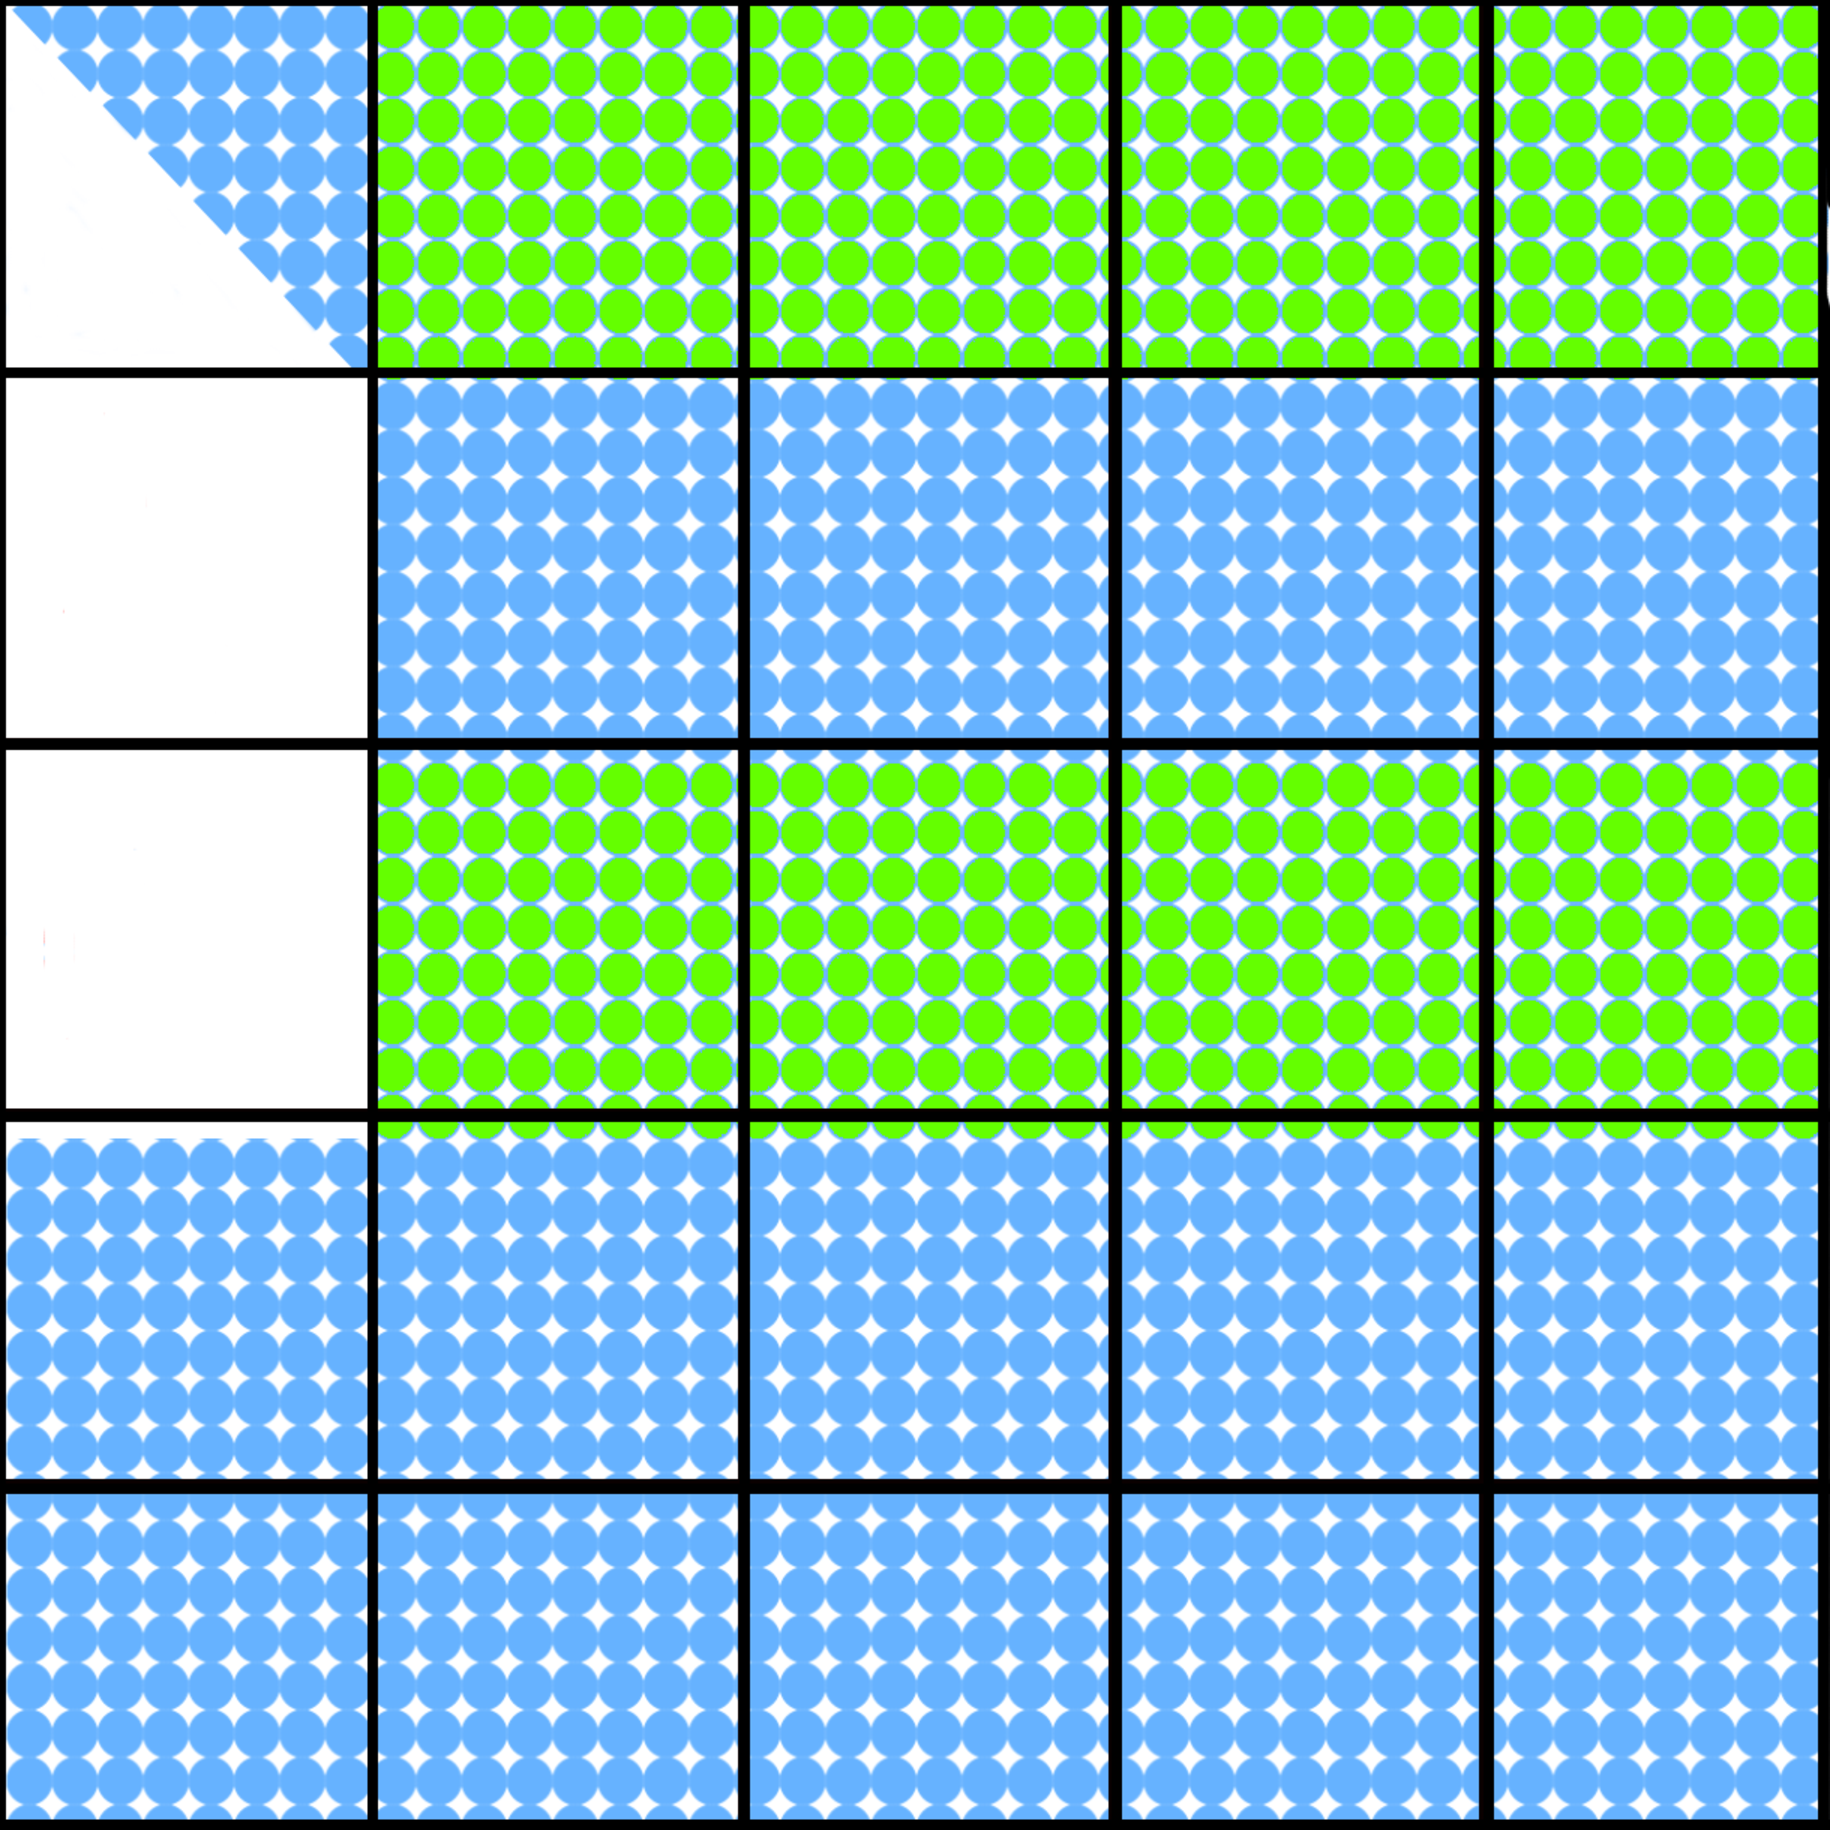
\includegraphics[width=\textwidth]{fig/SVD_tile_6_grid}
    \caption{\label{fig:tile_qr_update_3}Tile-rows update}
  \end{subfigure}
  \hfill
  %%%% 7
  \begin{subfigure}{0.2 \textwidth}
    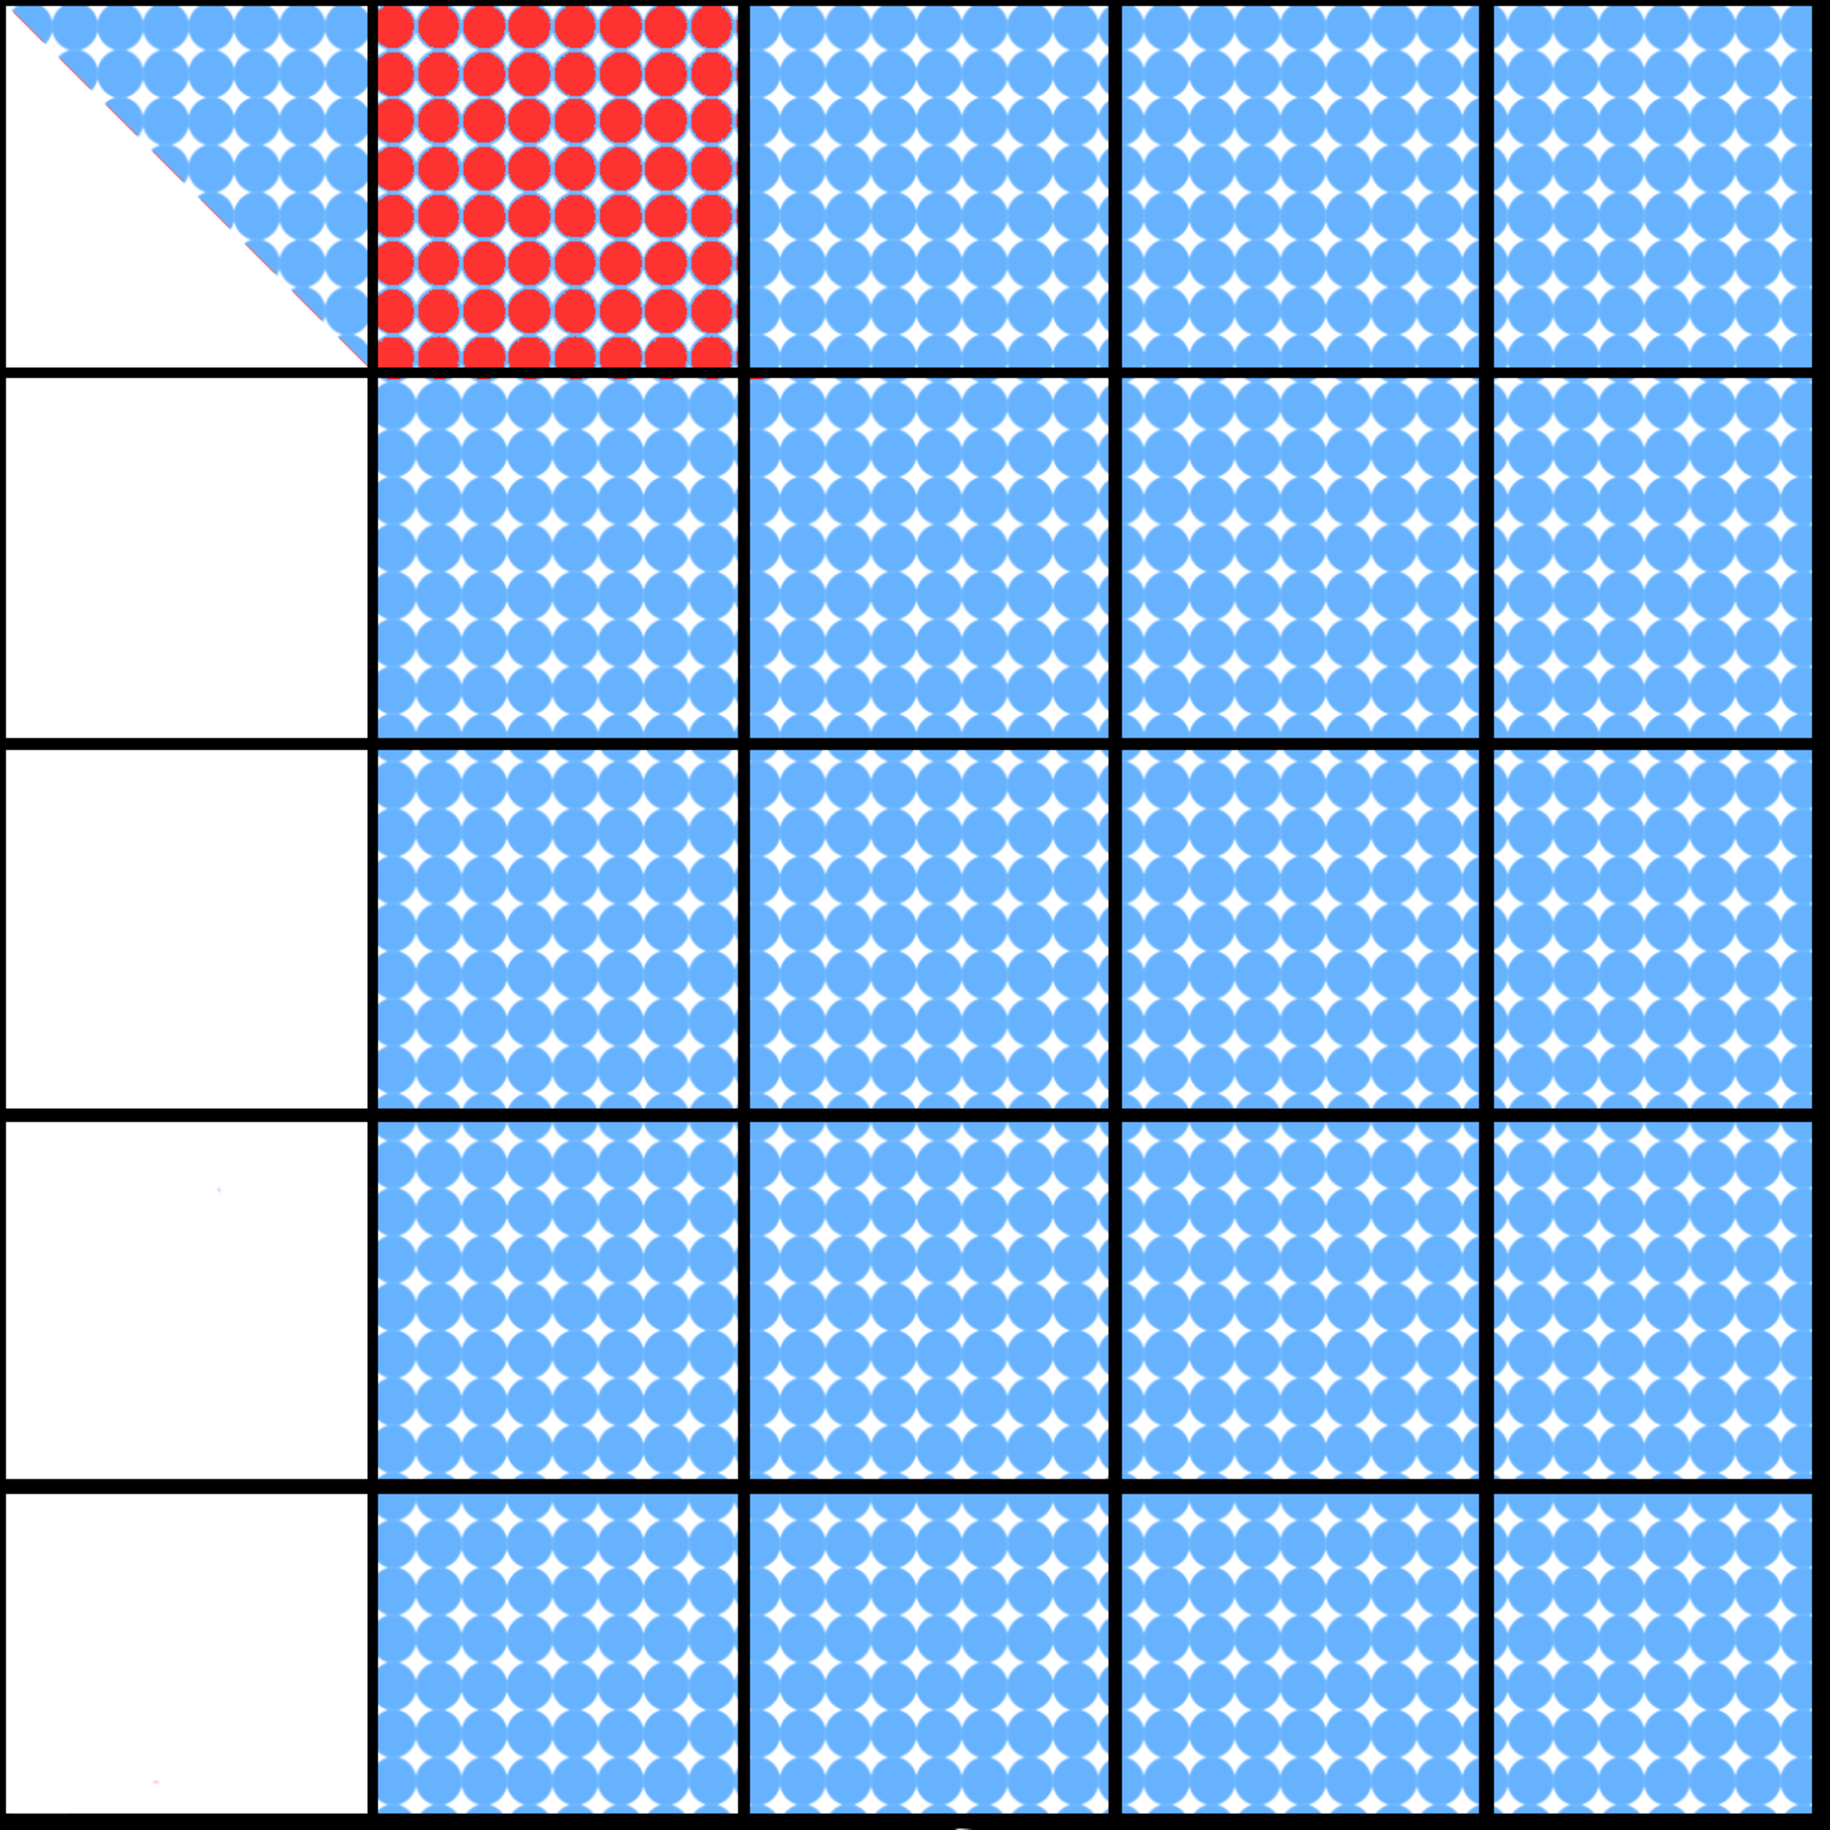
\includegraphics[width=\textwidth]{fig/SVD_tile_7_grid}
      \caption{\label{fig:tile_lq_2}LQ }
  \end{subfigure}
  \hfill
  %%%% 8
  \begin{subfigure}{0.2 \textwidth}
    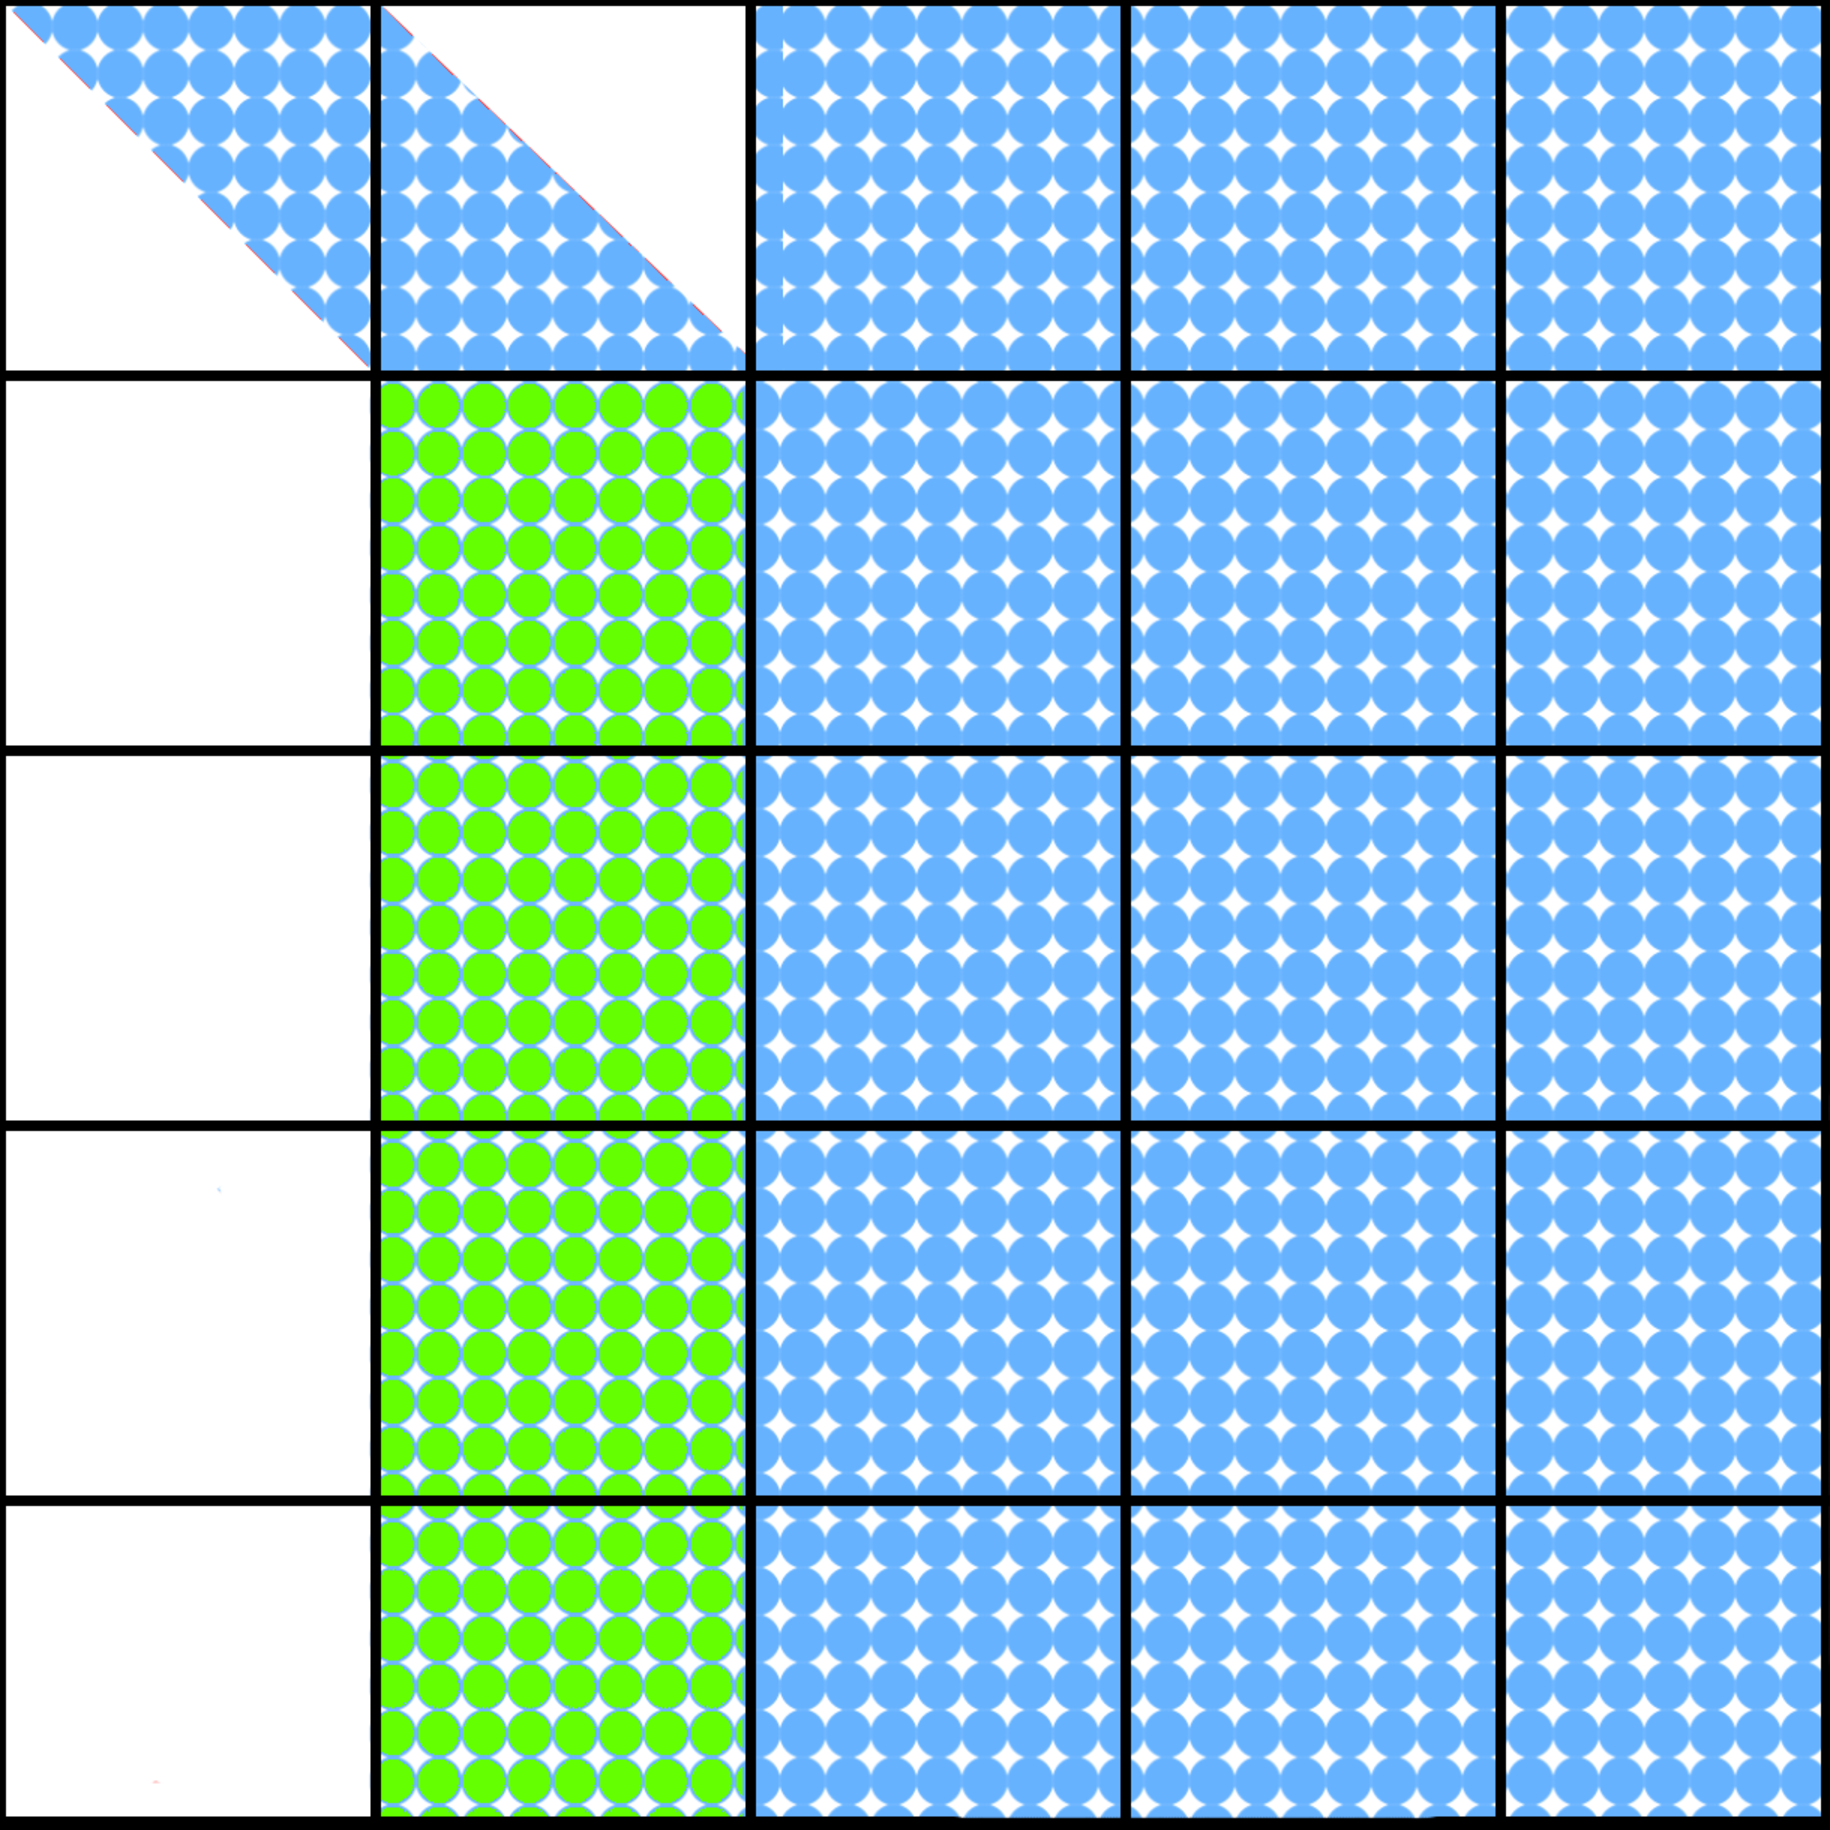
\includegraphics[width=\textwidth]{fig/SVD_tile_8_grid}
      \caption{\label{fig:tile_lq_update_2}Panel update}
  \end{subfigure}
  \hfill
  %%%% 9
  \begin{subfigure}{0.2 \textwidth}
    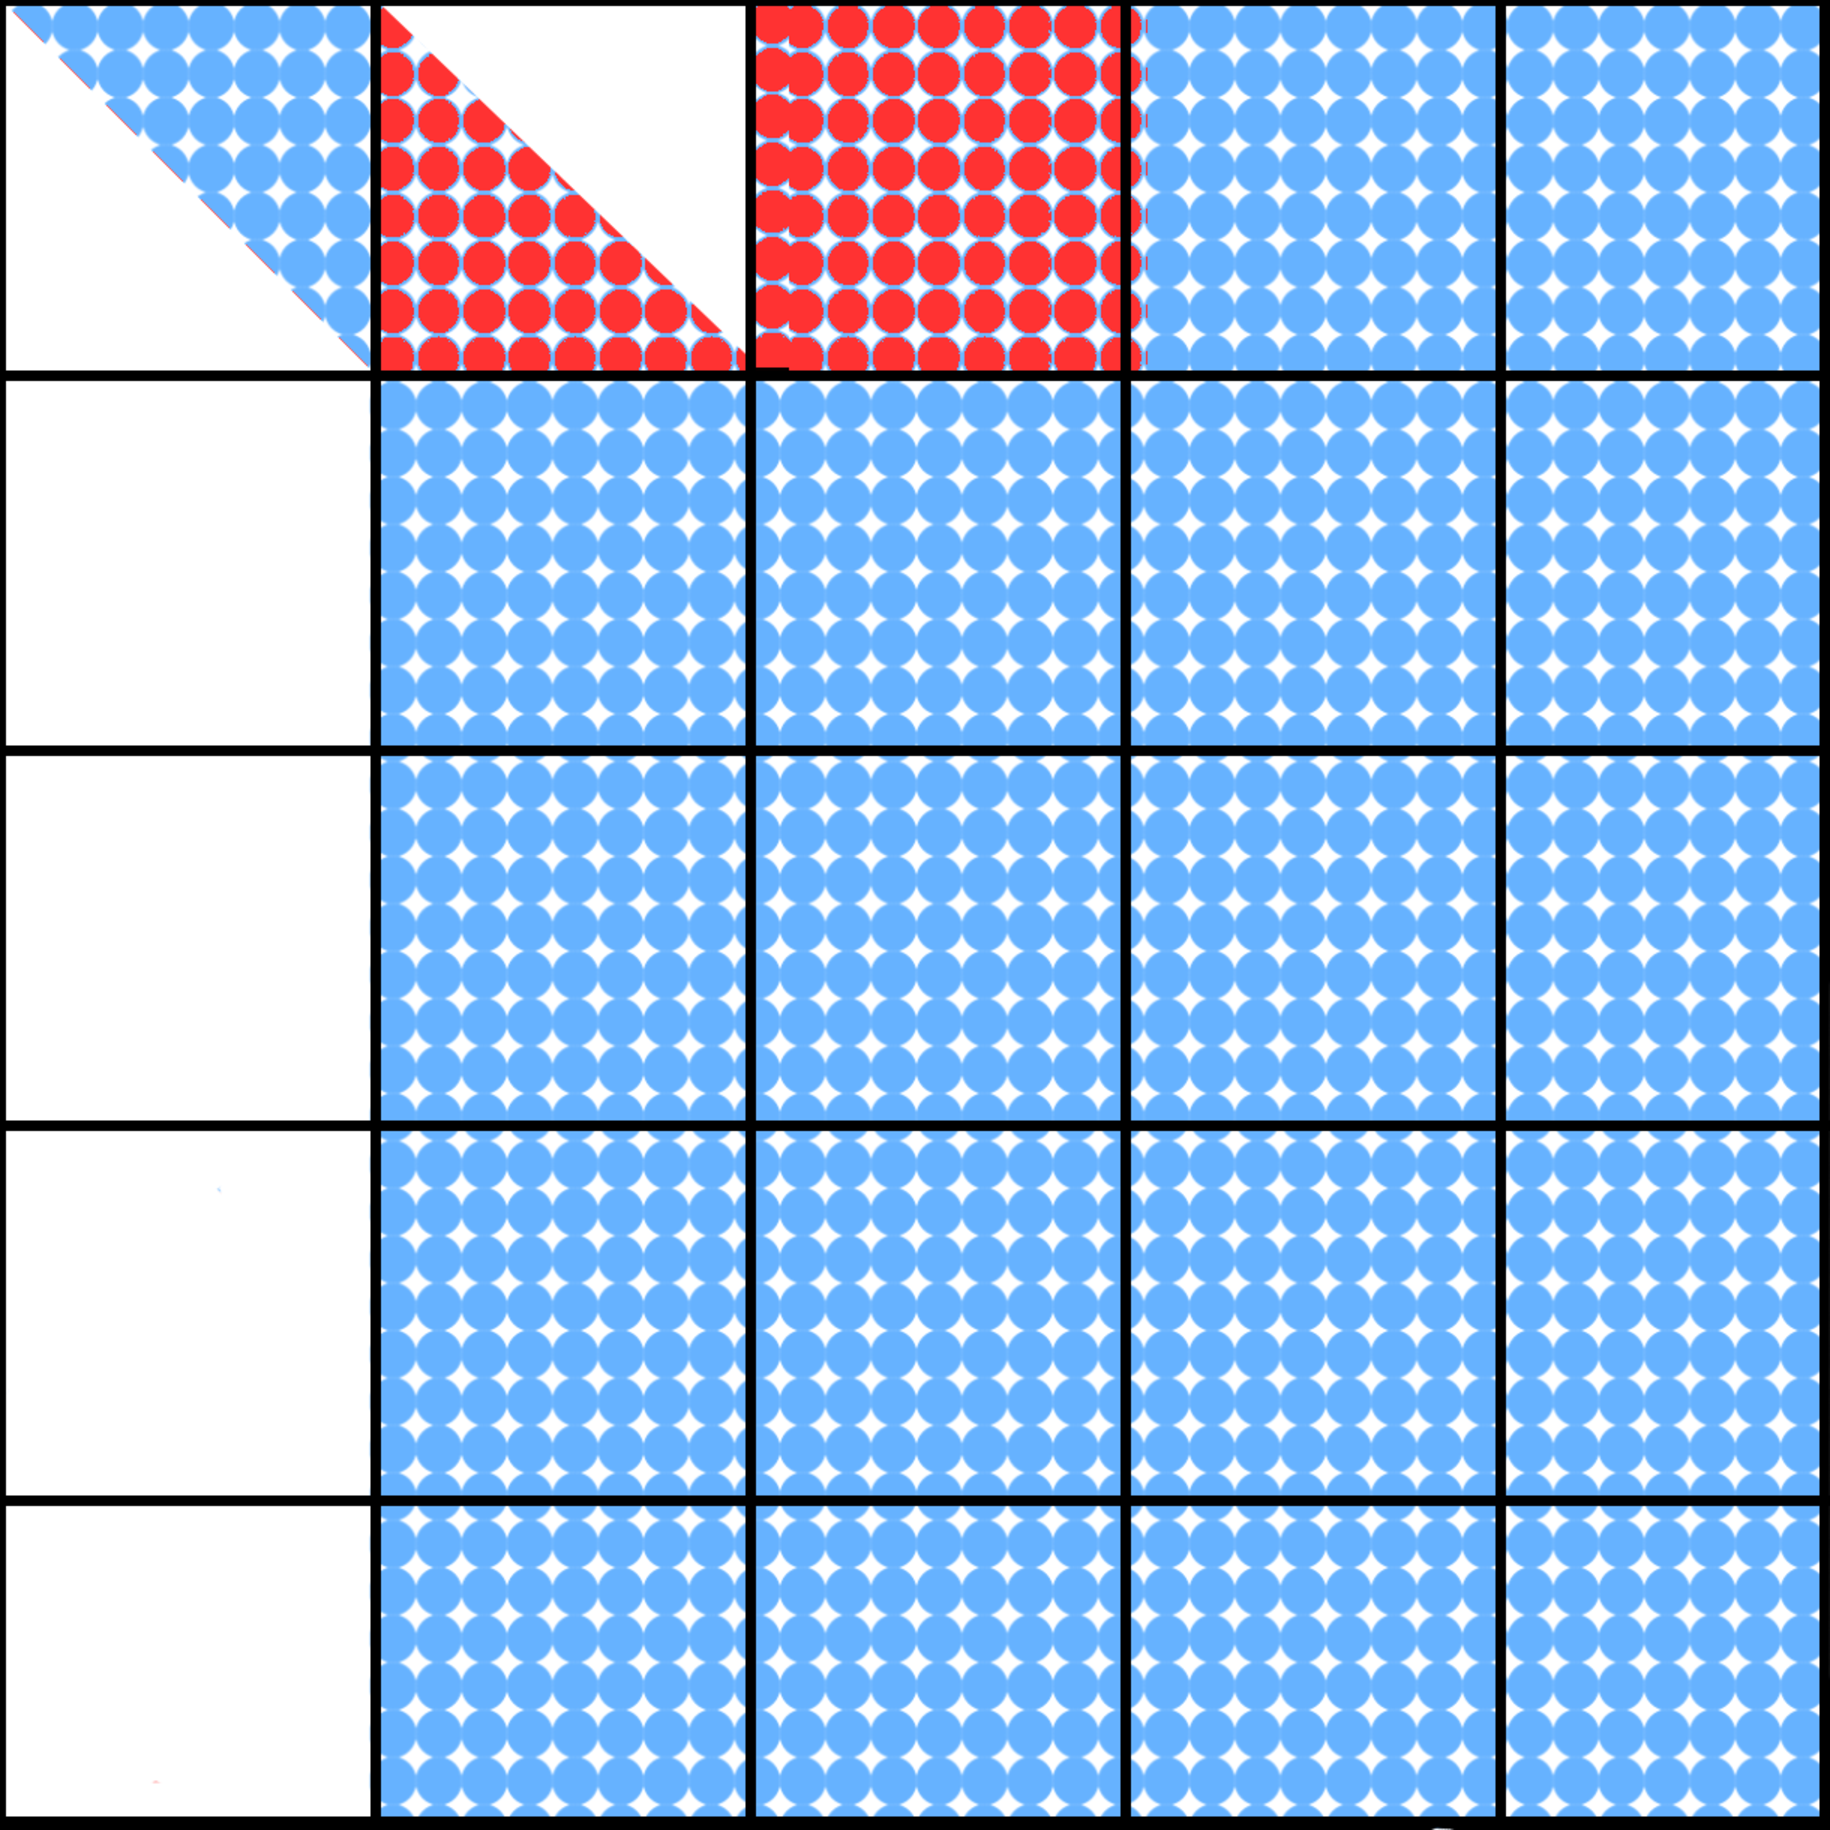
\includegraphics[width=\textwidth]{fig/SVD_tile_9_grid}
    \caption{\label{fig:tile_lq_update_2}TSLQT}
  \end{subfigure}
  \hfill
  %%%% 10
  \begin{subfigure}{0.2 \textwidth}
    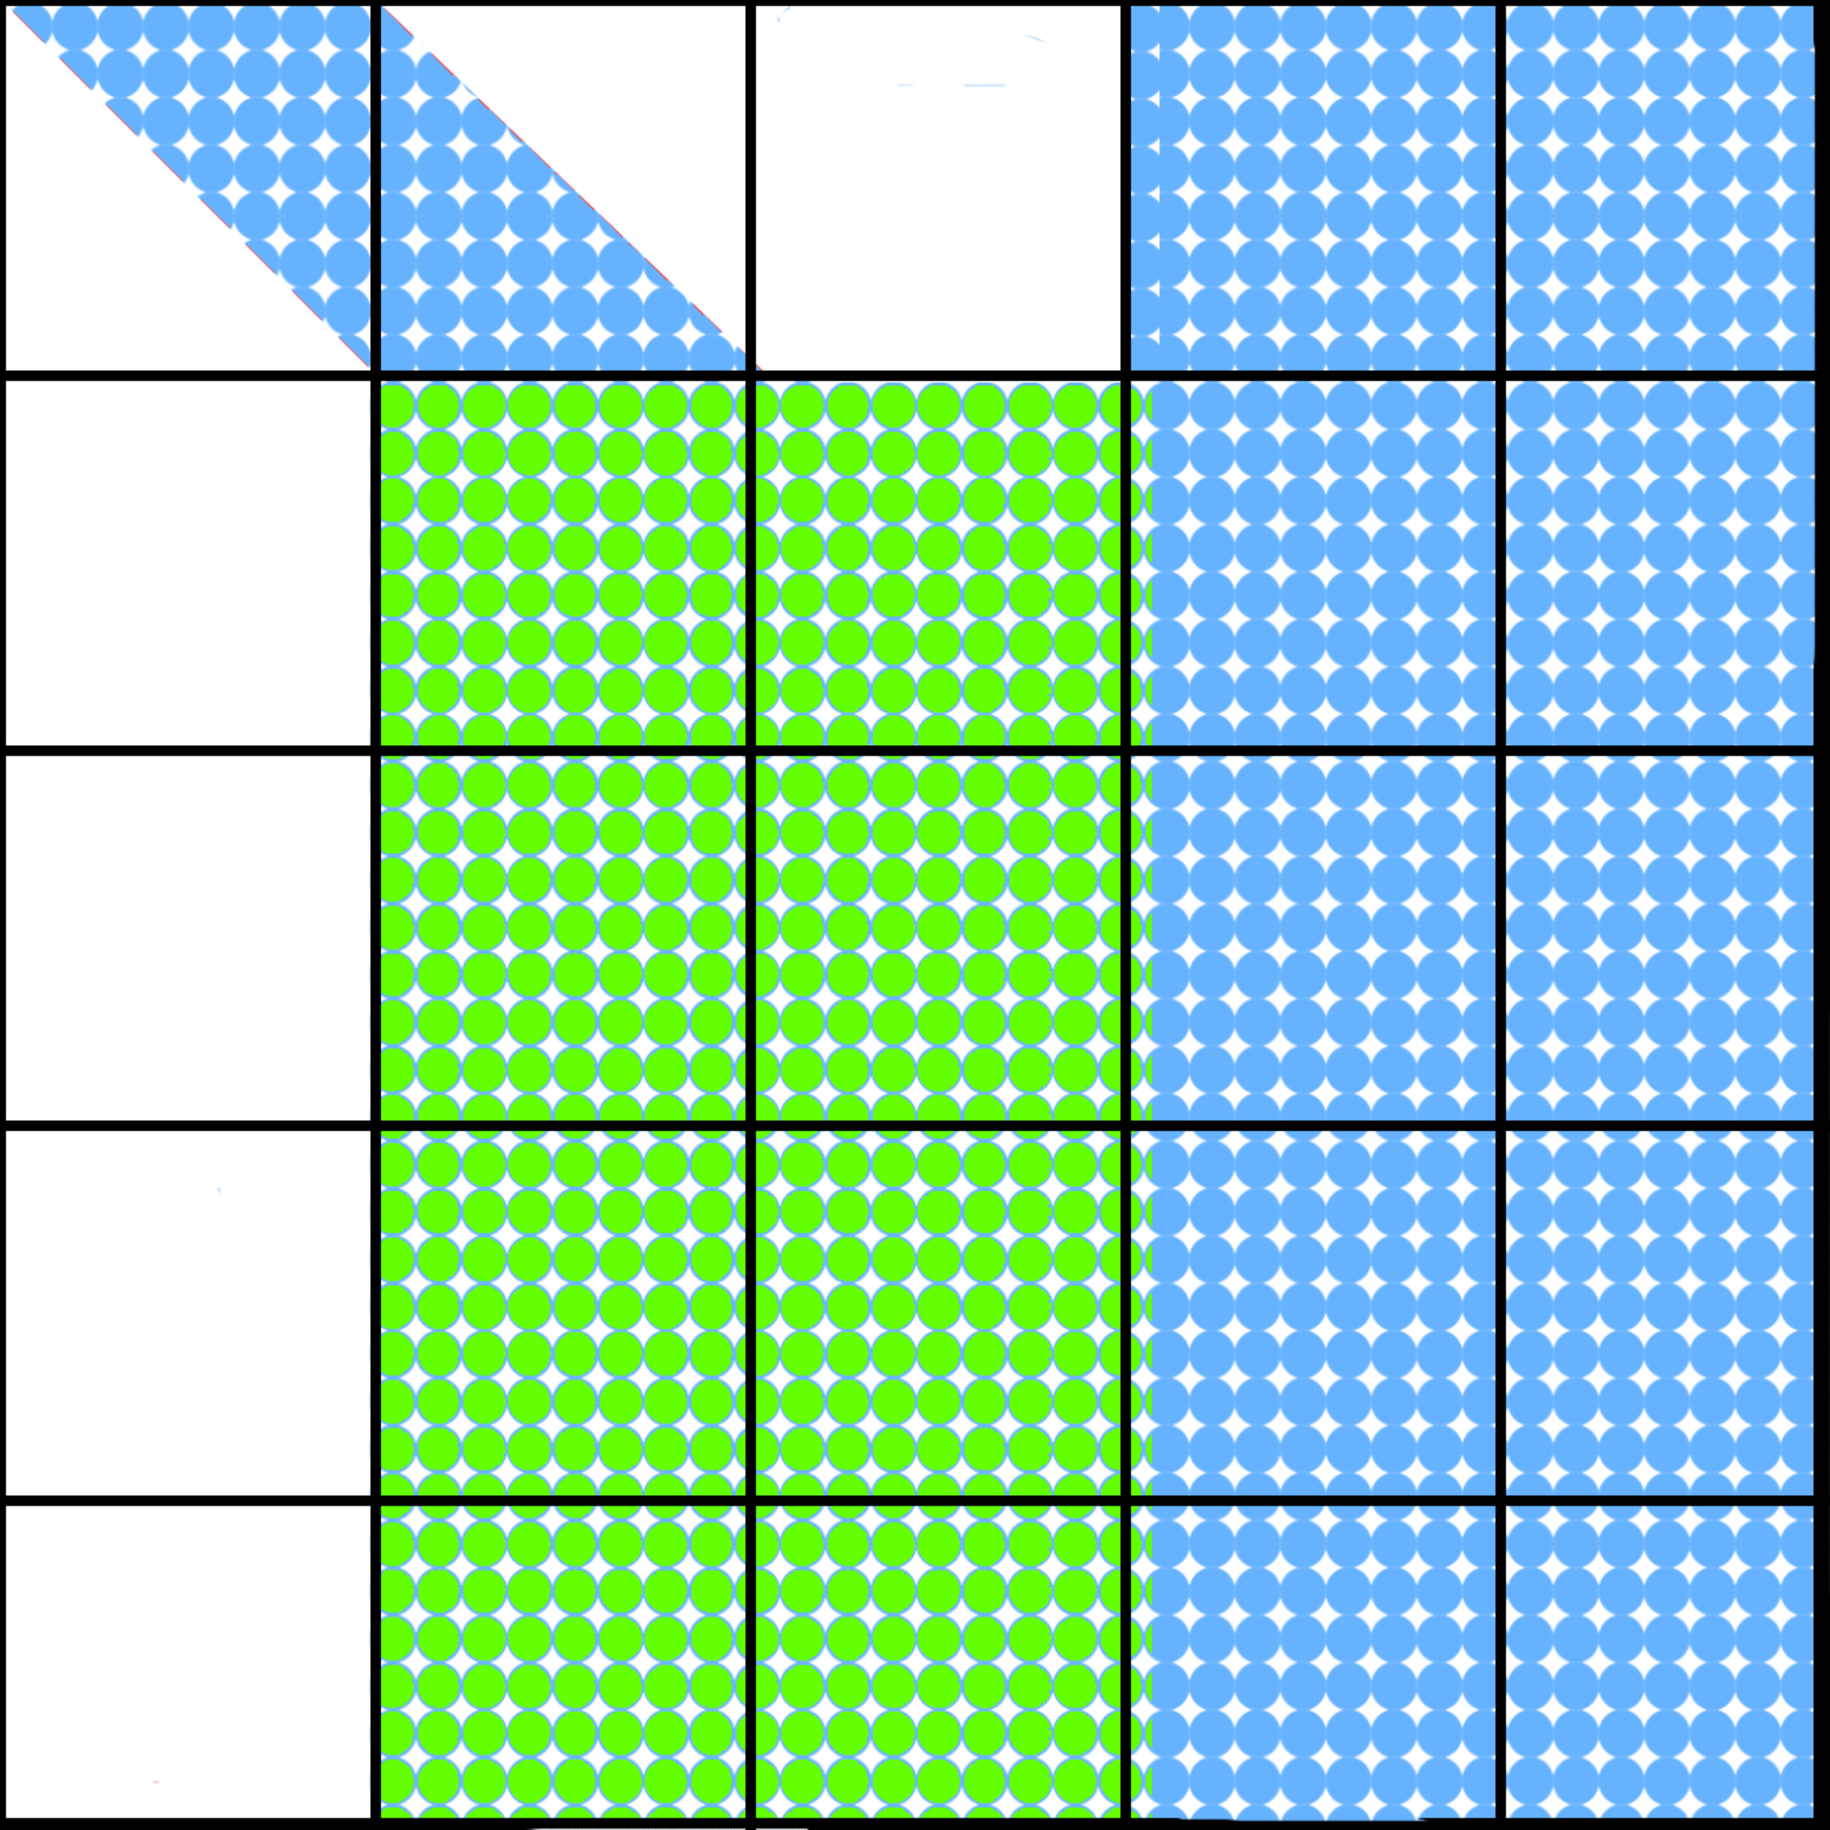
\includegraphics[width=\textwidth]{fig/SVD_tile_10_grid}
    \caption{\label{fig:tile_lq_update_2}Panel update}
  \end{subfigure}
  \hfill
  %%%% 11
  \begin{subfigure}{0.2 \textwidth}
    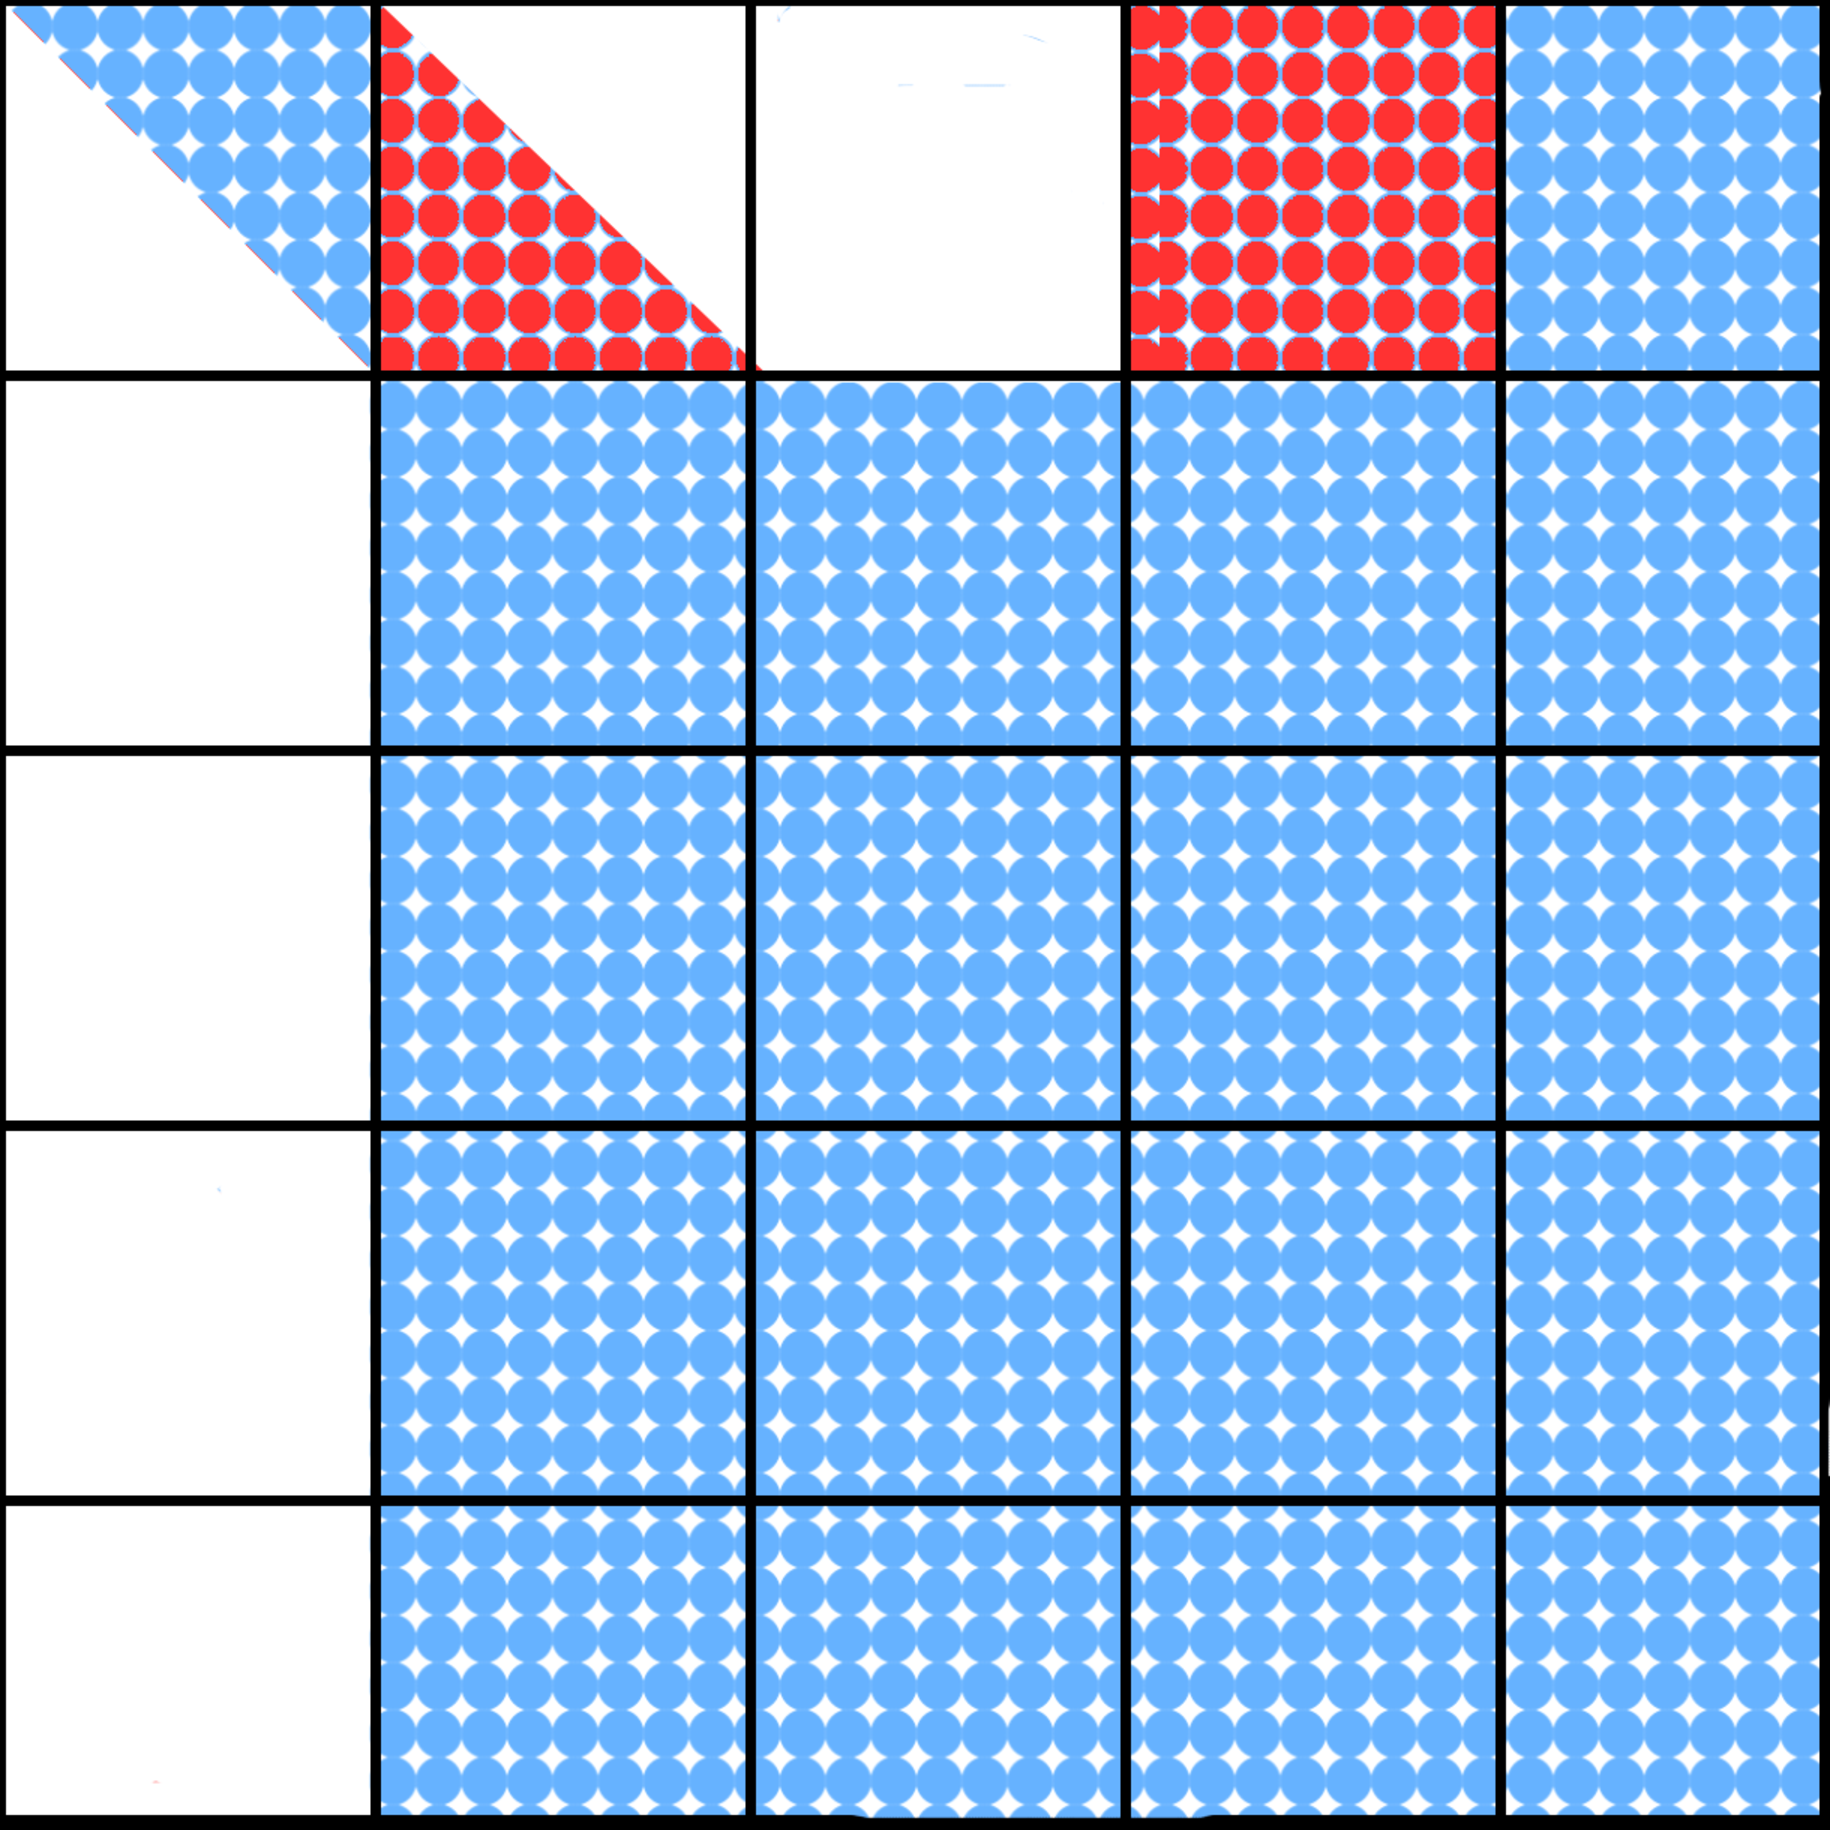
\includegraphics[width=\textwidth]{fig/SVD_tile_11_grid}
    \caption{\label{fig:tile_lq_update_2}TSLQT}
  \end{subfigure}
  \hfill
  %%%% 8
  \begin{subfigure}{0.2 \textwidth}
    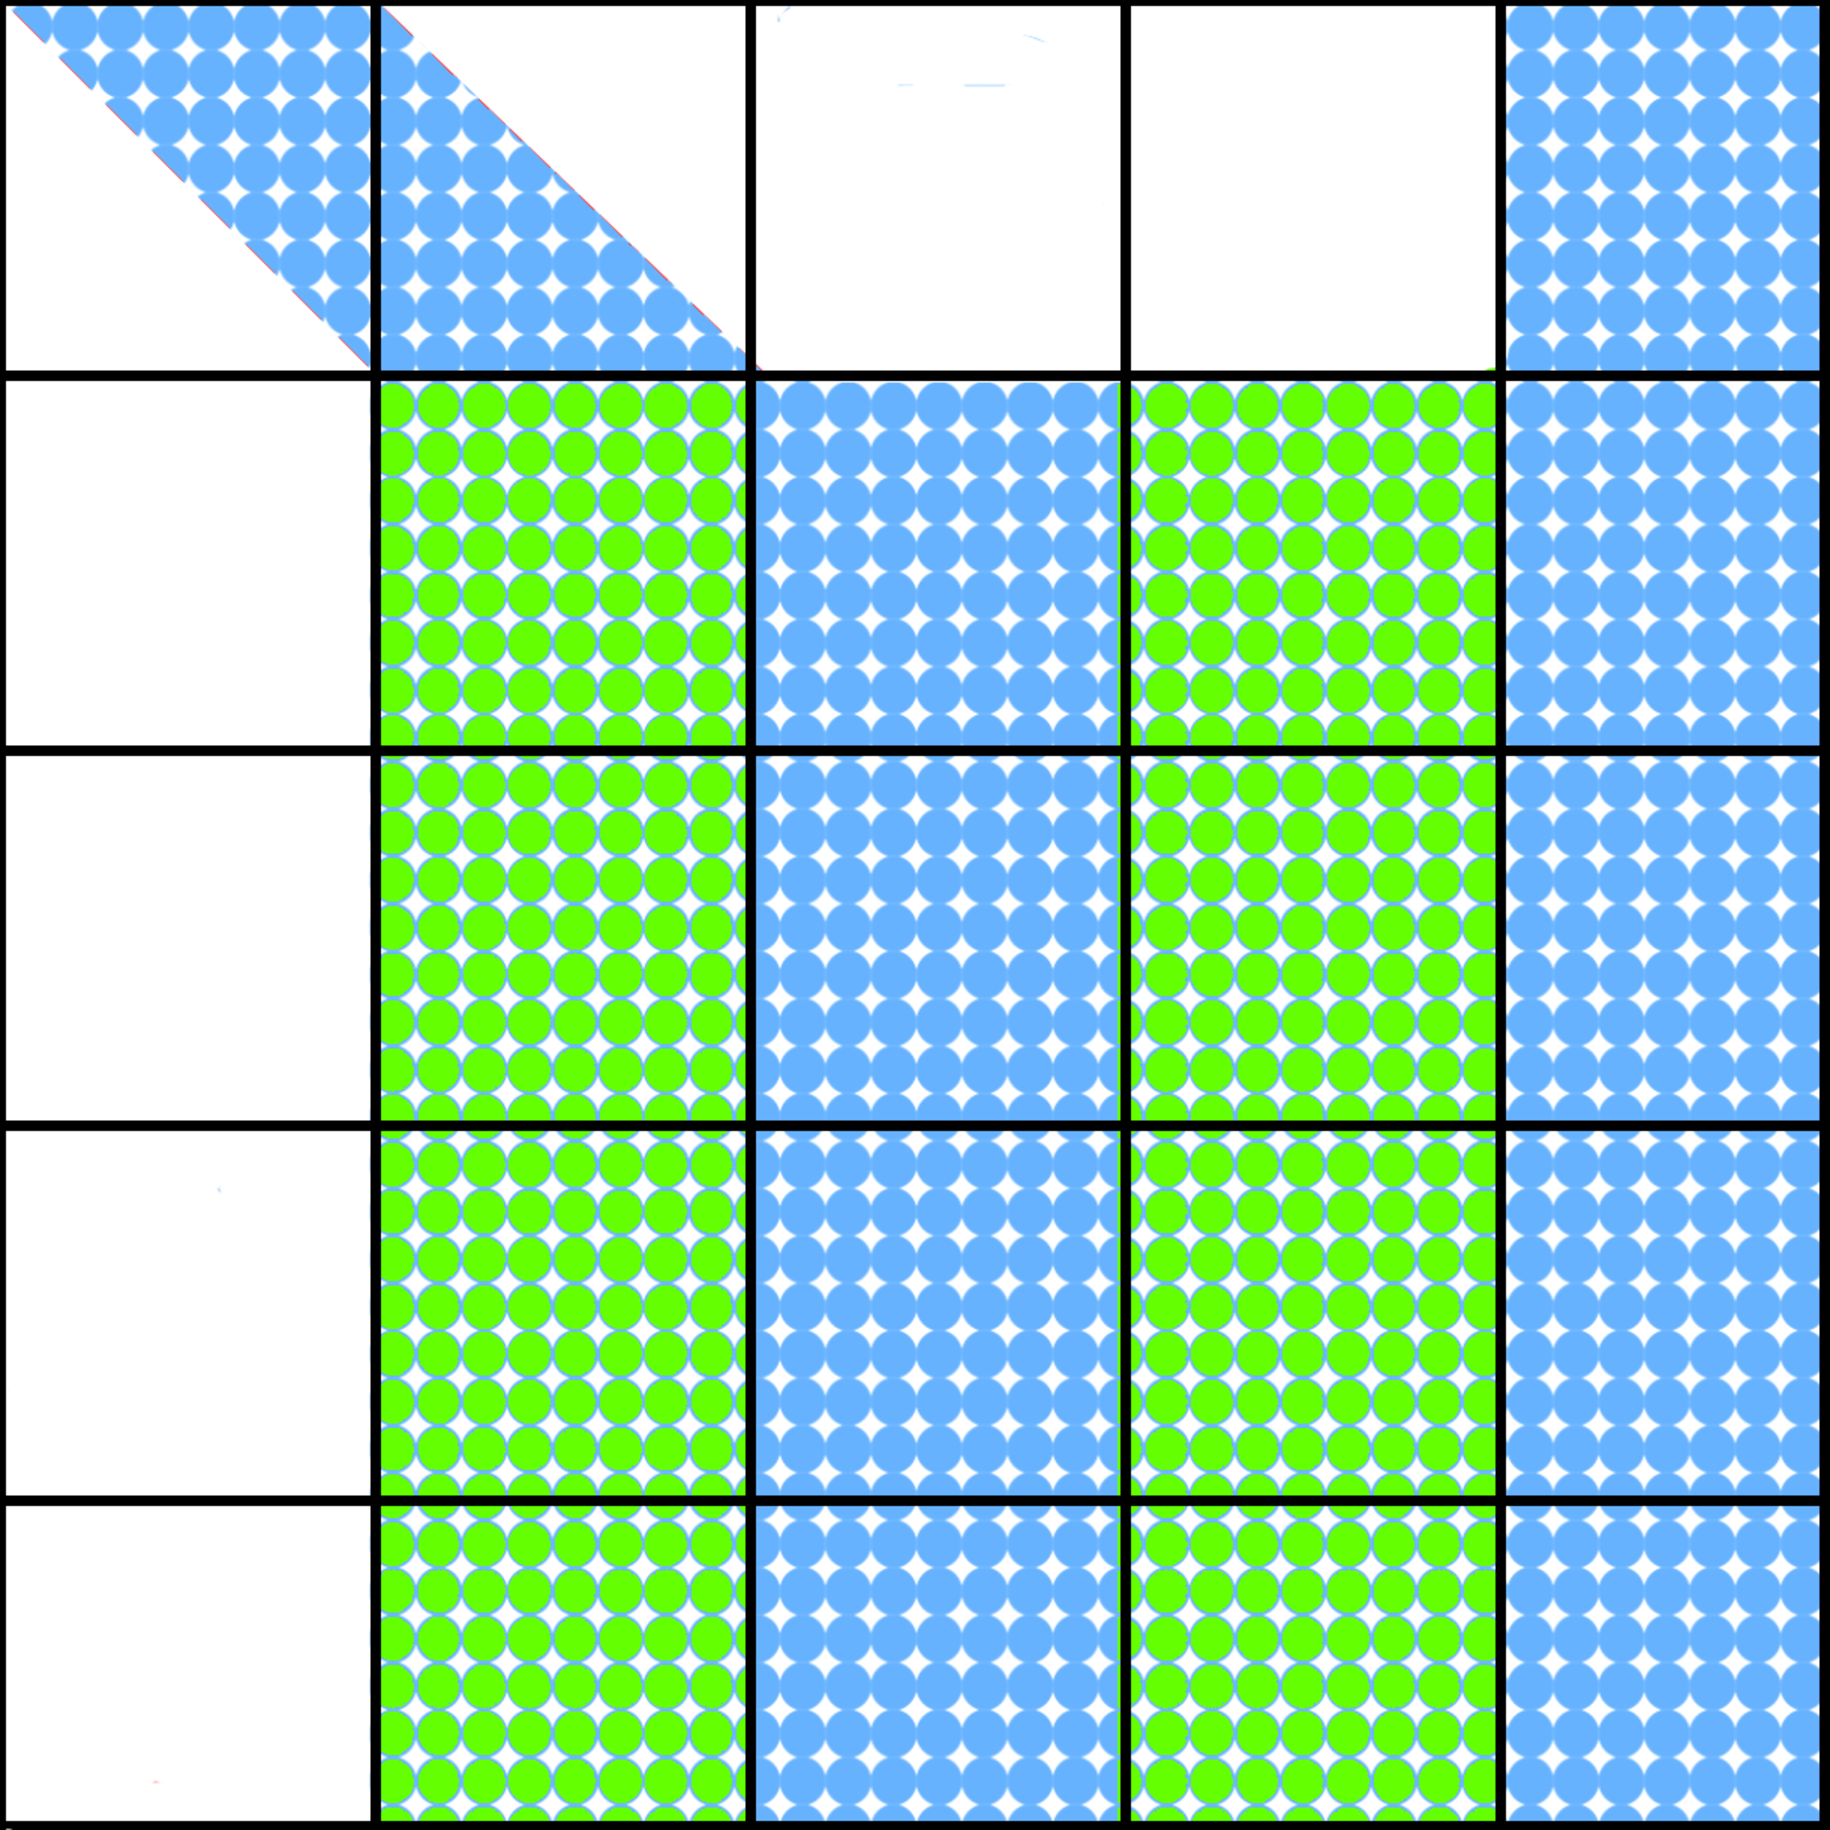
\includegraphics[width=\textwidth]{fig/SVD_tile_12_grid}
    \caption{\label{fig:tile_lq_update_2}Panel update}
  \end{subfigure}
  \hfill

  \caption{Reduction from general matrix to band bidiagonal form
    using early update strategy.
    \label{fig:tile}}
\end{figure}

As illustrated in the DAG (Figure~\ref{fig:dag_tile}),
the early update approach considerably reduces the severity of the
synchronization points.
However,
all the ZUNMQR kernels in charge of updating the
first tile-row have to be completed before starting
any TSQRT kernel,
since the ZUNMQR kernels use the entries of the top left tile and
those entries will be overwritten if any TSQRT kernels are
launched before the end of the first tile-row update.
This explains the bottleneck at TSQRT(2,1) in the DAG.
But the completion of the first TSQRT kernel unlocks many tasks
and leads to high levels of parallelism.


\begin{figure}[h!]
  \begin{center}
    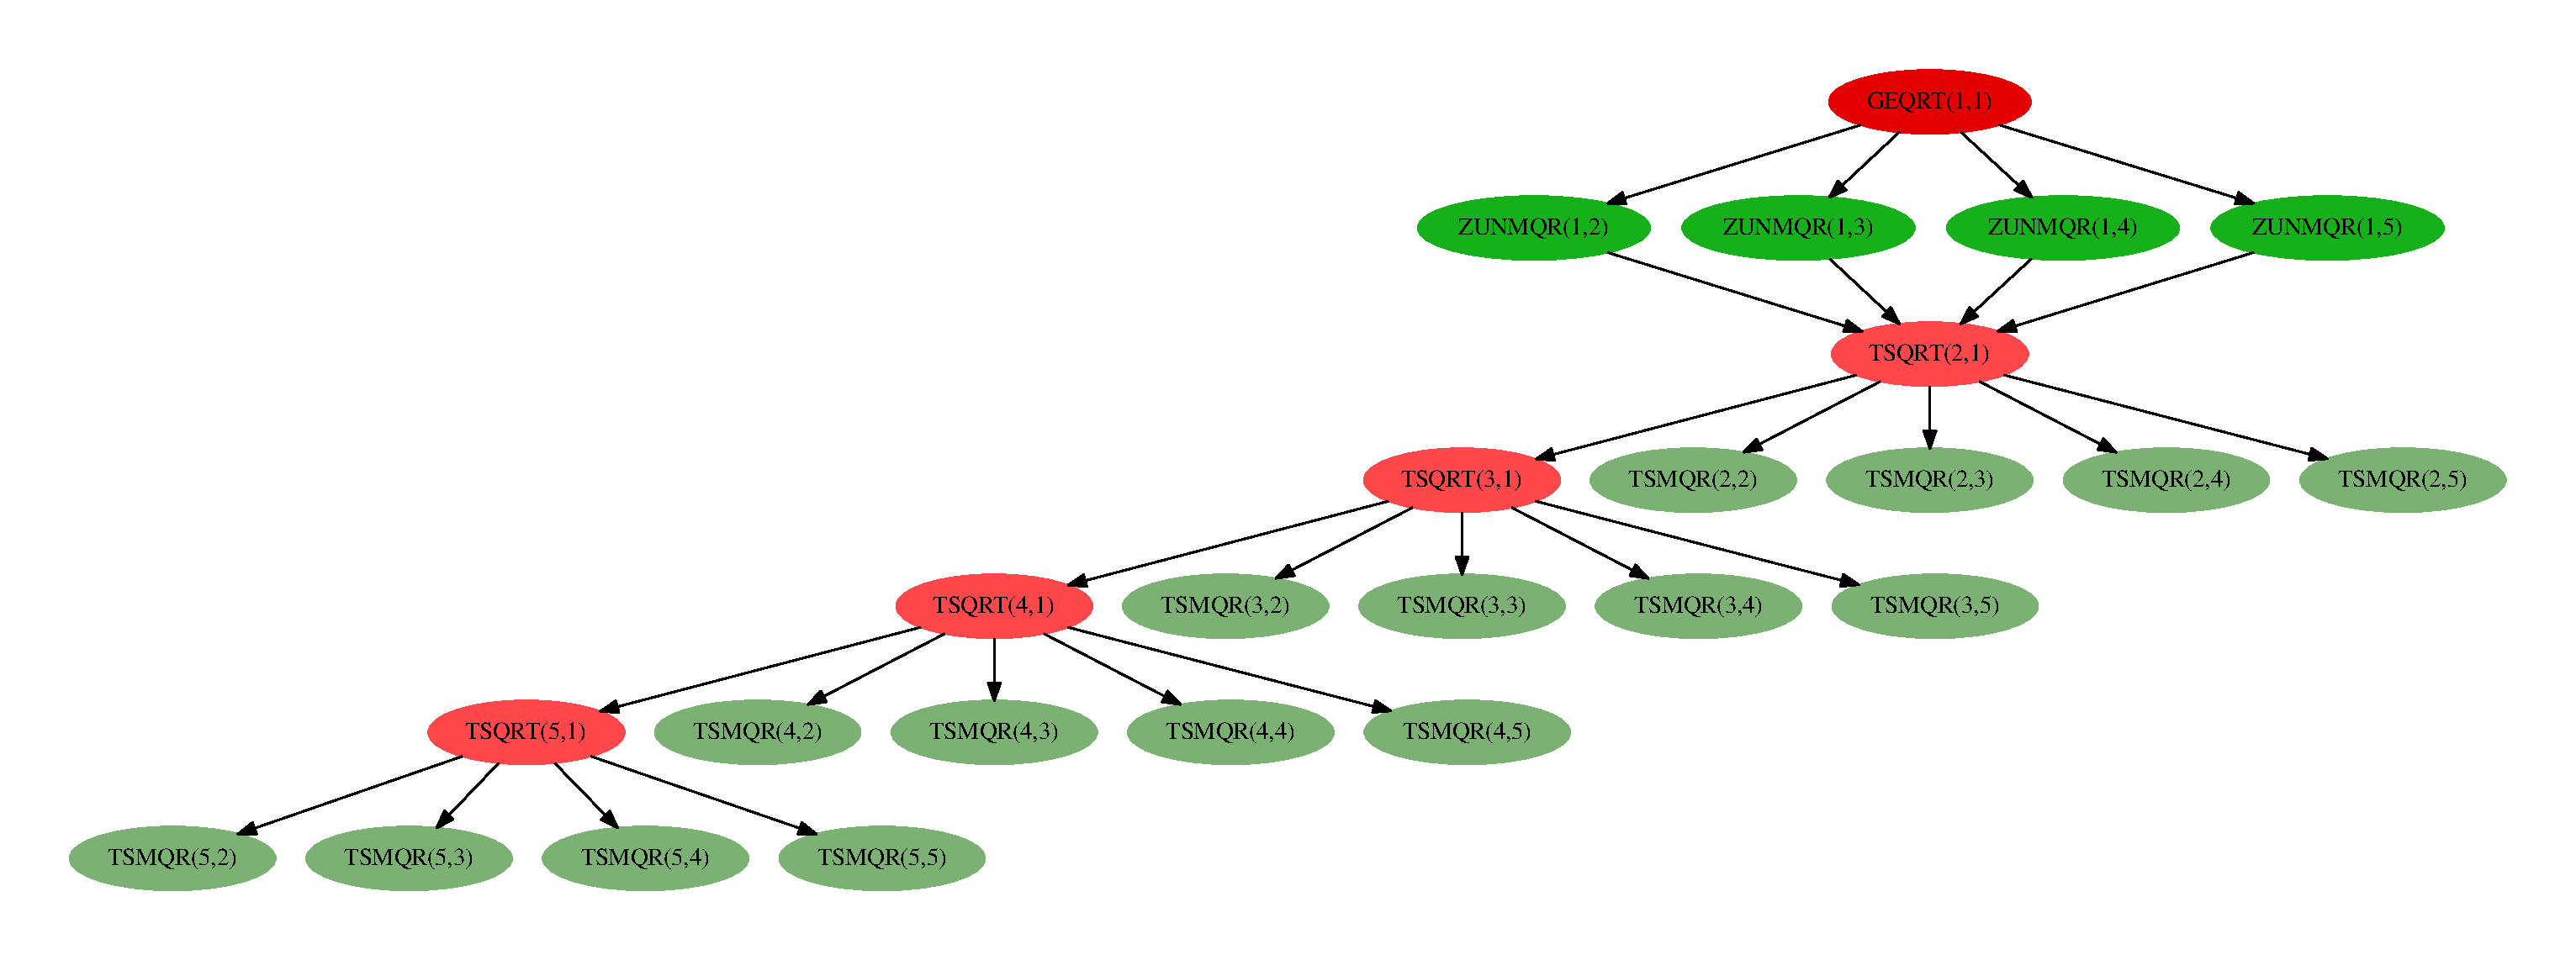
\includegraphics[width=1\textwidth]{fig/dag_tile}
  \end{center}
  \caption{DAG for the early update strategy for band reduction:
    this partial view is limited to the factorization of the first panel and
    the update of the corresponding trailing matrix.}
  \label{fig:dag_tile}
\end{figure}

\subsection{Experimental results}
In order to assess the performance of each strategy,
we design an OpenMP task-based version of each of the two strategies.
In all the experiments within this section,
\texttt{Early update} and \texttt{Late update} will denote
the two strategies explained above, respectively.
We also compare these strategies to the PLASMA 2.8.0 kernel
designed for reduction of a full matrix to band bidiagonal form.
The experiments have been performed with a
NUMA node (two-socket Xeon(R) CPU E5-2650 v3 @ 2.30GHz--Haswell)
and a 68-core
Intel KNL\footnote{https://ark.intel.com/products/94035/Intel-Xeon-Phi-Processor-7250-16GB-1\_40-GHz-68-core}
and all the computations are done in double precision arithmetic.
The performance (GFlop/s) displayed is calculated by dividing the
standard theoretical flops by the time to solution.

\begin{figure}[h!]
  \begin{subfigure}[t]{0.5 \textwidth}
    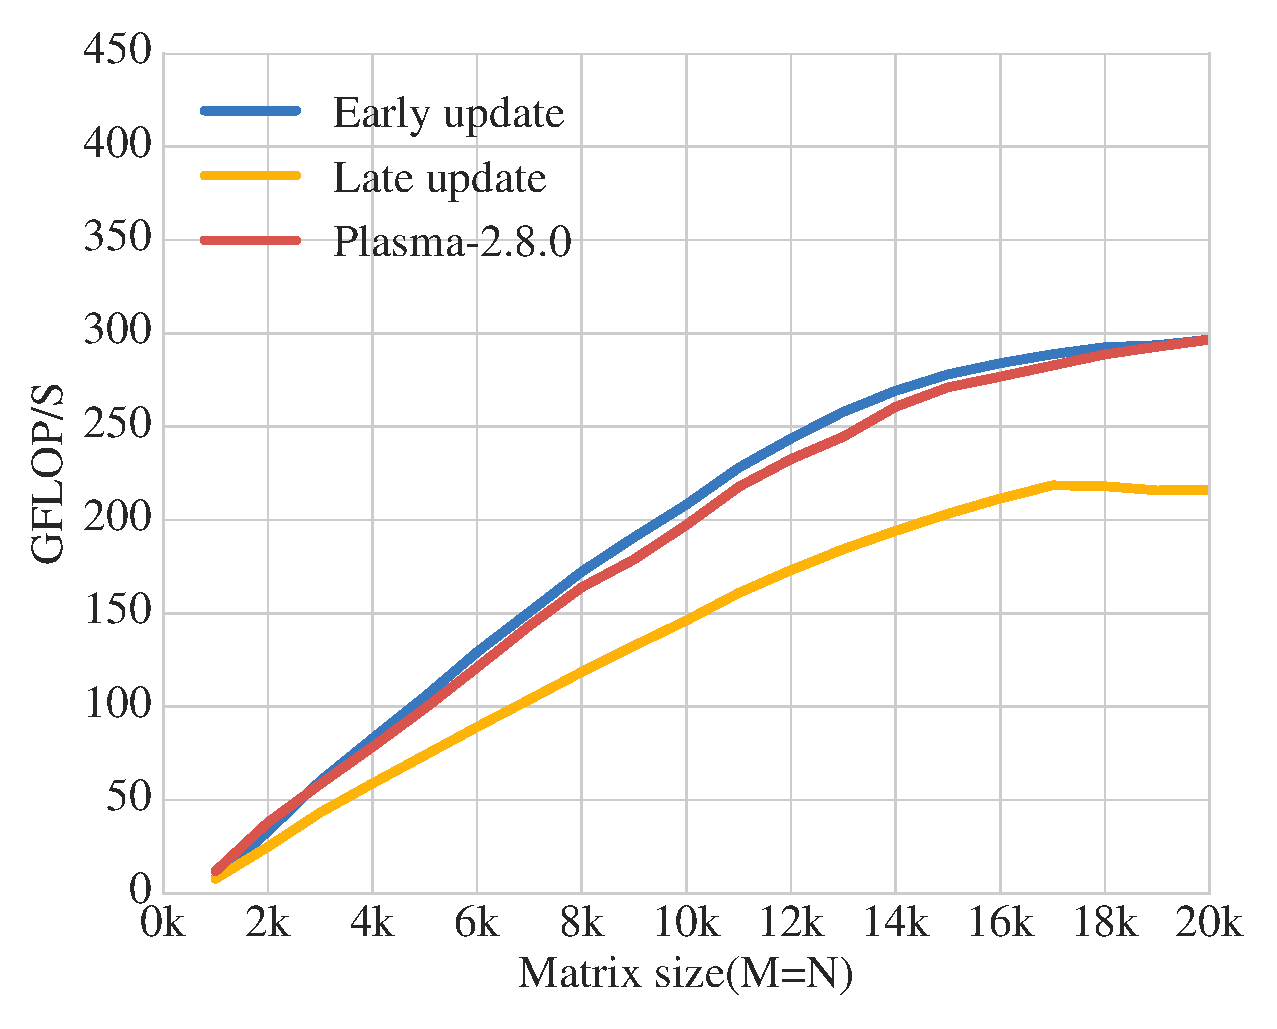
\includegraphics[width=\textwidth]{fig/dge2gb_KNL}
    \caption{\label{fig:dge2gb_DDR4}
      Results with DDR4}
  \end{subfigure}
  \hfill
  \begin{subfigure}[t]{0.5 \textwidth}
    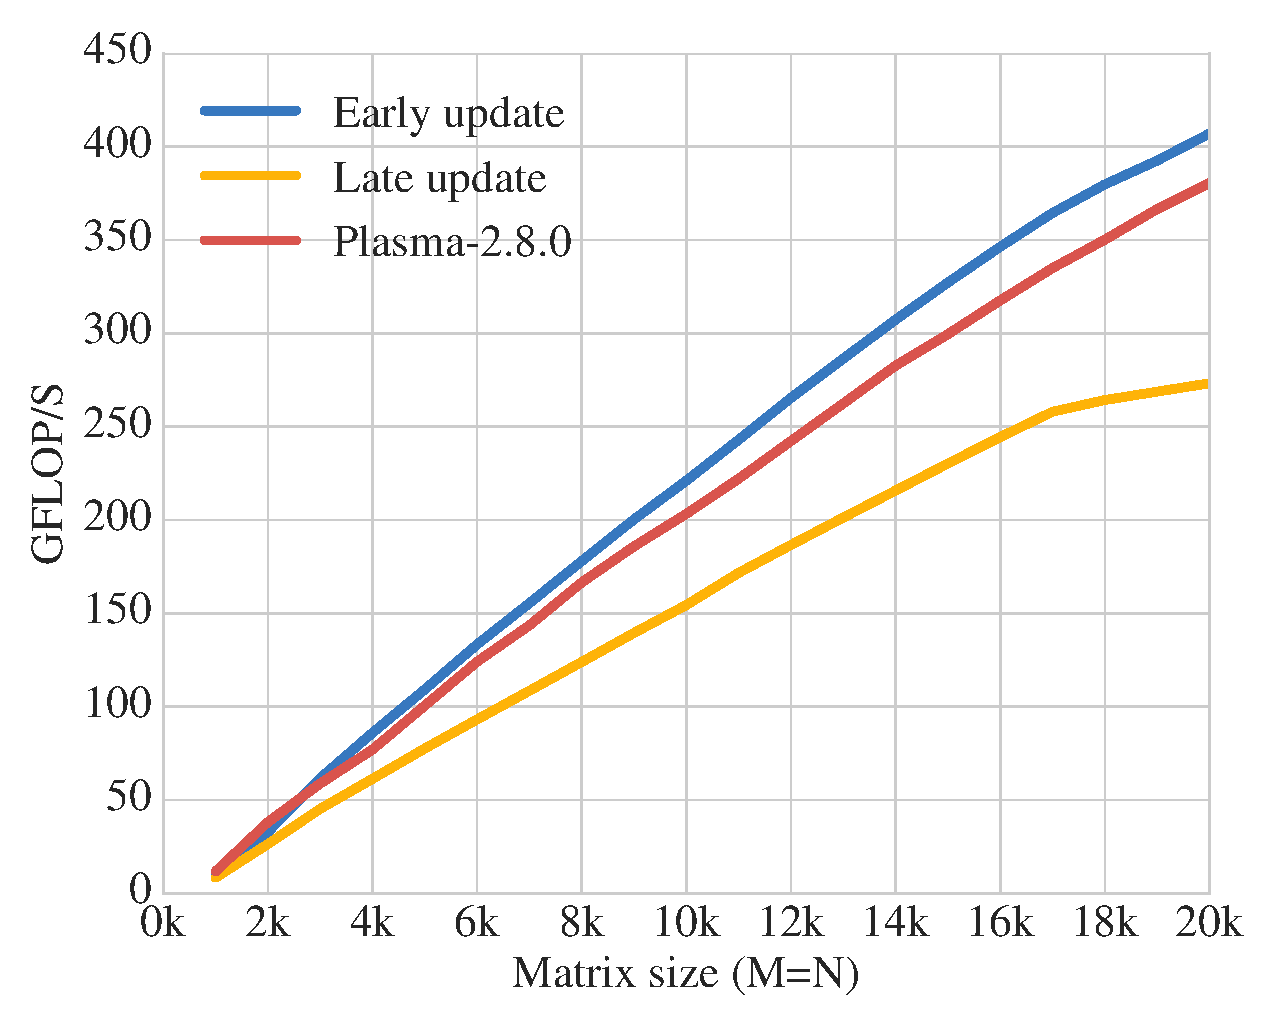
\includegraphics[width=\textwidth]{fig/dge2gb_KNL_HBW}
    \caption{\label{fig:dge2gb_HBW}
      Results with MCDRAM}
  \end{subfigure}
  \caption{Performance comparison of different implementations of
    DGE2GB using $68$ threads on the Intel KNL with square matrices
    ranging in size from $1,000 \times 1,000$ to $20,000 \times
    20,000$.}
  \label{fig:dge2gb_KNL}
\end{figure}


\begin{figure}[h!]
  \begin{subfigure}[t]{0.5 \textwidth}
    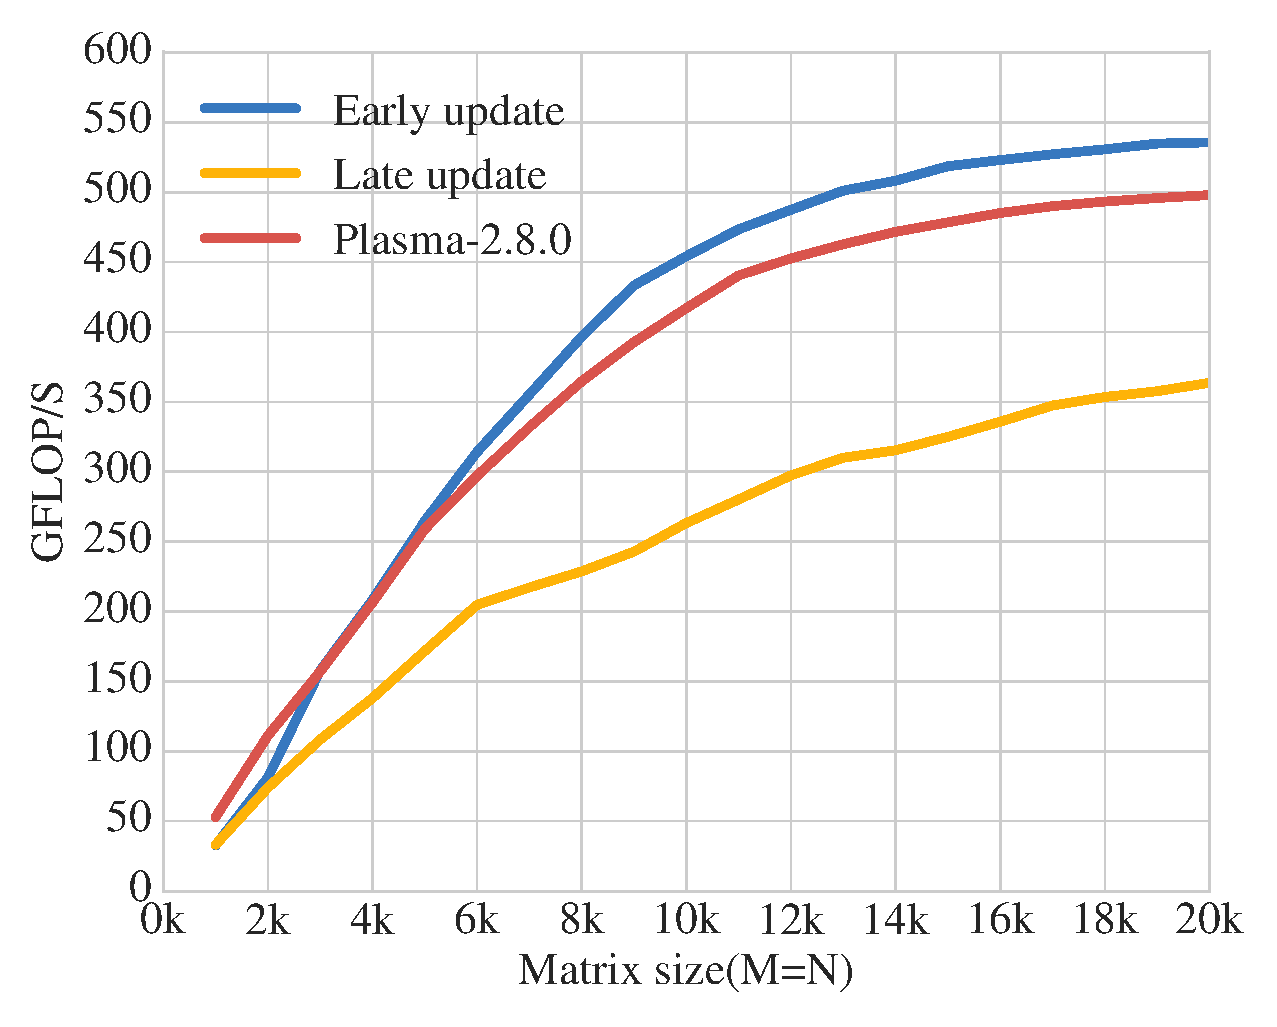
\includegraphics[width=\textwidth]{fig/dge2gb_HASWELL}
    \caption{\label{fig:dge2gb_HASWELL_20}
      Results with 20 threads}
  \end{subfigure}
  \hfill
  \begin{subfigure}[t]{0.5 \textwidth}
    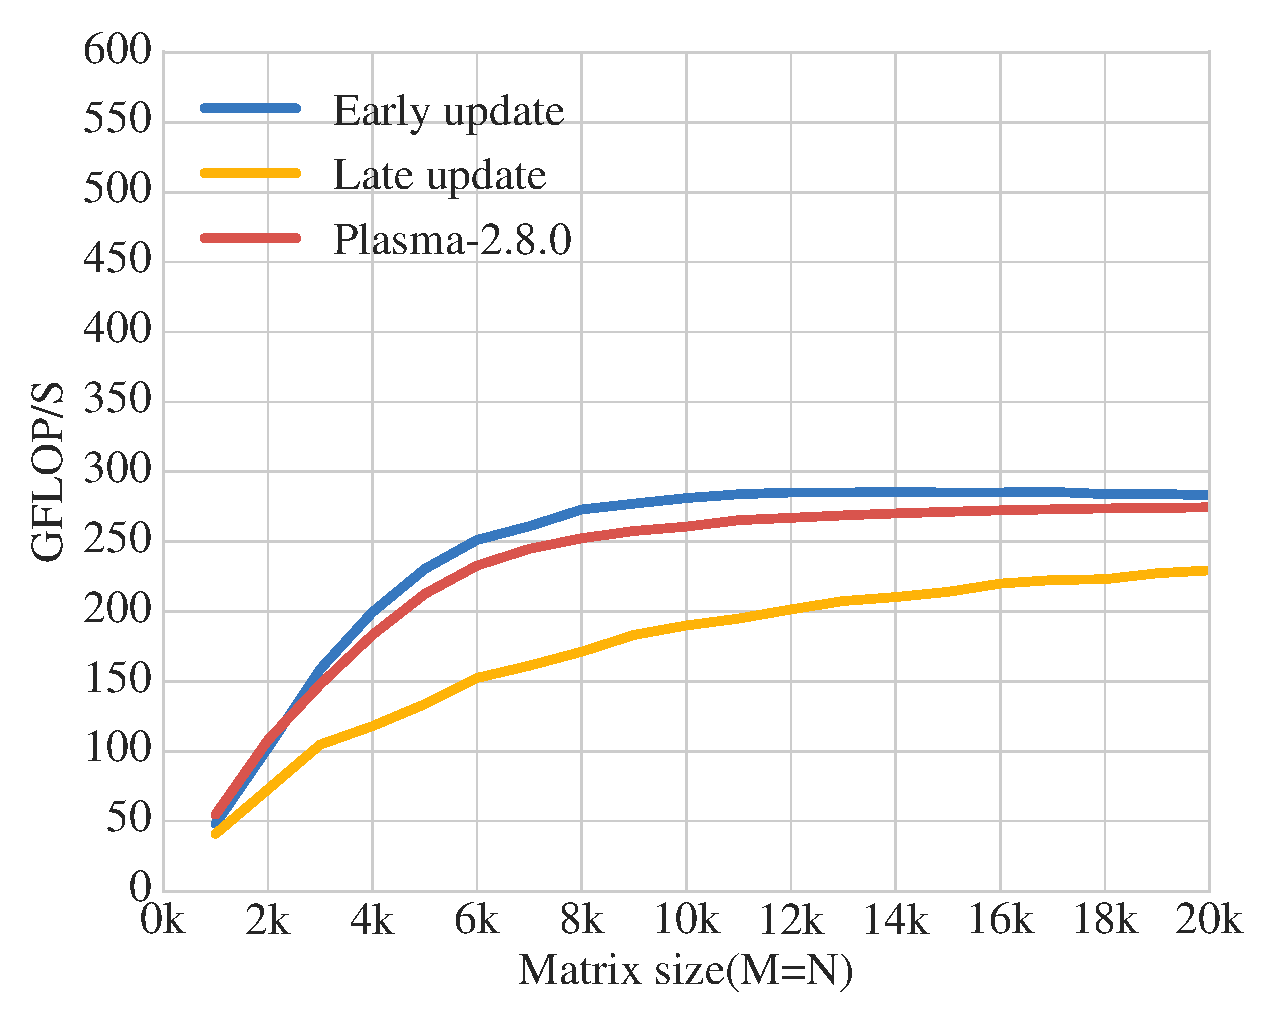
\includegraphics[width=\textwidth]{fig/dge2gb_HASWELL_10}
    \caption{\label{fig:dge2gb_HASWELL_10}
      Results with 10 threads}
  \end{subfigure}
  \caption{Performance comparison of different implementations of
    DGE2GB on a 2x Intel Xeon(R) CPU E5-2650 v3 @ 2.30GHz (20 cores),
    with square matrices ranging in size from $1,000 \times 1,000$ to
    $20,000 \times 20,000$. The experiment with 20 threads is performed
    with the NUMA configuration "numactl --interleave=all" while the
    experiment with 10 threads using only one 10-core socket.}
  \label{fig:dge2gb_HASWELL}
\end{figure}

In addition to the traditional DDR4, the Intel KNL has a high
bandwidth memory called Multi-Channel DRAM (MCDRAM) with a
bandwidth four times greater than the DDR4 bandwidth,
but with a storage capacity limited to 16GB.
There are different configuration options
of MCDRAM, but in this experiment it has been configured
in flat mode i\@.e\@.~the 16GB memory can be directly allocated from within
an application as is the case for DDR4.
In our experiments we provide results for both DDR4 and MCDRAM.

As illustrated in Figure~\ref{fig:dge2gb_DDR4} where the data is
allocated in DDR4, the early update approach gives the best
performance with a slight advantage over the Plasma-2.8.0
implementation.
The significant gap between the early update and late update
strategies is consistent with our expectations
and confirms the benefit of the early update strategy.
In Figure~\ref{fig:dge2gb_HBW} where data is allocated in
the MCDRAM instead of the regular DDR4, the difference between the
strategies is fairly similar,
although all implementations benefit from the increased memory access
speed.

We obtained a similar result on a NUMA node (2x Intel Xeon(R)
CPU E5-2650 v3) using 20 threads and 10 threads in
Figure~\ref{fig:dge2gb_HASWELL_20} and
Figure~\ref{fig:dge2gb_HASWELL_20} respectively.
However, unlike for the 68-core Intel KNL,
the late update strategy exhibits a more severe
performance penalty.

In the next subsection we investigate ways to remove
the bottlenecks in both synchronisation points in both
the early and late update strategies.

\subsection{Potential improvements}
One way to solve the performance issue discussed for both the
late update and the early update strategy is to revisit the
data dependencies and remove all unnecessary synchronizations.
In Figure~\ref{fig:panel} for example,
since the algorithm is task based,
a part of the trailing matrix update in Figure~\ref{fig:qr_update_1}
could start before the completion of the panel factorization
(Figure~\ref{fig:qr_1}), if its dependencies are satisfied.
In the same way,
once the first tile-row is updated,
the update of the other tile-rows below could follow as
soon as their corresponding tile in the panel is eliminated.
Unfortunately, all these parallelisms are not exploited
in the version presented above.

In fact, the update of the first tile-row uses the top
left corner tile $A(1,1)$ as input (read dependency), while the TSQRT
kernel in charge of the elimination of the square tiles in the panel
modifies $A(1,1)$ (read and write dependency). The update kernel then
waits until the completion of the panel factorization. But a further
analysis of the algorithm helps to realize that as illustrated in
Figure~\ref{fig:rect_panel}, that once $A(1,1)$ is factorized the
elimination operations applied to the rest of the panel modify only
the upper triangular part of $A(1,1)$. On the other hand, the update
of the first tile-row requires only reflectors stored in the lower
triangular part of $A(1,1)$.
Therefore the panel factorization and the update of
the first tile-row could be done in parallel.

Currently our OpenMP implementation supports dependencies only
between full tiles.
This introduces an unnecessary dependency between
the first tile-row update and the first tile-column
elimination through the $A(1,1)$ tile.
To solve this we might want to
split all $A(i,i)$ tiles into upper and lower parts.

Alternatively, one can modify the way OpenMP expresses
its data dependencies.
To illustrate this, lets consider an $nb \times nb$ tile $B$.
The standard way to express a read or input dependency on $B$ is
\begin{lstlisting}
  #pragma omp task depend(in:B[0:nb*nb])
\end{lstlisting}
while write or output dependency on B would be
\begin{lstlisting}
  #pragma omp task depend(out:B[0:nb*nb]).
\end{lstlisting}

The OpenMP runtime system then ensures that the dependency criteria
are satisfied on each of the $nb \times nb$ entries before executing
the corresponding kernel. But instead of using
\texttt{depend(in:B[0:nb*nb])}, if one uses \texttt{depend(in:B[i])},
the runtime system will check only the $i^{th}$ entry of the tile to
decide whether to execute the kernel or not. Although specifying the
whole ranges is the recommended way, using only a single entry is an
alternative in cases where only some entries of the tile are used and
the $i^{th}$ entry is representative of their dependency. Since the
tile entries are stored in column major format, an input and output
dependency on the upper triangular tile can be simulated by
\texttt{\#pragma omp task depend(inout:B[0])} (zero is the starting
index of the upper triangular tile with respect to C language and
column major storing) and an input dependency on the
lower triangular by \texttt{\#pragma omp task depend(in:B[1])} (one is
the starting index of the lower triangular tile).

Expressing tile dependency at upper/lower triangular
granularity helps us achieving a highly parallel kernel as
demonstrated by the corresponding DAG depicted in Figure~\ref{fig:dag_hack}.
\begin{wrapfigure}{r}{0.5\textwidth}
  \begin{center}
    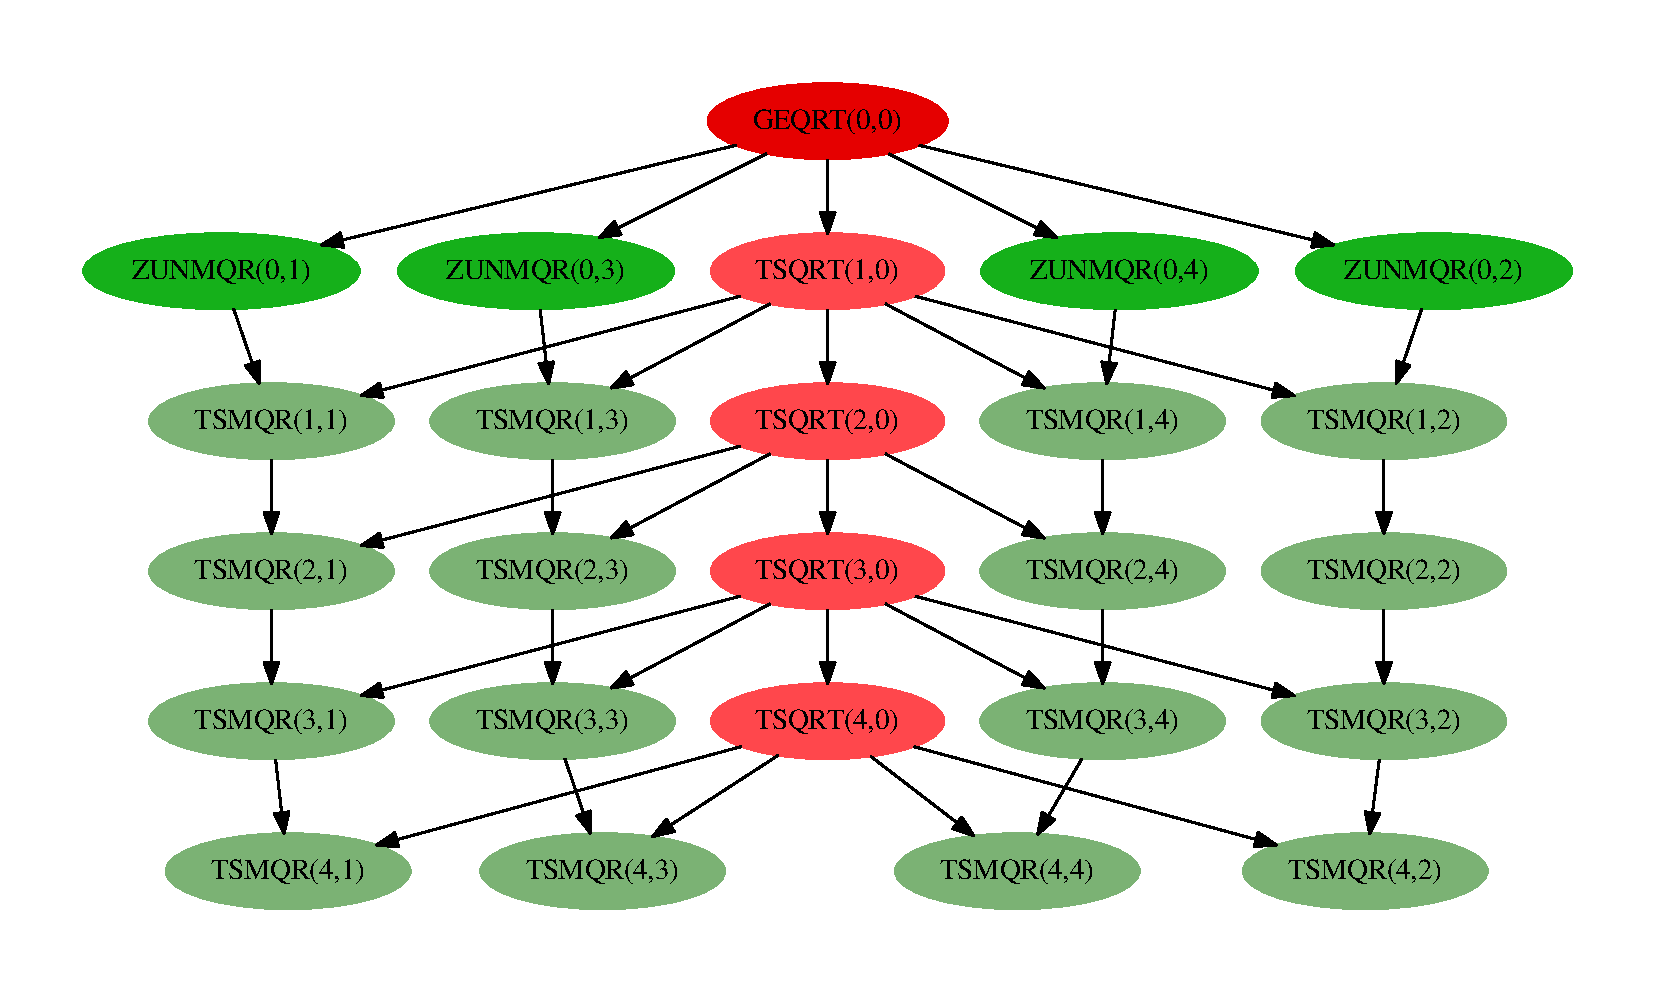
\includegraphics[width=0.48\textwidth]{fig/dag_better}
  \end{center}
  \caption{DAG for the late update strategy for band reduction when
      $A(i,i)$ dependencies are expressed at the upper/lower tile
      granularity. This partial view is limited to the factorization of the
      first panel and the update of the corresponding trailing matrix.}
  \label{fig:dag_hack}
\end{wrapfigure}

We also applied this modification to the early update strategy
to remove the synchronisation point observed previously.
In fact, since we are working at the triangular tile granularity this
releases all unnecessarily dependencies,
the panel and tile strategies should provide comparative results.

To assess the effectiveness of this improvement,
We reproduced the same experiments but now with
some critical dependencies expressed at triangular
tile granularity.

The effectiveness of the modification is illustrated by
the improvement of the Intel 68-core KNL performance
results in Figure~\ref{fig:dge2gb_KNL_HACK} where
the early update and the late update strategies
almost overlap and both are slightly better than Plasma-2.8.0.
This observation is consistent with results with DDR4 as well as
for results with MCDRAM.
There is also a slight improvement in the
performance achieved by the early update strategy
compared to the results in Figure~\ref{fig:dge2gb_KNL} where all dependencies
were expressed at full tile granularity.
We have also observed similar results for the experiments
illustrated in Figure~\ref{fig:dge2gb_HASWELL} with the Intel Haswell NUMA node.


\begin{figure}[h!]
  \begin{subfigure}[t]{0.5 \textwidth}
    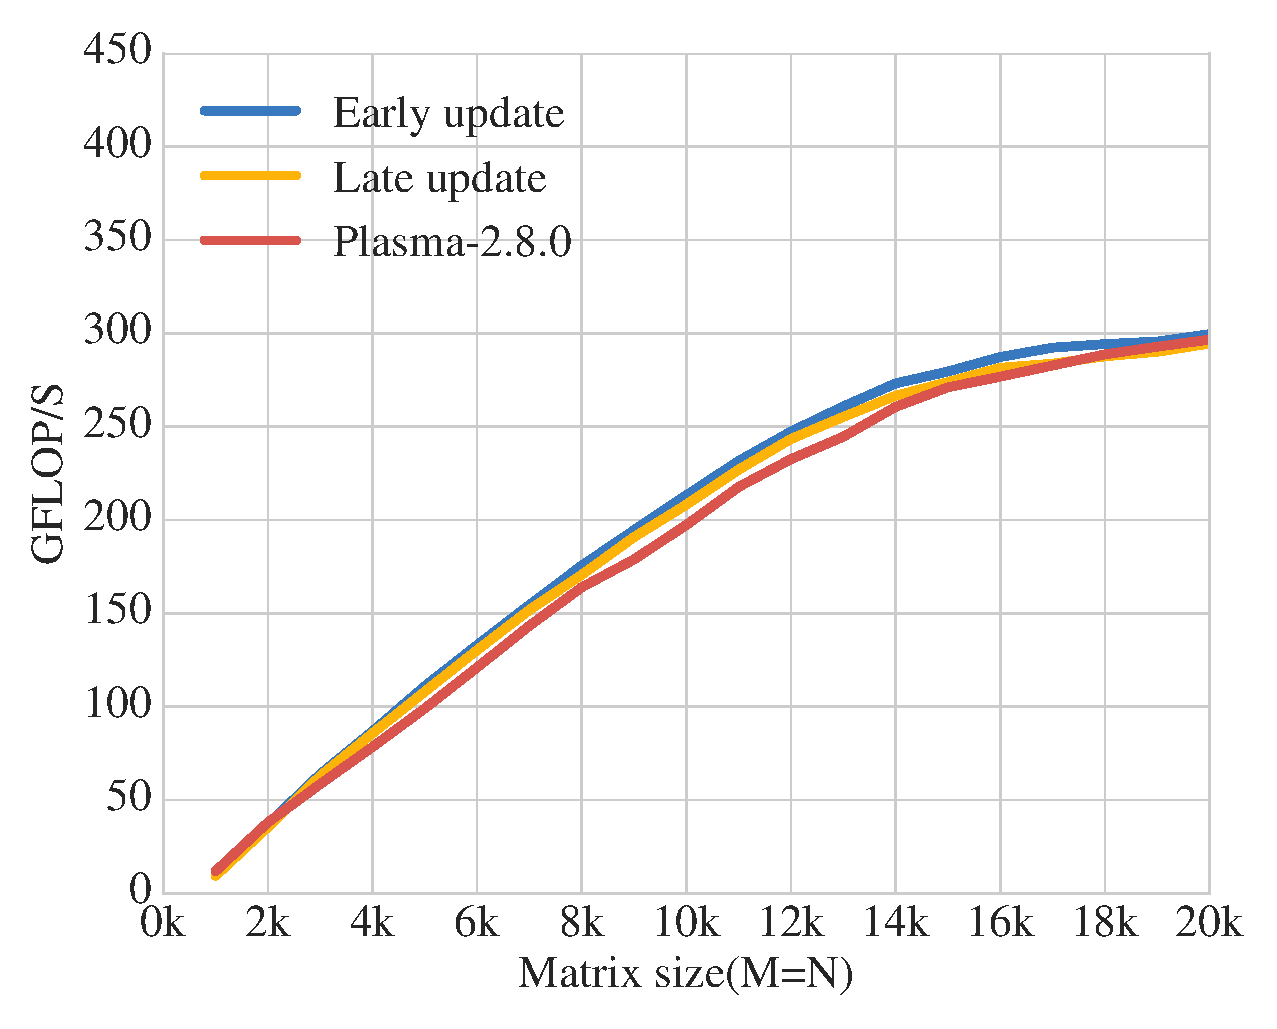
\includegraphics[width=\textwidth]{fig/dge2gb_KNL_HACK}
    \caption{\label{fig:dge2gb_DDR4_HACK}
      Results with DDR4}
  \end{subfigure}
  \begin{subfigure}[t]{0.5 \textwidth}
    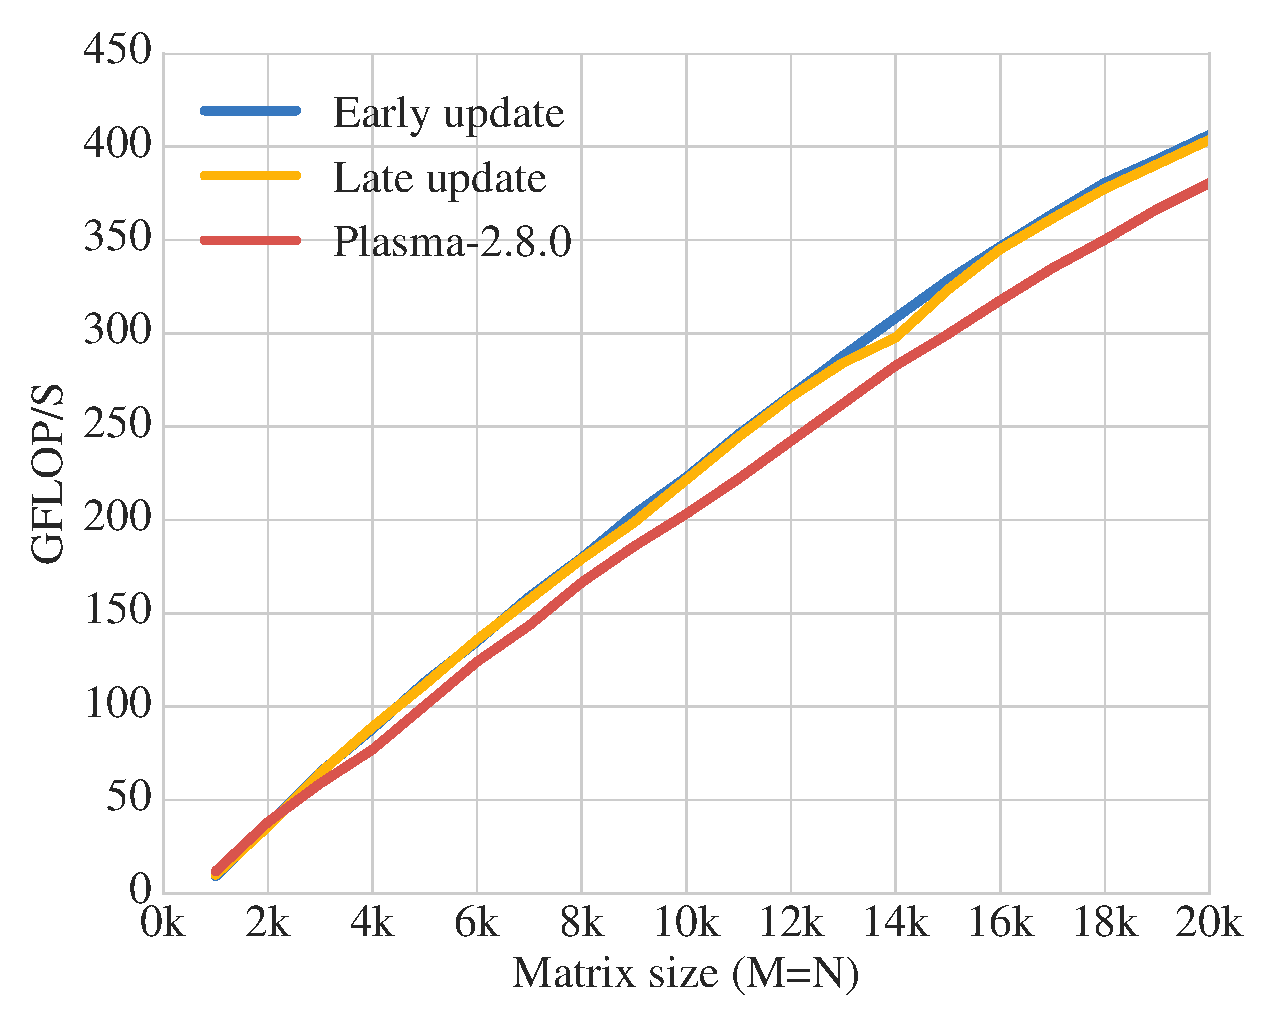
\includegraphics[width=\textwidth]{fig/dge2gb_KNL_HACK_HBW}
    \caption{\label{fig:dge2gb_HBW_HACK}
      Results with MCDRAM}
  \end{subfigure}
  \caption{Performance comparison of different implementations of
    DGE2GB using $68$ threads on the Intel KNL with different
    square matrices ranging in size from $1,000 \times 1,000$ to $20,000 \times 20,000$.
    The code has been modified to  express some
    data dependencies at \texttt{upper/lower triangular tile} granularity.}
  \label{fig:dge2gb_KNL_HACK}
\end{figure}


\begin{figure}[h!]
  \begin{subfigure}[t]{0.5 \textwidth}
    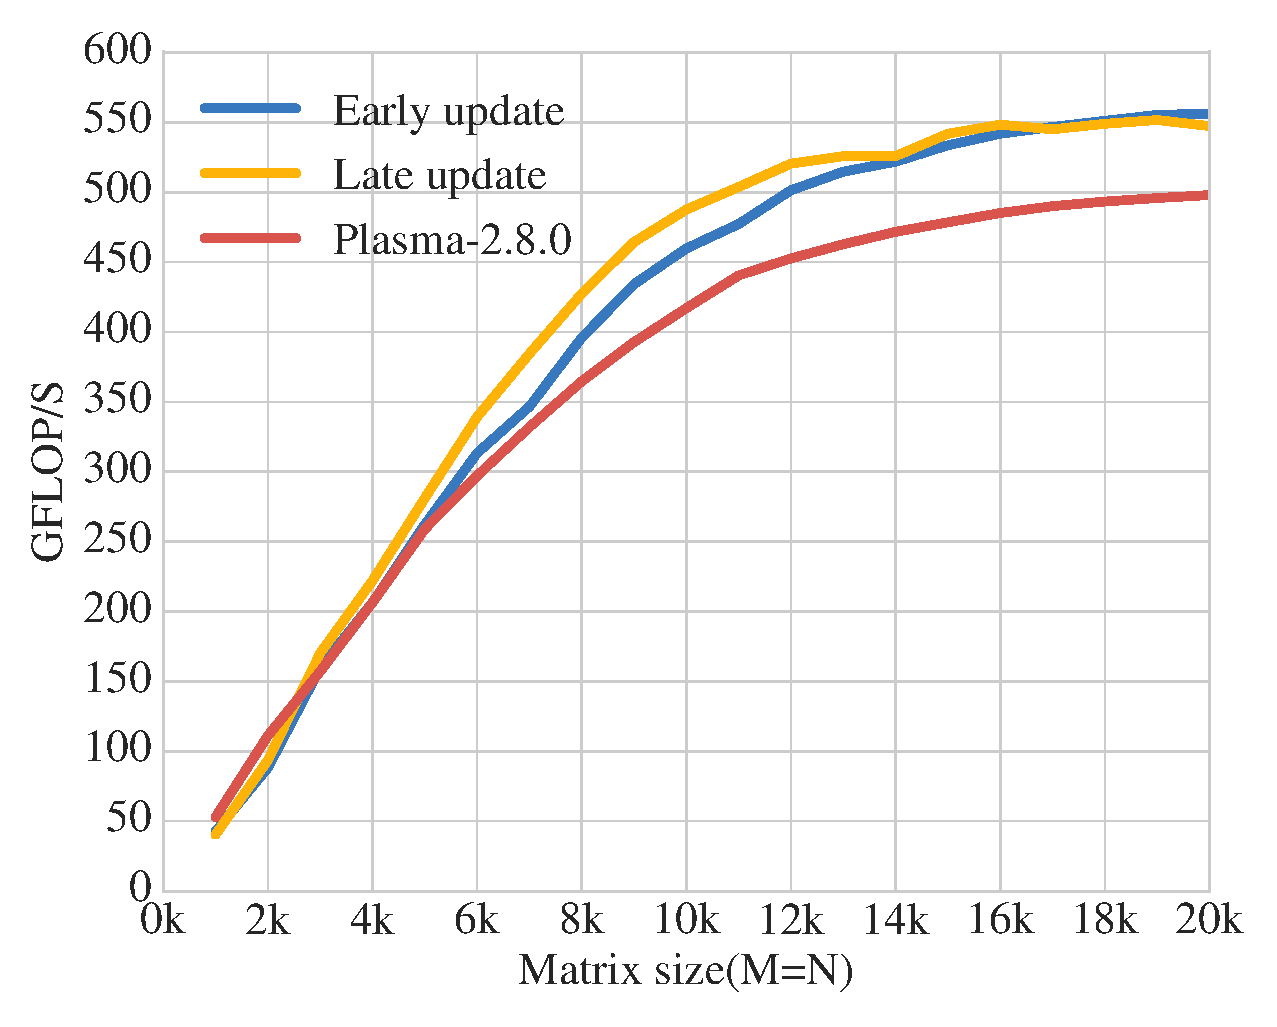
\includegraphics[width=\textwidth]{fig/dge2gb_HASWELL_HACK}
    \caption{\label{fig:dge2gb_HASWELL_20}
      Results with 20 threads}
  \end{subfigure}
  \hfill
  \begin{subfigure}[t]{0.5 \textwidth}
    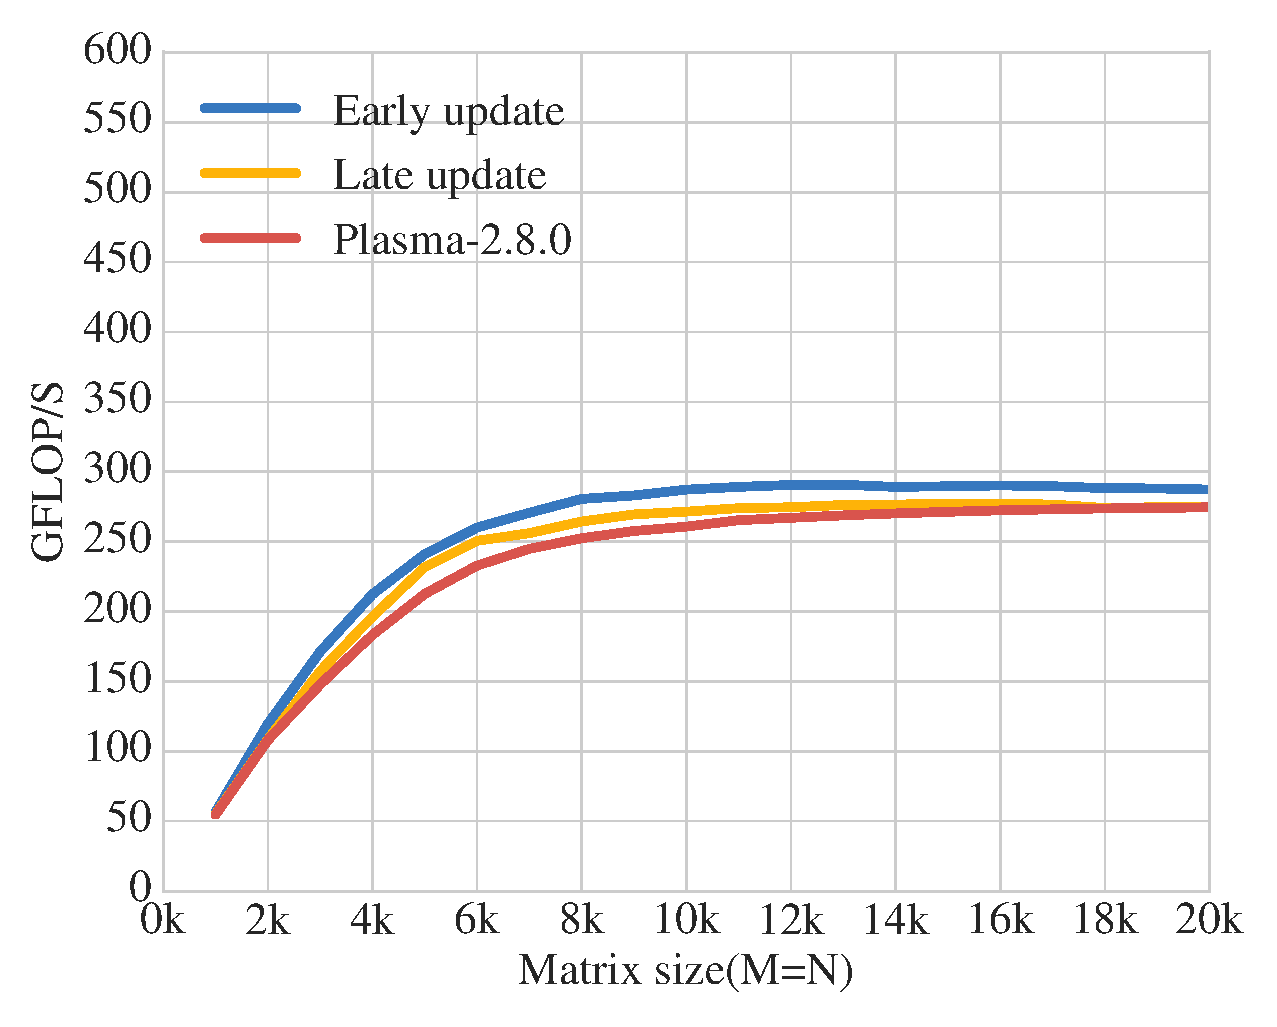
\includegraphics[width=\textwidth]{fig/dge2gb_HASWELL_HACK_10}
    \caption{\label{fig:dge2gb_HASWELL_10}
      Results with 10 threads}
  \end{subfigure}
  \caption{Performance comparison of different implementations of
    DGE2GB on a NUMA node with
    2x Intel Xeon(R) CPU E5-2650 v3 @ 2.30GHz (20 cores),
    with square matrices ranging in size from $1,000 \times 1,000$ to
    $20,000 \times 20,000$. The experiment with 20 threads is performed
    with the NUMA configuration "numactl --interleave=all" while the
    experiment with 10 threads used only one 10-core socket.
    The code has been modified to  express some
    data dependencies at \texttt{upper/lower triangular tile} granularity.}
  \label{fig:dge2gb_HASWELL}
\end{figure}

As reported in~\cite{haidar2013improved},
the SVD implementation based on the
Plasma-2.8.0 bidiagonalization kernel could be two times faster than
Intel’s Math Kernel Library (MKL), when all the singular vectors are
requested and up to 10 times faster if only the singular values are
required. This shows the efficiency of the Plasma-2.8.0 bidiagonalization
kernel, and the performance of our OpenMP implementation
in comparison with Plasma-2.8.0 demonstrates the effectiveness of our prototype.

Furthermore, working at triangular tile granularity only gains
a slight performance improvement for the early update
strategy,
whilst it requires declaring OpenMP dependencies in a
non-conventional way.
For this reason, it makes sense to keep the tile
oriented strategy with dependencies at full tile granularity,
as it is reasonably efficient and respects the standard OpenMP programming
conventions.
In addition by declaring data dependencies in a conventional
way, the code can be safely extended to a distributed memory environment.
